%%% thesis.tex
%%% no more needs to be said
%
% Alex Barnett, Sept 2000.
%
% Taken from Adam Lupu-Sax and edited May 2000.

% my preferred settings:
% \documentclass[11pt,twoside,final]{huthesis}

% Harvard GSAS Jan 2000 settings:
% (Lauren Lamir 5-1519 gave 12pt Times New Roman as the ideal size)...
\documentclass[12pt,oneside,final]{huthesis}


\usepackage{epsfig,bm,epsf,float}
\usepackage{graphicx}
\usepackage{amsfonts}
\usepackage{amsmath}
\usepackage{amssymb}
\usepackage{dsfont}
\usepackage[usenames]{color}
 
\usepackage{dcolumn}% Align table columns on decimal point
\usepackage{bm}% bold math
\usepackage{color}
\usepackage{hyperref}% add hypertext capabilities
 
%% choose which files to process
%% stolen from the mitthesis suite
% \typein [\files]{Enter file names to process, (frontmatter,intro,
%   ...), or `all' to process all files:}
% \def\all{all}
% \ifx\files\all
% \typeout{Including all files.} \else \typeout{Including only \files.}
% \includeonly{\files}
% \fi

% Table of contents max depth listed:
% 1 = section, 2 = subsection, 3 = subsubsection
% (Adam Lupu-Sax had 1. Is this standard at Harvard? I'm going for 2)
\setcounter{tocdepth}{2}


\begin{document}

\input{mathdefs} % my math definitions.


% UNDERLYING SPACING FOR WHOLE DOCUMENT:
% Single spacing: takes place of `draft' mode, without losing figures.
% \ssp

% makes double-spaced: (for GSAS requirement, microfiche):
\dsp 


%% frontmatter.tex
%%

\title{Systems and Protocols for Quantum Metrology and Quantum Computation}
\author{P\'{e}ter K\'{o}m\'{a}r}
\degreemonth{December} % month final submission occurs.
\degreeyear{2015}
\degree{Doctor of Philosophy}
\field{Physics} 
\department{Physics}
\advisor{Mikhail D. Lukin} % Category I added.

\maketitle
\copyrightpage
  

\begin{abstract} 
% limited to 1.5 pages, double-spaced (Registrar's Office guidelines).
% Also limited to 350 words. I claim $\mu \sim \omega^4$ is a single word.
   
Abstract about 
\begin{itemize}
  \item Quantum computation protocols
  \item and their use
  \item Quantum metrology protocols
  \item and their use
  \item systems capable of realizing them
  \item namely: optomechanical systems
  \item atomic sytems
\end{itemize} 

\end{abstract}



\newpage
\addcontentsline{toc}{section}{Table of Contents}
\tableofcontents

% these are optional in the Jan 2000 Harvard thesis GSAS guide:
\listoffigures
% use \caption[lst-entry]{Text of table caption} to define the title of the
% figure
\listoftables


% cccccccccccccccccccccccccccccccccccccccccccccccccccccccccccccccccccccccccc
\begin{citations}

\vspace{0.8in}

\ssp
\noindent
Most of the chapters of this thesis have appeared in print elsewhere. By
chapter number, they are:
\begin{itemize}
  	\item 
		Chapter \ref{ch:Komar2013}: 
		``Single-photon nonlinearities in two-mode optomechanics,'' 
		P. K\'{o}m\'{a}r,
		S. D. Bennett, 
		K. Stannigel,  
		S. J. M. Habraken,  
		P. Rabl,  
		P. Zoller, 
		and 
		M. D. Lukin, 
		\emph{Phys.	Rev.  A} 
		\textbf{87}, 
		013839 
		(2013).
  	\item 
		Chapter \ref{ch:Stannigel2012}: 
		``Optomechanical quantum information processing,'' 
		K. Stannigel,  
		P. K\'{o}m\'{a}r, 
		S. J. M. Habraken,  
		S. D. Bennett,
		M. D. Lukin,
		P. Zoller,   
		and P. Rabl, 
		\emph{Phys. Rev. Lett.} 
		\textbf{109},
		013603 (2012).
  	\item 
		Chapter \ref{ch:Borregaard_PRL2015}: 
		``Heralded Quantum Gates with Integrated Error Detection,'' 
		J. Borregaard, 
		P. K\'{o}m\'{a}r, 
		E. M. Kessler, 
		A. S. S{\o}rensen, 
		and M. D. Lukin,
 		\emph{Phys. Rev. Lett.} 
		\textbf{114},
		110502 (2015).
  	\item 
		Chapter \ref{ch:Borregaard_PRA2015}: 
		``Remote entanglement distribution using individual atoms in
  		cavities,'' 
		J. Borregaard, 
		P. K\'{o}m\'{a}r, 
		E. M. Kessler, 
		A. S. S{\o}rensen, 
		and M. D. Lukin, 
 		\emph{Phys. Rev. A} 
		\textbf{92},
		012307 (2015).
  	\item 
		Chapter \ref{ch:Kessler2014}: 
		``Heisenberg-Limited Atom Clocks Based on Entangled Qubits,''
		E. M. Kessler, 
		P. K\'{o}m\'{a}r,  
		M. Bishof, 
		L. Jiang, 
		A. S. S{\o}rensen, 
		J. Ye, 
		and M. D. Lukin,
 		\emph{Phys. Rev. Lett.} 
		\textbf{112},
		190403 (2014).
  	\item 
		Chapter \ref{ch:Komar2014}: 
		``A quantum network of clocks,''
		P. K\'{o}m\'{a}r,  
		E. M. Kessler, 
		M. Bishof, 
		L. Jiang, 
		A. S. S{\o}rensen, 
		J. Ye, 
		and M. D. Lukin,
 		\emph{Nature Physics} 
		\textbf{10},
		582�587 (2014).
	\item 
		Chapter \ref{ch:Komar2015}: 
		``\warn{?}Quantum network of netural atom clocks,''
		P. K\'{o}m\'{a}r,  
		T. Topcu, 
		E. M. Kessler, 
		A. Derevianko, 
		A. S. S{\o}rensen, 
		and M. D. Lukin,
 		\emph{\warn{??}} 
		\textbf{\warn{??}},
		\warn{??} (2015\warn{?}).			 
\end{itemize}

\end{citations}




\begin{acknowledgments}




\end{acknowledgments}





%ddddddddddddddddddddddddddddddddddddddddddddddddddddddddddddddddddddddddddd
\dedication

\begin{quote}
\hsp
\em
\raggedleft

Dedicated to my parents Erzs\'{e}bet and Antal,\\
my sister Anna,\\
and my financ\'{e}e Szilvia.

\end{quote}


\newpage

\startarabicpagination

%%% end


 
% Chapter 1:
\chapter{Introduction and Motivation}
%%%%%%%%%%%%%%%%%%%%%%%%%%%%%%%%%%%%%%%%%%%%%%%%

\section{Overview and Structure}
The field of quantum science aims to answer conceptual and practical questions
about the fundamental behavior, controllability and applicability of physical
systems governed by quantum mechanics. Such systems arise once a few 
degrees of freedom of a physical system become isolated from their macroscopic
surroundings. 

Realizing and maintaining the required isolation is a formidable
task. The interaction within the isolated components needs to be
much stronger than the collective coupling to modes of the environment.
Once achieved, the system starts to manifestly explore an expanded set of states: Its
dynamics is not constrained to a countable number of pointer (or
``classical'') states anymore, originally selected by the environment, and it
moves around smoothly in the entire Hilbert space, with its motion governed by the
Hamilton operator. Internal components of such a system are said to be ``strongly
coupled'', and their dyamnics ``coherent''.

The variety of (``quantum'') states in the Hilbert space  gives rise
to counter-intuitive phenomena such as superposition, tunnelling and
entanglement.
Besides being academically exciting, these phenomena hold the promise that
future devices and protocols relying on them will perform better than any
concievable scheme based on solely classical dymanics. 

The discovery of
efficient quantum algorithms for problems that are conjectured to be not
efficiently computable fuelled the field of Quantum Computing. In Chapter
\ref{ch:Komar2013} and \ref{ch:Stannigel2012}, we present the
capabilities of nano-scale optomechanical systems to perform coherent logical
operations, the elemental steps of quantum computation.

Protocols that
rely on entanglement to distribute secret keys between distant parties with
asymptotically perfect security is the main focus of Quantum
Communication. In Chapter \ref{ch:Borregaard_PRL2015} and 
\ref{ch:Borregaard_PRA2015}, we describe how a system consisting of a few atoms
isolated in an optical cavity can be used to realize a quantum gate with
integrated error-detection, and we analyze its usefulness in a quantum
communitation setting.

The idea of preparing a detector in quantum
superposition in order to focus its sensitivity to the quantity of interest is
the central topic of Quantum Metrology. In Chapter \ref{ch:Kessler2014},
\ref{ch:Komar2014} and \ref{ch:Komar2015}, we present an operational
protocol for a network of atomic clocks, which combines local and remote
entanglement to surpass the accuracy of classical protocols and asymtotically
reach the fundamental quantum limit of precision, the Heisenberg limit. 


 
 
 
 
 
 
\section{Optomechanical Systems}

\section{Atom-Cavity Systems}

\section{Rydberg Interactions}

\section{Quantum Repeaters}

\section{Atomic Clocks and Quantum Metrology}
 
% Chapter 2:
\chapter{Single-photon nonlinearities in two-mode optomechanics}
\label{ch:Komar2013}
%From \cite{Komar2013}
%%%%%%%%%%%%%%%%%%%%%%%%%%%%%%%%%%%%%%%%%%%%%%%%


%%%%%%%%%%%%%%%%%%%%%%%%%%%%%%%%%%%%%%%%
%%%%%%%%%%%%%%%%%%%%%%%%%%%%%%%%%%%%%%%%
\section{Introduction}
Optomechanical systems (OMSs) involve the interaction between optical and mechanical
modes arising from 
%the 
radiation pressure force, canonically in an optical
cavity with a movable mirror \cite{Kippenberg2008,
Marquardt2009, AspelmeyerNJP2008, Genes2009, Favero2009}.
Recent progress in optomechanical (OM) cooling techniques
has been rapid \cite{Metzger2004, Gigan2006, Arcizet2006, Kleckner2006,
Corbitt2007, Schliesser2008,Thompson2008,Wilson2009}, 
%\cite{Metzger2004, Gigan2006, Arcizet2006, Kleckner2006,
%Corbitt2007, Schliesser2008,Wilson2009,Groblacher2009, Jayich2008,
%Thompson2008},
and 
experiments have now demonstrated cooling to the
mechanical ground state
% KS: Shouldn't one cite Chan2011, Teufel2011, and O'Connell2010 ? 
% KS: I admit that the latter is slightly inappropriate here, but these are the three
% KS: ground-state experiments to date, right?
\cite{O'Connell2010,Teufel2011,Chan2011},
%\cite{Chan2011, Riviere2011, Safavi-Naeini2012, Teufel2011, O'Connell2010},
OM induced transparency \cite{Weis2010,Safavi-Naeini2011},
and coherent
photon-phonon conversion \cite{Fiore2011,Verhagen2011,Hill2012}.
These developments have
attracted significant interest, and
motivated proposals for applications
exploiting OM interactions at the quantum level,
ranging  from
quantum   
 transducers  
 \cite{Stannigel2010,Safavi-Naeini2011a,Regal2011,Taylor2011}
 and mechanical storage of light \cite{Zhang2003, Akram2010,Chang2011}
 to single-photon sources \cite{Rabl2011} and OM quantum information processing 
 \cite{Stannigel2012,Schmidt2012}.
 %\cite{Safavi-Naeini2011a, Stannigel2011, Stannigel2010,Zhang2003, Akram2010}
%  and routers
% % KS: I think the paper by Heinrich2011 does not discuss routing, so I would
% % take it out here
%   \cite{Stannigel2012} to single-photon sources
%  \cite{Rabl2011,Nunnenkamp2011} and mechanical 
%  storage of light
% \cite{Chang2011}.
Significant advantages of OM platforms for these 
applications are
 the possibility for mass production and on-chip integration using
 nanofabrication  technologies, %\cite{Gavartin2012, Krause2012}
 wide tuneability 
 %\cite{Sankey2010} 
 and the versatility of mechanical oscillators 
 to
 couple to a wide variety of quantum systems \cite{Schoelkopf2008}.
% KS: We should give some hybrid-references here: spins, quantum dots, sc qubits, atoms 
% KS: Is there a good overview? @PR, what about the hybrid book-chapter?
% KS: Otherwise we would have to cite individual references for each system.
 
 
The force exerted by a single photon on a macroscopic
object is typically weak; consequently,
experiments have so far 
focused on the regime of strong optical driving, where
the OM interaction
is strongly enhanced but effectively linear
\cite{Groblacher2009,Teufel2011a}
%\cite{Marquardt2007,Wilson-Rae2007,Dobrindt2008}.
% KS: I think we should change this to either an experimental reference or to
% KS: a review article like [1-3]. The cooling-references somehow seem a bit
% KS: strange here.
% SB: reason for these: early linearized quantum theory of OM.
% SB: we agree these refs should be shuffled
However, recent progress in the design of nanoscale OMSs
\cite{Chan2011,Eichenfield2009, Carmon2007, Ding2011}
%\cite{Eichenfield2009, Safavi-Naeini2012, Carmon2007, Ding2011}
and OM experiments in
cold atomic systems 
\cite{Gupta2007, Brennecke2008} 
% KS: The atomic OMS come a bit out of the blue. Maybe one can put them in a
% KS: separate sentence to make clear they are just a side remark. I think they
% KS: are never mentioned after this point, are they?
% SB: For now: leave this a sidenote and mention in Outlook.
suggests that the regime of single-photon 
strong coupling, where
the OM coupling strength $g$ exceeds the optical
cavity decay rate 
$\kappa$, is within reach of the
next generation of OM experiments.
In this regime, the inherently nonlinear OM interaction
is significant at the level of single photons and phonons~\cite{Marshall2003,
Ludwig2008, Rabl2011, Nunnenkamp2011}. 
For example, the presence of
a single photon can---via
the mechanical mode---strongly influence or even
block 
the transmission of a second photon, leading to
photon blockade.
This single-photon nonlinearity   was recently
analyzed for canonical OMSs consisting of a single
optical mode coupled to a mechanical mode 
\cite{Rabl2011,Kronwald2012,Liao2012}.
%\cite{Marshall2003, Ludwig2008, Rabl2011, Nunnenkamp2011}.
However, with a single optical mode, 
the OM coupling is highly off-resonant, 
leading to a
suppression of effective 
photon-photon interactions by the large mechanical
frequency $\omega_m \gg g$ \cite{Rabl2011}.
% KS: I put in PR's paper again, since this point is made more precise there


In this chapter we develop a quantum theory of a weakly driven
\emph{two-mode} OMS
\cite{Miao2009, Stannigel2012,Ludwig2012, BasiriEsfahani2012} 
%\cite{Grudinin2010,Dobrindt2010, Miao2009, Cheung2011,Ludwig2012, Zhang2012}, 
in which two optical modes are coupled to
a mechanical mode. 
The key advantage of this approach is that
 photons in the two optical modes can be resonantly exchanged by absorbing or
 emitting a phonon via three-mode mixing.
 We extend our earlier results \cite{Stannigel2012}, where we discussed possible
 applications of resonant optomechanics such as single-photon sources and
 quantum gates,
 by exploring one-time and two-time photon correlations 
 of both optical modes.
 Specifically, we find that the photon-photon correlation function of the
 undriven optical mode exhibits delayed bunching for long delay times,
 arising from a heralded single mechanical excitation after detection of a
 photon in the undriven mode.
 Finally, we compare the two-mode OMS
 to the canonical atomic cavity QED system with 
 a similar low-energy level spectrum
 \cite{Carmichael1991, Brecha1999}.
% KS: I put 'canonical cQED' here, since one might otherwise think that we mean the atomic OMS  
 Despite several similarities we find that, 
 in stark contrast to the atom-cavity system, the OMS studied
 here does {\it not} exhibit nonclassical
 correlations unless the strict strong coupling condition $g >
 \kappa$ is met.
Our results serve as a guideline for OM experiments 
nearing the regime of 
single-photon nonlinearity, and for
potential quantum information processing applications
with photons and phonons.



The remainder of this chapter is organized as follows. 
In
Sec.~\ref{sect:Multimode}, we introduce the system and details of the model.
In Sec.~\ref{sect:Averages}, we calculate the equal-time intensity correlation
functions of both  transmitted and  reflected photons, and discuss
signatures of nonclassical photon statistics.
In Sec.~\ref{sect:Delayed_coincidence}, 
we investigate two-time correlation functions
of the transmitted photons, and discuss delayed
coincidence correlations that indicate the heralded
preparation of a single phonon state.
Finally, we provide
a brief outlook on the feasibility of strong OM coupling 
in Sec.~\ref{sect:Experimental values}, 
and 
conclude
in Sec.~\ref{sect:Conclusion} with a summary of our
results.
Appendix \ref{sect:App:steady_state} contains details of our analytic model used to
derive several results discussed in this chapter.



 
 
 
%%%%%%%%%%%%%%%%%%%%%%%%%%%%%%%%%%%%%%%%
%%%%%%%%%%%%%%%%%%%%%%%%%%%%%%%%%%%%%%%%
\section{Multimode optomechanics}
\label{sect:Multimode}
 
We consider the setup shown schematically in \reffig{fig:cartoon_a},
consisting of two optical cavities separated by a semitransparent mirror.  The cavity modes
are coupled by photons tunneling through the fixed mirror in the middle, and the
mode on the right couples to the motion of a vibrating endmirror %a mechanical
oscillator through radiation pressure.
% acting on the movable endmirror.
\begin{figure}
\centering
\includegraphics[width=0.65\textwidth]{./figs_Komar2013/fig1a.pdf}
\caption
[Two-mode optomechanical system]
{  
  \label{fig:cartoon_a}
  Optomechanical system consisting of
  two tunnel-coupled optical cavity modes
  $c_1$ and $c_2$, and a mechanical oscillator $b$ 
  coupled to one of the cavity
  modes by radiation pressure. 
  The coupled optical modes are diagonalized in terms of
  symmetric and antisymmetric modes, $c_s$ and $c_a$.
  }
\end{figure}
The Hamiltonian describing the system is $(\hbar=1)$
\bel
\begin{split}
\label{eq:Hamiltonian_0}
	H_0 =\; & \omega_0(c_1\+ c_1 + c_2\+ c_2) - J(c_1\+ c_2 + c_1\+ c_2)  \\
	& + \omega_m b\+ b -g(b\+ +	b)c_2\+ c_2  + H_{\mathrm{dr}}(t),
\end{split}
\eel
where $c_{1,2}$ are annihilation operators for  the two
cavity modes, which we assume to be degenerate with frequency
$\omega_0$, and $J$ is the photon tunneling amplitude through the central
mirror. The motion of the endmirror on the right is described by a single
mechanical mode with annihilation operator $b$ and 
%resonant vibrational 
frequency
$\omega_m$, and the parametric
coupling strength $g$ corresponds to the shift of the
cavity frequency due to a single mechanical phonon. Finally,
$H_{\mathrm{dr}}(t) = \sum_{i=1,2}\left( \Omega_i c_i e^{i\omega_L t}   +
\mathrm{h.c.}\right)$ describes two coherent driving fields of amplitudes
$\Omega_i$ and frequency $\omega_L$, which are applied to the left and right
cavities. 


% % ==================================
% \begin{figure}[htb]
% \centering
% $\vcenter{\hbox{
% 	\includegraphics[width=0.48\textwidth]{./figs_Komar2013/fig1a.pdf}
% }}$
% 
% $\vcenter{\hbox{
% 	\includegraphics[width=0.48\textwidth]{./figs_Komar2013/fig1b.pdf}
% }}$
% \caption{ 
%   \label{fig:cartoon} (Color online)
%   (a)~Optomechanical system consisting of
%   two tunnel-coupled optical cavity modes
%   $c_1$ and $c_2$, and a mechanical oscillator $b$ 
%   coupled to one of the cavity
%   modes by radiation pressure. 
%   The coupled optical modes are diagonalized in terms of
%   symmetric and antisymmetric modes, $c_s$ and $c_a$.
%   (b) Level diagram showing  the  relevant  zero-, one- and two-photon states
%   at zero temperature and under the three-mode resonance condition
%   $\omega_s - \omega_a = \omega_m$. 
%   States are labeled by $\ket{n_a n_s n_b}$ denoting
%   the number $n_a$ ($n_s$) of antisymmetric
%   (symmetric) photons and the number of phonons $n_b$.
%    The optomechanical coupling $g$ splits
%    the degeneracy of states  $\ket{n_a n_s n_b}$ and
%   $\ket{n_a-1, n_s+1, n_b+1}$.}
% \end{figure}
% % ==================================




We are interested in a three-mode resonant interaction
in which the two optical modes exchange a photon
by absorbing or emitting a phonon in
the mechanical mode. 
We begin by diagonalizing
the optical part of $H_0$ in the first line of \refeq{eq:Hamiltonian_0}
in terms of the symmetric and antisymmetric combinations
of the optical modes, $c_s = \frac{1}{\sqrt{2}} (c_1 + c_2)$ and
$c_a = \frac{1}{\sqrt{2}}(c_1 - c_2)$, with 
eigenfrequencies  $\omega_{a,s} =
\omega_0 \pm J$. 
In the frame rotating at the laser frequency $\omega_L$ we obtain
\bel
\label{eq:Hamiltonian_tmp}
\begin{split}
	H' = &
	-\Delta c_a\+ c_a  
	- (\Delta + 2J) c_s\+ c_s + \omega_m b^\dag b \\
	&+ \frac{g}{2} 
	\left( c_a\+ c_s +  c_s\+ c_a \right) \left( b + b^\dagger \right)
	+ \sum_{\eta=s,a} \Omega_\eta (c_\eta^\dag +c_\eta),
	%+ \Omega_s (c_s^\dag + c_s),
\end{split}
\eel
where $\Delta = \omega_L - \omega_a$ is the laser detuning from 
the $c_a$ mode,
%$\delta_m=\omega_a - \omega_s-\omega_m$  
and $\Omega_{s,a}=(\Omega_1 \pm \Omega_2)/\sqrt{2}$. 
Next, we focus on the case of three-mode resonance,
$\omega_m = 2 J$, 
and assume $\omega_m\gg g,|\Delta|, \Omega_i$.
The third inequality here corresponds to 
a weak optical drive, the relevant limit for
studying  single-photon nonlinear effects in this work.
%  then this
%justifies neglecting the $\Omega_s$ term.
This   
%is fulfilled in experimental systems of interest  \cite{Grudinin2010, Zhang2012}, and 
allows us to make a rotating wave approximation
with respect to the remaining large frequency scale $\omega_m$, and  
in the frame defined by the
transformation
$U = \exp[- i\omega_m t (b\+b - c_s\+c_s)]$,  the Hamiltonian $H'$ simplifies to 
\bel
\label{eq:Hamiltonian_eff}
\begin{split}
	H = -\Delta (c_a\+ c_a+ c_s^\dag c_s) 
	+ \frac{g}{2}(c_a\+ c_s
	b + b\+ c_s\+ c_a)	+ \Omega_a (c_a^\dag + c_a).
\end{split}
\eel
This is the starting point for our analysis discussed below.
Note that the assumptions made in deriving Eq.~\eqref{eq:Hamiltonian_eff} are 
fulfilled in most experimental systems of interest  \cite{Grudinin2010, Zhang2012}, and
$H$  
%in Eq.~\eqref{eq:Hamiltonian_eff} 
represents a generic description for
resonant two-mode optomechanics \cite{Miao2009, Dobrindt2010, Cheung2011,
Ludwig2012}.

%In the following analysis we focus on the exact
%three-mode resonance, $\omega_m=2J$, 
%and assume that
%only the antisymmetric mode $c_a$ is externally driven, i.e.
%$\Omega_a\equiv\Omega$ and  $\Omega_s=0$. Then, by performing another unitary transformation, 
%$U = \exp[- i\omega_m t (b\+b - c_s\+c_s)]$, the system Hamiltonian simplifies to 
%\bel
%\label{eq:Hamiltonian_eff}
%\begin{split}
%	H = -\Delta (c_a\+ c_a+ c_s^\dag c_s) 
%	+ \frac{g}{2}(c_a\+ c_s
%	b + b\+ c_s\+ c_a)	+ \Omega_a (c_a^\dag + c_a),
%\end{split}
%\eel
%which we will use as a starting point for our analytic results discussed below.
%
%In the rotating
%frame defined by the transformation 
%%$H\rightarrow UHU\+$, where
%$U = \exp[-i\omega_L t (c_a\+ c_a + c_s\+ c_s) - i\omega_m t (b\+b - c_s\+
%c_s)]$,
%%and within the rotating wave approximation,
%the effective Hamiltonian is
%\bel
%\label{eq:Hamiltonian_eff}
%\begin{split}
%	H = 
%	-\Delta c_a\+ c_a  
%	- (\Delta + \delta_m) c_s\+ c_s 
%	+ \frac{g}{2}(c_a\+ c_s
%	b + b\+ c_s\+ c_a) \\
%	+ \Omega_a (c_a^\dag +c_a),
%%	+ \Omega_s (c_s^\dag + c_s),
%\end{split}
%\eel
%where $\Delta = \omega_L - \omega_a$ is the laser detuning from 
%the $c_a$ mode,
%$\delta_m=\omega_a - \omega_s-\omega_m$  
%is the detuning from three-mode
%resonance, and $\Omega_{a}=(\Omega_1 - \Omega_2)/\sqrt{2}$.
%% In the following analysis we are primarily interested in the case
%% $\delta_m=0$.
%In deriving
%Eq.~\eqref{eq:Hamiltonian_eff} we made a rotating wave approximation
%(RWA)
%in the large mechanical
%frequency, requiring  $\omega_m \sim 2J \gg \Delta,g,\delta_m$. 
%This condition is fulfilled in
%experimental systems of interest  \cite{Grudinin2010, Zhang2012}, and
%$H$ in Eq.~\eqref{eq:Hamiltonian_eff} represents a generic description for
%resonant two-mode optomechanics \cite{Miao2009, Dobrindt2010, Cheung2011,
%Ludwig2012}.
%Note that by choosing to drive near resonance with the antisymmetric mode,
%the drive is far off-resonant with the symmetric mode.
%As a result  the term
%$\Omega_s (c_s^\dag e^{ i \omega_m t} + c_s e^{-i\omega_m t})$,
%where $\Omega_s = (\Omega_1 + \Omega_2)/\sqrt{2}$,
%is neglected within the RWA in
%Eq.~\eqref{eq:Hamiltonian_eff}.

\begin{figure}
\centering
	\includegraphics[width=0.6\textwidth]{./figs_Komar2013/fig1b.pdf}
\caption
[Lower level diagram of 2+1 optomechanical system]
{ 
  \label{fig:cartoon_b}
  Level diagram showing  the  relevant  zero-, one- and two-photon states
  at zero temperature and under the three-mode resonance condition
  $\omega_s - \omega_a = \omega_m$. 
  States are labeled by $\ket{n_a n_s n_b}$ denoting
  the number $n_a$ ($n_s$) of antisymmetric
  (symmetric) photons and the number of phonons $n_b$.
   The optomechanical coupling $g$ splits
   the degeneracy of states  $\ket{n_a n_s n_b}$ and
  $\ket{n_a-1, n_s+1, n_b+1}$.}
\end{figure}
The nonlinear terms proportional to $g$ 
in  Eq.~\eqref{eq:Hamiltonian_eff} 
describe 
coherent photon exchange between the two optical modes
mediated by
absorption or emission of a phonon. 
The resulting low energy level diagram
%populated by  weakly driving  the
%antisymmetric mode 
is shown in
\reffig{fig:cartoon_b},
%for $\omega_m=2J$. 
where $\ket{n_a n_s n_b}$ represents a state with
$n_a$ and $n_s$
photons in the $c_a$ and $c_s$ modes, and $n_b$ phonons 
in the mechanical mode.
%and with states labelled  by $\ket{n_a n_s n_b}$.
In the absence of a drive we
diagonalize $H$  in this
few-photon subspace, yielding
the eigenstates %shown in \reffig{fig:cartoon}(b)),
\bal
	\label{eq:ket0}\ket{0} &=& \ket{000},
	\\
	\label{eq:ket1pm}\ket{1_\pm} &=& \frac{1}{\sqrt{2}}\left(\ket{100} \pm
	\ket{011}\right),
	\\
	\label{eq:ket2pm}\ket{2_\pm} &=& \frac{1}{\sqrt{6}}\left(\ket{200}\pm
	\sqrt{3}\ket{111} + \sqrt{2}\ket{022}\right), 
	\\
	\label{eq:ket20}\ket{2_0} &=& \frac{1}{\sqrt{3}}\left(\sqrt{2}\ket{200} -
	\ket{022}\right).
\eal
Note that in the diagonal basis the weak driving field couples 
all states with photon number differing by one. 
In the following sections we use this low energy Hilbert space
to understand photon correlations in the system.






In addition to the coherent evolution modeled  by the
Hamiltonian $H$, we describe optical and mechanical dissipation
using a master equation for the system density
operator $\rho$,
\bal
\label{eq:master_equation}
%	\frac{d}{dt}
	\dot \rho &=& -i[H,\rho] + \kappa \DD[c_a]\rho +
	\kappa \DD[c_s]\rho \\
	&& \qquad + \frac{\gamma}{2}(N_{\mathrm{th}}+1) \DD[b]\rho +
	\frac{\gamma}{2}N_{\mathrm{th}}\DD[b\+]\rho,
\eal
where $H$ is  given by \refeq{eq:Hamiltonian_eff}, $2\kappa$ and $\gamma$ are
energy decay rates for the optical and mechanical modes, respectively,
$N_{\mathrm{th}}$ is the thermal phonon population and  $\DD[\hat o] \rho =
2\hat o \rho \hat o\+ - \hat o\+ \hat o \rho - \rho \hat o\+ o$.
Below we study nonlinear effects at the level
of single photons, both numerically and analytically,
by solving \refeq{eq:master_equation}
approximately in the limit of weak
optical driving, $\Omega \equiv \Omega_a\ll
\kappa$.


%%%%%%%%%%%%%%%%%%%%%%%%%%%%%%%%%%%%%%%%
%%%%%%%%%%%%%%%%%%%%%%%%%%%%%%%%%%%%%%%%
\section{Equal-time correlations}
\label{sect:Averages}

 
\subsection{Average transmission and reflection}


Before focusing on photon-photon correlations, we first
study
the average transmission through the cavity, which is proportional
to the mean intracavity photon number. In
\reffig{fig:spectrum_a} and \ref{fig:spectrum_b} we show the 
intracavity photon number of the
two optical modes,
\bel
	\label{eq:nAvg}
	\bar n_i = \ev{c_i\+ c_i},
\eel
where $i =a,s$, and angle brackets denote the steady state average.
At $\Delta/g =
\pm \frac{1}{2}$, both transmission curves exhibit a maximum,
indicating that the driving field is in resonance 
with an eigenmode of the system.
The position of these peaks can be  understood from the level diagram shown
in Fig.~\ref{fig:cartoon_b}, which at finite $g$ shows a splitting
of the lowest photonic states into a doublet, $|1_\pm\rangle=(|100\rangle
\pm|011\rangle)/\sqrt{2}$.
% ==================================
% \begin{figure}[tb]
% \centering
%   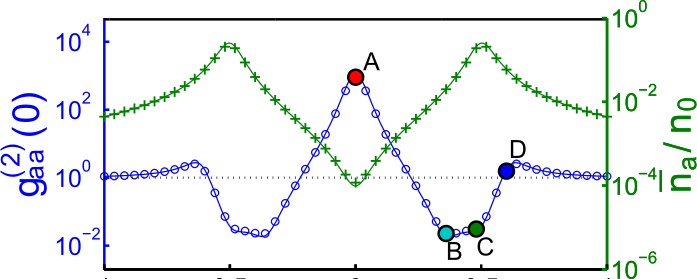
\includegraphics[width=0.45\textwidth]{./figs_Komar2013/fig2a.pdf}\quad
%   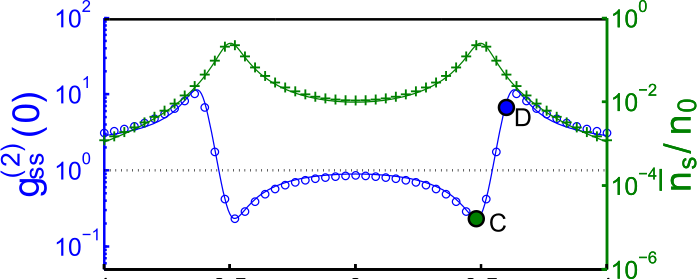
\includegraphics[width=0.45\textwidth]{./figs_Komar2013/fig2b.pdf}\\
%   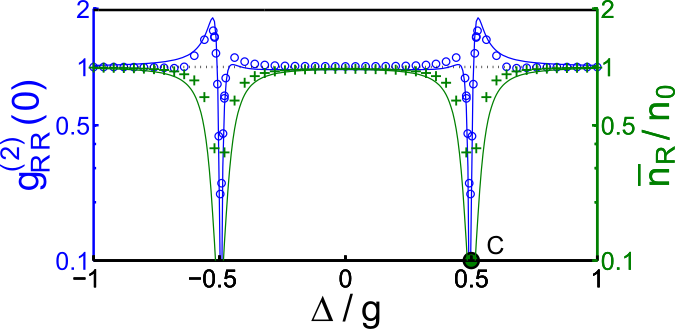
\includegraphics[width=0.45\textwidth]{./figs_Komar2013/fig2c.pdf}\quad
%   \includegraphics[width=0.45\textwidth]{./figs_Komar2013/fig2d.pdf}
%   \caption{
%   \label{fig:spectrum}(Color online)
%   (a) Normalized average photon number (green ``$+$")
%   and photon-photon correlation function (blue ``$\circ$")
%   for driven mode $c_a$
%   as a function of laser detuning at zero temperature.
%   Solid lines are calculated from analytic model
%   (see Eqs.~(\ref{eq:na}-\ref{eq:g2AA}))
%   and points show full numerical calculation.
%   The average photon number is
%   normalized by $n_0 = (\Omega/\kappa)^2$.
%   (b) Same as in (a) for the undriven mode $c_s$,
%   and
%   (c) for the reflected field $c_R$.
%   In all plots we took
%    $g/\kappa = 20$ and $\gamma/\kappa$ = 0.2.
%   Dots mark features seen at values of
%   detuning $\Delta/g = 0 \mathrm{ (A)}, \frac{1}{\sqrt{8}} \mathrm{ (B)},
%   \frac{1}{2} \mathrm{ (C)}$ and  $\frac{\sqrt{6}}{4} \mathrm{ (D)}$. 
%   The
%   small discrepancy between the analytic and numerical results
%   in (c) is due to the approximation
%   $g/\kappa \gg 1$   to  
%   simplify the expressions in Eqs.~(\ref{eq:na}-\ref{eq:g2AA}).
%   Bottom panels A-D illustrate the origin of these features as explained in the text.
%   Suppression  (enhancement) of the
%   steady state population of a specific level is
%   indicated by a red X (green circle).
%   }
% \end{figure}
% ==================================

\begin{figure}
\centering
  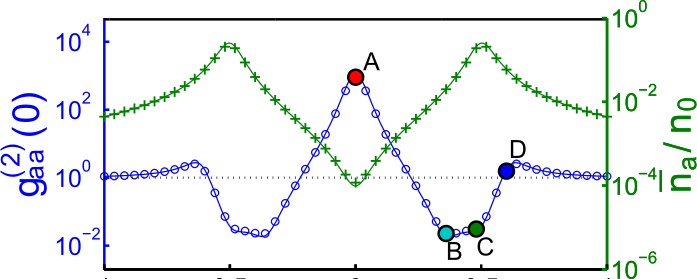
\includegraphics[width=0.8\textwidth]{./figs_Komar2013/fig2a.pdf}
  
  \caption
  [Photon statistics in anti-symmetric mode, $a$]
  {
  \label{fig:spectrum_a}
  Normalized average photon number (green ``$+$")
  and photon-photon correlation function (blue ``$\circ$")
  for driven mode $c_a$
  as a function of laser detuning at zero temperature.
  Solid lines are calculated from analytic model
  (see Eqs.~(\ref{eq:na}-\ref{eq:g2AA}))
  and points show full numerical calculation.
  The average photon number is
  normalized by $n_0 = (\Omega/\kappa)^2$. ($g/\kappa = 20$ and $\gamma/\kappa$
  = 0.2)
  }
\end{figure}

\begin{figure}
\centering
  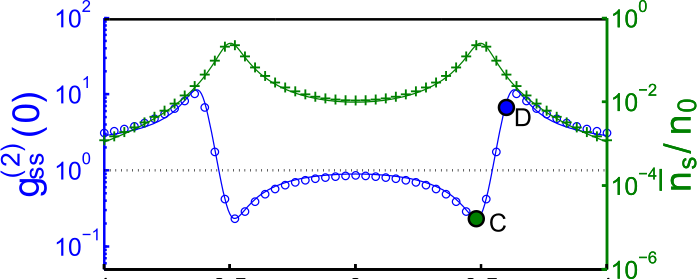
\includegraphics[width=0.8\textwidth]{./figs_Komar2013/fig2b.pdf}
  \caption
  [Photon statistics in symmetric mode, $s$]
  {
  \label{fig:spectrum_b}
  Normalized average photon number (green ``$+$")
  and photon-photon correlation function (blue ``$\circ$")
  for the undriven mode $c_s$
  as a function of laser detuning at zero temperature.
  Solid lines are calculated from analytic model
  (see Eqs.~(\ref{eq:na}-\ref{eq:g2AA}))
  and points show full numerical calculation.
  The average photon number is
  normalized by $n_0 = (\Omega/\kappa)^2$. ($g/\kappa = 20$ and $\gamma/\kappa$
  = 0.2)
  }
\end{figure}
 
\begin{figure}
\centering
  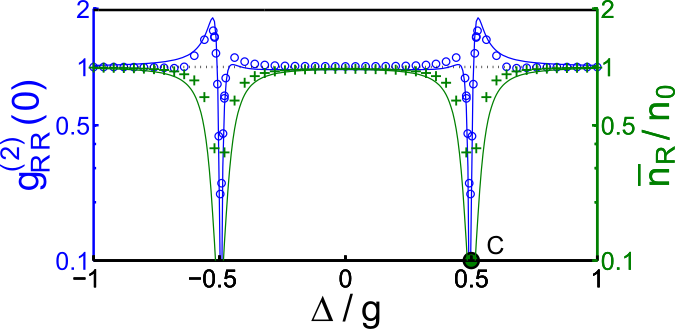
\includegraphics[width=0.8\textwidth]{./figs_Komar2013/fig2c.pdf}
  \caption
  [Photon statistics in reflected mode, $R$]
  {
  \label{fig:spectrum_c}
  Normalized average photon number (green ``$+$")
  and photon-photon correlation function (blue ``$\circ$")
  for the reflected field $c_R$,
  as a function of laser detuning at zero temperature.
  Solid lines are calculated from analytic model
  (see Eqs.~(\ref{eq:na}-\ref{eq:g2AA}))
  and points show full numerical calculation.
  The average photon number is
  normalized by $n_0 = (\Omega/\kappa)^2$.
  The
  small discrepancy between the analytic and numerical results is due to the
  approximation $g/\kappa \gg 1$   to  
  simplify the expressions in Eqs.~(\ref{eq:na}-\ref{eq:g2AA})
  ($g/\kappa = 20$ and $\gamma/\kappa$ = 0.2)
  }
\end{figure}
 


In addition to the transmission,
we plot the mean reflected photon number
in  \reffig{fig:spectrum_c}.
As discussed below, the reflected 
photon statistics
can also exhibit signatures of
nonlinearity.
We  calculate properties of the reflected light
using the
annihilation operator 
$c_R = c_a + i\frac{\Omega}{\kappa}$, obtained from standard input-output relations
for a symmetric two-sided cavity (see Appendix
\ref{App: Reflection}).
%$c_R = c_a + i\frac{\Omega}{\kappa}$.
The mean reflected photon number
$\bar n_R = \ev{c_R\+ c_R}$
is plotted in \reffig{fig:spectrum_c}.
%shows the reflected photon number, 
%$\bar n_R = \ev{c_R\+ c_R}$. 
At $\Delta/g = \pm \frac{1}{2}$, 
the average reflection has a minimum where the
average transmission has a maximum. 
Note that in contrast to a single cavity, 
even on resonance the transmission probability
is less than unity and the reflection probability
remains finite.



\subsection{Intensity correlations}
\label{sec:onetime_correlation}

To  characterize nonclassical 
photon statistics in the light transmitted through the OMS,
we study the equal-time photon-photon correlation
functions,
\bel
	\label{eq:g2(0)}
	g^{(2)}_{ii}(0)
	= \frac{\ev{c_i\+ c_i\+
	c_i  c_i }}{\ev{c_i\+ c_i}^2} ,
\eel
where all operators are evaluated at the same time and $i = a,s, R$. 
A normalized correlation of
$g^{(2)}_{ii}(0)< 1$ indicates photon anti-bunching, and the limit
$g^{(2)}_{ii}(0)\rightarrow 0$ corresponds to the 
complete photon blockade regime
in which two photons never occupy the cavity
at the same time.
The solid curves show $g^{(2)}_{aa}(0)$ in \reffig{fig:spectrum_a},
$g^{(2)}_{ss}(0)$ in \reffig{fig:spectrum_b} and $g^{(2)}_{RR}(0)$ 
\reffig{fig:spectrum_c} as a function of the laser  detuning and in the limit of
weak driving $\Omega/\kappa \ll1 $.
%for modes $c_a$, $c_s$ and the reflected
%mode $c_R$, respectively.
The most pronounced features of these correlation functions occur at 
$|\Delta|/g = 0, \frac{1}{\sqrt{8}}, \frac{1}{2} \mathrm{ and }\frac{\sqrt{6}}{4}$, 
as marked by
dots A, B, C and D, respectively. 
As we explain in detail in the following analysis, 
%Fig.~\ref{fig:spectrum}, 
we find that the photon bunching at A and
anti-bunching at B are the result of destructive 
quantum interference, while the 
features at points C and D arise from 
one- and two-photon resonances. 

%As illustrated in the bottom panel of
%Fig.~\ref{fig:spectrum}, 
%the photon bunching at A and
%anti-bunching at B arise from the suppression 
%of populations in states
%$|100\rangle$ and $|200\rangle$ respectively,
%due to destructive quantum interference
%(depicted by a red X).
%In contrast, the features at points C and D arise from 
%one- and two-photon
%resonances of the coupled system (indicated by a green O).
%These features can be understood
%in terms of a simple analytic model as we now discuss.

To gain insight into the two photon correlation functions shown in 
%We can capture the 
%features in  
\reffig{fig:spectrum_a}, \ref{fig:spectrum_b} and \ref{fig:spectrum_c},
we develop  an approximate analytic model 
for the system 
by considering only the
six levels shown in \reffig{fig:cartoon_b}.
Assuming that the system is initially prepared in $|000\rangle$, these are
the only levels significantly populated by weakly driving the
$c_a$ mode. We make the ansatz \cite{Carmichael1991}
\bel
\label{eq:psi}
\begin{split}
	\ket{\psi} =&\quad A_{000}\ket{000} + A_{100}\ket{100} + A_{011}\ket{011}\\
	&+ A_{200} \ket{200} + A_{111} \ket{111} + A_{022} \ket{022},
\end{split}
\eel
and describe the dynamics by evolving $|\psi\rangle$ under the action of the
non-Hermitian Hamiltonian, $\tilde{H} = H -i\left[\kappa c_a\+ c_a + \kappa
c_s\+ c_s + \frac{\gamma}{2} b\+ b\right]$. 
This approach allows us to evaluate
intensities up to order $\Omega^2$ and two-point correlation up to order
$\Omega^4$, since the neglected quantum jumps
lead to higher order corrections.
By neglecting the typically small mechanical decay rate
$\gamma \ll \kappa$,
the amplitudes in \refeq{eq:psi} then satisfy
\bal
	\label{eq:c000}\dot A_{000} &=& 0,\\[0.2cm]
	\dot A_{100} &=& -i\frac{g}{2} A_{011} -i\Omega A_{000} -
	\tilde\kappa A_{100},\\
	\label{eq:c011}
	\dot A_{011} &=& -i\frac{g}{2} A_{100} - \tilde\kappa A_{011},\\[0.2cm]
	\dot A_{200} &=& -i\frac{g}{\sqrt{2}} A_{111} -i\sqrt{2}\Omega A_{100}
	-2\tilde\kappa A_{200},\\
	\dot A_{111} &=& -i\frac{g}{\sqrt{2}} A_{200} -ig A_{022} - i\Omega A_{011} -
	2\tilde\kappa A_{111},\\
	\label{eq:c022}
	\dot A_{022} &=& -ig A_{111} -2\tilde\kappa A_{022},
\eal
where $\tilde \kappa = \kappa -i\Delta$. 
It is straightforward to solve
Eqs. (\ref{eq:c000}--\ref{eq:c022}) for the steady state amplitudes 
(see Appendix \ref{sect:App:steady_state}).
%\ref{sect:App:steady_state}
To lowest order in $\Omega/\kappa$  the mean
occupation numbers are $\bar n_a=|\bar A_{100}|^2$, $\bar n_s=|\bar A_{011}|^2$
and $\bar n_R=|\bar A_{100}+i\Omega/\kappa|^2$, where $\bar A$ denote
steady state amplitudes. We obtain
\bal
	\label{eq:na}
	\frac{\bar n_a}{n_0} &=&
		\frac{
			\kappa^2\left[R_\kappa(0)\right]^{1/2}
		}
		{
			R_\kappa\left(\frac{g}{2}\right)
		},\\
	\frac{\bar n_s}{n_0} &=&
		\frac{
			g^2\kappa^2
		}
		{
			4R_\kappa\left(\frac{g}{2}\right)
		},\\
	\frac{\bar n_R}{n_0} &\approx &
		\frac{
			\left[R_{\kappa/2}\left(\frac{g}{2}\right)\right]^2
		}
		{
			\left[R_\kappa\left(\frac{g}{2}\right)\right]^2
		},
\eal
where 
$R_K(\omega) = \left[K^2 +
(\Delta-\omega)^2\right]\left[K^2 + (\Delta+\omega)^2\right]$
and
$n_0 = (\Omega/\kappa)^2$.
%and $R_K(\omega) = \left[K^2 +
%(\Delta-\omega)^2\right]\left[K^2 + (\Delta+\omega)^2\right]$. 
From the 
factors $R_K(\omega)$ in the denominators  (numerators)
in these expressions, we obtain the positions
of the resonances  (antiresonances) in the 
average intracavity photon numbers, in excellent
agreement with the numerical results
shown in \reffig{fig:spectrum_a}, \ref{fig:spectrum_b} and
\ref{fig:spectrum_c}.
%We discuss these features in  detail below.
Our six-level model also provides the
equal-time correlations
(see Appendix \ref{sect:App:steady_state}),
%for
%which we find (see Appendix)
%\ref{sect:App:steady_state})
\bal
	g^{(2)}_{aa}(0) &=&
		\frac{
			R_\kappa\left(\frac{g}{\sqrt{8}}\right)
			R_\kappa\left(\frac{g}{2}\right)
		}
		{
			R_\kappa(0)
			R_\kappa\left(\frac{\sqrt{6}}{4}g\right)
		},
		\label{eq:g2aa}
		\\
	g^{(2)}_{ss}(0) &=&
		\frac{ 2
			R_\kappa\left(\frac{g}{2}\right)
		}
		{
			R_\kappa\left(\frac{\sqrt{6}}{4}g\right)
		},\\
	g^{(2)}_{RR}(0) &\approx &
		\frac{
			R_\kappa\left(\frac{g}{2}\right)
			R_{16\kappa^3/g^2}\left(\frac{g}{2}-\frac{2\kappa^2}{g}\right)
		}
		{
			\left[R_{\kappa/2}\left(\frac{g}{2}\right)\right]^2
		}.
		\label{eq:g2AA}
\eal
Again, these expressions are in agreement with
the features seen in the numerical results in \reffig{fig:spectrum_a},
\ref{fig:spectrum_b} and \ref{fig:spectrum_c}.
The positions of maxima and minima are
seen directly by the arguments of
the factors $R_K(\omega)$. 
Note that we assumed $g/\kappa \gg 1$ to
obtain the simplified
expressions in Eqs.~(\ref{eq:g2aa}-\ref{eq:g2AA}),
but we retained the 
shift of order $g (\kappa / g)^2$ in
the argument in \refeq{eq:g2AA}
%in the argument of the second $R$ symbol,
because this shift is larger than the width of 
the antiresonance.

%we approximated
%\refeq{eq:g2AA}, 


%To gain further insight on the positions of 
%the features seen in \reffig{fig:spectrum}
%and described by Eqs.~(\ref{eq:na}--\ref{eq:g2AA}), we 
%diagonalize $H$ in \refeq{eq:Hamiltonian_0} in the
%six-level subspace of \refeq{eq:psi}.
%This yields the following eigenstates (see
%\reffig{fig:cartoon}(b)):
%\bal
%	\label{eq:ket 0}\ket{0} &=& \ket{000},
%	\\
%	\label{eq:ket 1pm}\ket{1_\pm} &=& \frac{1}{\sqrt{2}}\left(\ket{100} \pm
%	\ket{011}\right),
%	\\
%	\label{eq:ket 2pm}\ket{2_\pm} &=& \frac{1}{\sqrt{6}}\left(\ket{200}\pm
%	\sqrt{3}\ket{111} + \sqrt{2}\ket{022}\right), 
%	\\
%	\label{eq:ket 2 0}\ket{2_0} &=& \frac{1}{\sqrt{3}}\left(\sqrt{2}\ket{200} -
%	\ket{022}\right).
%\eal
%In the diagonal basis, the weak drive couples all levels with total photon
%number $n$ to all levels with $n\pm 1$ photons.
%Some of the features arise simply from detuning
%the drive through one- or two-photon resonance
%with these eigenstates of the coupled OM system.

\begin{figure}
\centering
  \includegraphics[width=0.9\textwidth]{./figs_Komar2013/fig2d.pdf}
  \caption
  [Illustration of dominant processes]
  {
  \label{fig:spectrum_d}
  Illustration of the origin of the features marked with A,B,C and D on
  \reffig{fig:spectrum_a}, \ref{fig:spectrum_b} and \ref{fig:spectrum_c} as
  explained in the text.
  Suppression  (enhancement) of the
  steady state population of a specific level is
  indicated by a red X (green circle).
  }
\end{figure}
We now discuss each feature
in \reffig{fig:spectrum_a}, \ref{fig:spectrum_b} and \ref{fig:spectrum_c} in
terms of our six-level model together with the diagonal basis
in Eqs.~(\ref{eq:ket0}-\ref{eq:ket20}).
First, at 
detuning $\Delta = 0$ (point A in \reffig{fig:spectrum_a})
we see $g^{(2)}_{aa}(0)>1$, indicating bunching.  
This is due to destructive interference that
suppresses
the population in  $\ket{100}$ 
(panel A in \reffig{fig:spectrum_d}), and
can be understood as the system being
driven into a dark state,
$\ket{d} \propto g \ket{000} - \Omega \ket{011}$, similar to
electromagnetically induced 
transparency (EIT) \cite{Lukin2003, Weis2010}.
In the dark state, $\ket{011}$ remains populated,
% KS: I changed 110 -> 100 here
% SB: both incorrect, should be 011 
%by the weak drive, 
allowing transitions to $\ket{111}$
which in turn is strongly coupled to
$\ket{200}$.
The net result is a relative 
suppression of the probability to have one photon
compared to two photons
in the driven mode, 
leading to bunching at $\Delta = 0$.
Second, at detuning $\Delta = g/\sqrt{8}$ 
(point B), 
mode $c_a$ shows anti-bunching
due to a suppressed two-photon probability.
Again, this is due to destructive interference, or
the presence of a dark state in which
$\ket{200}$ remains unpopulated
(panel B).
Third, at detuning $\Delta = \frac{g}{2}$ 
(point C), 
all  modes show anti-bunching.
This is due to
a one-photon  resonant transition
$\ket{0} \rightarrow \ket{1_+}$ 
(panel C).
Finally, at detuning $\Delta = \frac{\sqrt{6}}{4}g$ 
(point D), 
both $c_a$ and $c_s$ show bunching due
to a two-photon resonant transition
$\ket{0} \rightarrow \ket{2_+}$
(panel D).
% KS: I replaced cartoon -> inset
% SB: inset -> panel



\subsection{Absence of two-photon resonance at $\Delta = 0$}

At first glance,
the level diagram in \reffig{fig:cartoon_b} together with
bunching 
in \reffig{fig:spectrum_a} 
suggest a two-photon resonance
at zero detuning $\Delta = 0$,
where the energy of the
eigenstate $\ket{2_0}$ is equal to the energy of two drive photons.
However, 
as discussed above,
the bunching at $\Delta = 0$ arises 
entirely from
the suppression of a one-photon population;
further, we 
find that the expected two-photon resonance is 
cancelled by  interference.
This can be seen from a second order perturbative 
calculation of the two-photon Rabi frequency $\Omega_{0,2_0}^{(2)}$ for the transition 
$|0\rangle\rightarrow |2_0\rangle$.  
The two-photon state $\ket{2_0}$ can be
populated by the drive 
$H_{\rm dr} = \Omega (c_a^\dag + c_a)$ 
from state $\ket{0}$ 
via two intermediate one-photon
eigenstates, $\ket{1_\pm}$ given by \refeq{eq:ket1pm},
with energies $\omega_{1_\pm} = -\Delta \pm \frac{g}{2}$
in the rotating frame.
The resulting Rabi frequency is
\bel
\label{eq:fgr}
	\Omega_{0,2_0}^{(2)} = \sum_{n=1_-, 1_+}
\frac{\ev{2_0| H_{\rm dr} |n}\ev{n| H_{\rm dr} |0}}{\omega_n},
\eel
which vanishes at $\Delta=0$ 
%the two-photon Rabi frequency vanishes
as a consequence of destructive interference between the two amplitudes. 
The exact cancellation is lifted
by including finite dissipation and the full spectrum;
%leading to finite population in $\ket{2_0}$;
nonetheless this simple argument shows that
the expected two-photon resonance at $\Delta = 0$
is strongly 
suppressed.


%$\kappa$ or $\gamma$ the exact cancellation is lifted, 
%and
%the resulting small, but finite population in $|2_0\rangle$ is responsible for
%the antibunching in point A.


%This can be seen from a second order 
%Fermi's golden rule calculation.
%The two-photon state $\ket{2_0}$ can be
%populated by the driving field from state $\ket{0}$ 
%via  two intermediate one-photon
%eigenstates, $\ket{1_+}$ and $\ket{1_-}$. 
%The total transition rate is
%$\Gamma_{\ket{0}\rightarrow \ket{2_0}} = 2\pi \left| M \right|^2
%\delta\left(\omega_0 - \omega_{2_0} \right)$,
%where in the rotating frame
%$\omega_0 = \omega_{2_0} = 0$, $\omega_{1_\pm} = -\Delta \pm \frac{g}{2}$,
%and 
%\bel
%\label{eq:fgr}
%	M = \sum_{n=1_-, 1_+}
%\frac{\ev{2_0| H_{\rm dr} |n}\ev{n| H_{\rm dr} |0}}{\omega_n} = 0.
%\eel
%We see that on resonance,
%$\Delta = 0$, the total rate vanishes
%%$\Gamma_{\ket{0}\rightarrow \ket{2_0}}=0$.
%%This is a consequence of 
%due to
%destructive interference of
%the two-photon
%amplitudes that would allow the transition.
%\sdb{Fix this.}
%Of course, for non-zero $\kappa$ or $\gamma$ this exact interference is lifted, and the resulting small, but finite population in $|2_0\rangle$ is responsible for the antibunching in point A.  



%This can be seen from a second order perturbative calculation of the two photon Rabi frequency $\Omega_{0,2_0}^{(2)}$ for the transition 
%$|0\rangle\rightarrow |2_0\rangle$.  The two-photon state $\ket{2_0}$ can be
%populated by the driving field from state $\ket{0}$ 
%via  two intermediate one-photon
%eigenstates, $\ket{1_+}$ and $\ket{1_-}$, which in the rotating frame
%have energies $\omega_{1_\pm} = -\Delta \pm \frac{g}{2}$, respectively. 
%Therefore, 
%\bel
%\label{eq:fgr}
%	\Omega_{0,2_0}^{(2)} = \sum_{n=1_-, 1_+}
%\frac{\ev{2_0| H_{\rm dr} |n}\ev{n| H_{\rm dr} |0}}{\omega_n},
%\eel
%and we see that on resonance $\Delta=0$ the two-photon Rabi-frequency vanishes as a consequence of destructive interference between the two amplitudes. Of course, for non-zero $\kappa$ or $\gamma$ this exact interference is lifted, and the resulting small, but finite population in $|2_0\rangle$ is responsible for the antibunching in point A.  



Further evidence of the absence of a
two-photon resonance at $\Delta=0$ is
the lack of bunching in the undriven mode in  
\reffig{fig:spectrum_b}.
If there were a two-photon resonance,
one would expect that bunching
should also occur in the undriven mode,
since the state $\ket{2_0}$ involves both $c_a$
and $c_s$ modes. 
This is indeed the case
at detuning $\Delta = \frac{\sqrt{6}}{4} g$
(see point D in \reffig{fig:spectrum_b}),
where
both modes show bunching as a result of
two-photon resonance.
In contrast, we see  no bunching in
the undriven mode at $\Delta = 0$. 
%due to the
%cancellation of two-photon resonance by interference.
This supports our conclusion that the observed
bunching at $\Delta=0$ arises 
from suppression of 
population in $\ket{100}$ due to interference,
as discussed in Section \ref{sec:onetime_correlation},
and not from two-photon resonance.
%Instead, this bunching arises
%from a suppression of the one-photon amplitude
%$A_{100}$
%as discussed in Section \ref{sec:onetime_correlation}.
As discussed above, this interference
does not suppress population in 
$\ket{011}$,
so we do not expect
bunching in the $c_s$ mode from this effect.
% ==================================
\begin{figure} 
\centering
  \includegraphics[width=0.8\textwidth]{./figs_Komar2013/fig3.pdf}
  \caption
  [Aggregate photon statistics]
  {
  \label{fig:populations}
  Average number (green dashed) and intensity correlation
  (blue solid)
  of total photon number in the coupled OM system.
  Parameters are the same as in \reffig{fig:spectrum_a},
  and dots mark the same detunings.
  One- and two-photon resonances are
  seen at C and D,
  but we see no bunching in the
  total photon number at 
  $\Delta = 0$ (point A).
%  is where a two-photon transition
%  $\ket{0}\rightarrow\ket{2_0}$ is naively expected.
  This reflects the lack
  of two-photon resonance due to 
  destructive interference (see \refeq{eq:fgr}).  } 
\end{figure}
% ==================================

Finally, to confirm our intuitive picture we plot the
intensity correlation function, 
$g^{(2)}_{\mathrm{tot}}(0) =
\ev{n_{\mathrm{tot}}(n_{\mathrm{tot}}-1)}/\ev{n_{\mathrm{tot}}}^2$,
of the total photon number, $n_{\mathrm{tot}} = n_a +
n_s$,
in the coupled OM system in
\reffig{fig:populations}. 
The probability to find one photon in the combined
cavity is maximal at $\Delta/g=\pm \frac{1}{2}$ 
due to one-photon resonance.
Similarly, we  
observe antibunching at point C
and bunching at point D,
due  to interference and two-photon resonance
respectively,
as discussed 
in Section \ref{sec:onetime_correlation}.
%The two-photon probability also has a peak at $\Delta/g=\pm \frac{1}{2}$, since
%a second photon can enter the cavity off-resonantly.
%In addition, the two-photon probability has peaks at 
%$\Delta / g  = \pm \sqrt{6} /4$ due to two-photon resonances.  
However, we find neither bunching nor antibunching
at $\Delta = 0$, 
demonstrating the absence of a two-photon resonance
despite the fact that $\ket{2_0}$ lies at twice the
drive frequency.



%Finally, to confirm our intuitive picture we plot the
%total photon number and $g^{(2)}(0)$ in steady state in
%\reffig{fig:populations}.
%The number of photons ($n_\mathrm{tot} = n_a + n_s$) in the combined
%cavity is maximal and $g^{(2)}_\mathrm{tot}(0) =
%\ev{n_\mathrm{tot}(n_\mathrm{tot}-1)}/\ev{n_\mathrm{tot}}^2$
%is minimal at $\Delta/g=\pm \frac{1}{2}$ due to one-photon resonance causing anti-bunching.
%The $g^{(2)}_\mathrm{tot}(0)$ has peaks at 
%$\Delta / g  = \pm \sqrt{6} /4$ due to two-photon resonances.  
%However, there
%is no peak ($g^{(2)}_\mathrm{tot}(0) \approx 1$) at $\Delta = 0$, 
%demonstrating the absence of a two-photon resonance
%despite the fact that $\ket{2_0}$ lies at the twice the
%drive frequency.

 


\subsection{Finite temperature}

\begin{figure}
\centering
  \includegraphics[width=0.8\textwidth]{./figs_Komar2013/fig4a.pdf}
  \caption
  [Temperature dependence of the relevant levels]
  {
  \label{fig:thermal_g2_a}
  Level diagram showing the
  six states populated by the drive from level $|0,0,n\rangle$ (left), 
  and the associated
  eigenmodes (right) with $n$-dependent splittings.
}
\end{figure} 

\begin{figure}
\centering
  \includegraphics[width=0.8\textwidth]{./figs_Komar2013/fig4b.pdf}
  \caption
  [Effect of non-zero temperature on photon statistics of mode $a$]
  {
  \label{fig:thermal_g2_b}
  Driven mode correlation function $g^{(2)}_{aa}(0)$
  for thermal mechanical occupation $N_{\rm th} = 0,1,2$.
  Solid lines show the analytic calculation with $\gamma \rightarrow 0$,
   and  dots show the full numerical results for $N_{\rm th} = 2$ only.
  The inset shows the minimal $g^{(2)}_{aa}(0)$ as a function of $N_{\rm th}$ 
  for several
  coupling strengths. 
  Parameters are $g/\kappa=20$, and (for numerics) $\gamma/\kappa =  10^{-3}$.
}
\end{figure} 

\begin{figure}
\centering
  \includegraphics[width=0.8\textwidth]{./figs_Komar2013/fig4c.pdf}
  \caption
  [Effect of non-zero temperature on photon statistics of mode $s$]
  {
  \label{fig:thermal_g2_c}
  Undriven mode correlation function $g^{(2)}_{ss}(0)$
  for thermal mechanical occupation $N_{\rm th} = 0,1,2$.
  Solid lines show the analytic calculation with $\gamma \rightarrow 0$,
   and  dots show the full numerical results for $N_{\rm th} = 2$ only.
  The inset shows the minimal $g^{(2)}_{ss}(0)$ as a function of $N_{\rm th}$ 
  for several
  coupling strengths. 
  Parameters are $g/\kappa=20$, and (for numerics) $\gamma/\kappa =  10^{-3}$.
}
\end{figure} 


So far in our analysis
we have focused on the case where the mechanical
system is prepared in its vibrational 
ground state, $|0_m\rangle$. 
This
condition can be achieved using high frequency resonators 
operated at cryogenic
temperatures \cite{O'Connell2010}, 
and in the limit of weak driving $\Omega/\kappa\ll1$ such
that optical
heating of the mechanical mode can be neglected. 
The mechanical ground state  could also be 
prepared using OM cooling \cite{Metzger2004, Gigan2006, 
Arcizet2006, Kleckner2006, Corbitt2007, 
Schliesser2008,Thompson2008,Wilson2009,
O'Connell2010,Teufel2011,Chan2011},
using an optical mode far-detuned
from the ones we consider  here for 
nonlinear interactions
\cite{Stannigel2012}.
Nonetheless,
in the
following we extend our analytic treatment to the case of finite temperature, 
and show that many of the
nonclassical features are robust even
in the presence of small
but finite thermal occupation of the mechanical mode.


To generalize our previous results we now consider
a finite equilibrium occupation number $N_{\rm th} >0$ of 
the mechanical mode,
but still assume that $\gamma(N_{\rm th}+1) \ll\kappa,g$. 
Within this approximation we proceed
as above, and
make a similar six-level ansatz as in Eq.~\eqref{eq:psi}
for each phonon number $n$,
%\bel
%\label{eq:psi_thermal}
%\begin{split}
%	&\ket{\psi_n} =\\
%	&\quad A_{0,0,n}\ket{0,0,n} + A_{1,0,n}\ket{1,0,n} +
%	A_{0,1,n+1}\ket{0,1,n+1}\\
%	&+ A_{2,0,n} \ket{2,0,n} + A_{1,1,n+1} \ket{1,1,n+1} \\
%	&+ A_{0,2,n+2}\ket{0,2,n+2},
%\end{split}
%\eel
\bel
\label{eq:psi_thermal}
\begin{split}
	\ket{\psi_n} &=
	 A_{0,0,n}\ket{0,0,n} + A_{1,0,n}\ket{1,0,n} \\
	&+ A_{0,1,n+1}\ket{0,1,n+1} + A_{2,0,n} \ket{2,0,n} \\
	&+ A_{1,1,n+1} \ket{1,1,n+1} 
	+ A_{0,2,n+2}\ket{0,2,n+2},
\end{split}
\eel
 where $\ket{\psi_n}$ includes states up
 to two photons that are connected 
 by the weak drive and coupling $g$,
 starting from the state $|0 0 n\rangle$. 
 As
 shown in Fig.~\ref{fig:thermal_g2_a} the coupling between the states
 within each six-level subspace
 depends explicitly on the phonon number $n$. 
Following the same approach as above,
the amplitudes in Eq.~\eqref{eq:psi_thermal} evolve according to
\bal
       \dot A_{0,0,n} &=& 0,\\
\dot A_{1,0,n} &=& -i \frac{g}{2} \sqrt{n+1} A_{0,1, n+1} -i\Omega A_{,00,n}
-\tilde\kappa A_{1,0,n},\\
\dot A_{0,1,n+1} &=& -i\frac{g}{2} \sqrt{n+1} A_{1,0,n} - \tilde\kappa
A_{0,1,n+1},\\
\dot A_{2,0,0} &=& -i g\sqrt{\frac{n+1}{2}} A_{1,1,n+1} -i\sqrt{2}\Omega
A_{1,0,n}
-2 \tilde\kappa A_{2,0,n},\\
\dot A_{1,1,n+1} &=& -ig\sqrt{\frac{n+1}{2}}  A_{2,0,n} -i
g\sqrt{\frac{n+2}{2}}A_{0,2,n+2} - i\Omega A_{0,1,n+1} - 2\tilde\kappa
A_{1,1,n+1},\qquad \\
\dot A_{0,2,n+2} &=& -ig\sqrt{\frac{n+2}{2}} A_{1,1,n+1} -2\tilde\kappa
A_{0,2,n+2}.
\eal
We solve for the steady state amplitudes within each 
subspace  $n$ and average
the result over the initial thermal phonon distribution,
assuming no coupling between subspaces due to
the small phonon relaxation rate.
We obtain the
average photon numbers
\begin{align}
	\bar n_a=\sum_n \zeta_n |\bar A_{1,0,n}|^2,
	\qquad
	\bar n_s=\sum_n \zeta_n |\bar A_{0,1,n+1}|^2,
\end{align}
where $\zeta_n=e^{-\beta \hbar\omega_m n}(1-e^{-\beta \hbar\omega_m })$ and
$\beta^{-1}=k_B T$.
Similarly, the $g^{(2)}_{ii}(0)$ functions are given by 
\begin{align}
	g^{(2)}_{aa}(0)=&2\sum_n\zeta_n |\bar A_{2,0,n}|^2 / \bar n_a^2,\\
	g^{(2)}_{ss}(0)=&2\sum_n\zeta_n |\bar A_{0,2,n+2}|^2 / \bar n_s^2.
\end{align} 
We provide the expressions for the steady state amplitudes
$\bar A_{2,0,n}$ and $\bar A_{0,2,n+2}$ in the
 Appendix \ref{sect:App:steady_state}.

 





We plot the correlation functions,
$g^{(2)}_{aa}(0)$ in \reffig{fig:thermal_g2_b} and $g^{(2)}_{ss}(0)$ in
\reffig{fig:thermal_g2_c} for different thermal phonon numbers, $N_{\rm th}$. 
Solid lines were calculated from the above
analytic approach with $\gamma \rightarrow 0$, 
and we find excellent agreement with
the full numerical results including small but finite
$\gamma$ (dots, shown only for
thermal occupation $N_{\rm th} = 2$).
We see that the zero temperature
features such as antibunching
survive at finite temperature for sufficiently strong coupling~\cite{Stannigel2012}.
In the insets we plot the minimum antibunching
as a function of thermal occupation number for
several ratios $g / \kappa$. 
Antibunching remains visible up
to a critical thermal phonon number, 
set by $g/\kappa$, 
beyond which the contributions from 
different phonon numbers smear out the effect
and antibunching vanishes.
%\pk{This antibunching vanishes for $N_\mathrm{th}
%\sim g^2/\kappa^2$, which we can understand from estimating $\bar{n}_a
%\sim\frac{\Omega^2}{g^2}\left(\frac{g^2}{\kappa^2N_\mathrm{th}}+1\right)$, and the
%two photon probability $\sim\frac{\Omega^2}{g^2}\bar{n}_a$ at $\Delta = g/2$,
%for $g\gg \kappa$.} 
In addition, for detunings $|\Delta|>g/2$, a series of new
resonances appear in the correlation functions, 
and for small but finite occupation numbers we  find
new antibunching features that are absent for $N_{\rm th}=0$.
These new features  can be understood from the $n$-dependent splitting of the
one- and two-photon manifolds as indicated in \reffig{fig:thermal_g2_a}.
For higher temperatures the individual resonances start to overlap, and we
observe an overall increase over a broad region of large positive and negative
detunings due to the cumulative effect of different phonon numbers.
% % ==================================
% \begin{figure}
% \centering
%   \includegraphics[width=0.7\textwidth]{./figs_Komar2013/fig4a.pdf}\\
%   \includegraphics[width=0.7\textwidth]{./figs_Komar2013/fig4b.pdf}\\
%   \includegraphics[width=0.7\textwidth]{./figs_Komar2013/fig4c.pdf}
%   \caption{
%   \label{fig:thermal_g2}(Color online)
%   Correlation functions for finite temperature. (a) Level diagram showing the
%   six states populated by the drive from level $|0,0,n\rangle$ (left), 
%   and the associated
%   eigenmodes (right) with $n$-dependent splittings.
%   (b) Driven mode correlation function $g^{(2)}_{aa}(0)$
%   for thermal mechanical occupation $N_{\rm th} = 0,1,2$.
%   Solid lines show the analytic calculation with $\gamma \rightarrow 0$,
%    and  dots show the full numerical results for $N_{\rm th} = 2$ only.
%   The inset shows the minimal $g^{(2)}_{aa}(0)$ as a function of $N_{\rm th}$ 
%   for several
%   coupling strengths. 
%   (c) Same as (b) for the undriven mode correlation function $g^{(2)}_{ss}(0)$. 
%   Parameters are $g/\kappa=20$, and (for numerics) $\gamma/\kappa =  10^{-3}$.
% }
% \end{figure} 
% % ================================== 



%%%%%%%%%%%%%%%%%%%%%%%%%%%%%%%%%%%%%%%%
%%%%%%%%%%%%%%%%%%%%%%%%%%%%%%%%%%%%%%%%
\section{Delayed coincidence and single phonon states}
\label{sect:Delayed_coincidence}


In addition to the equal-time correlations discussed above,
quantum signatures can also be manifested in photon
intensity correlations with a finite time delay.
We now turn to a discussion of  delayed coincidence
characterized by the 
two-time
intensity correlations functions,
\bel
\label{eq:g2_tau}
	g^{(2)}_{ii}(\tau) = \frac{\ev{c_i\+(0) c_i\+ (\tau) c _i(\tau)
	c_i(0)}}{\ev{c_i\+ c_i}^2},
\eel
for both driven and undriven modes, $i = a,s$.
Expressing this correlation in terms of a classical
light intensity $I$,
$g^{(2)}(\tau) = \ev{ I(\tau) I(0) } / \ev{ I }^2$,
and
using the Schwarz inequality, we
obtain the inequalities \cite{Carmichael1991, Brecha1999},
\begin{align}
  \label{eq:classical_criterium}
 	g^{(2)}(\tau) &\leq g^{(2)}(0),	%\quad &(\mathrm{classical}),
	\\
	 |g^{(2)}(\tau)-1| & \leq |g^{(2)}(0)-1| .%\quad &(\mathrm{classical}),
\end{align}
Similar to the classical inequality
$g^{(2)}(0) > 1$ at zero delay, 
violation of either of these inequalities
at finite delay is
a signature of quantum light. 
We calculate the delayed coincidence correlation
functions
for both the driven and undriven modes.


\subsection{Driven mode}
The
correlation function $g^{(2)}_{aa}(\tau)$ is shown in \reffig{fig:g2aatau}(a)
for two values of the detuning $\Delta$.
The most striking feature
is the apparent vanishing of  $g^{(2)}_{aa}(\tau)$
at several values of $\tau$ when the
detuning is $\Delta = 0$ (curve A in \reffig{fig:g2aatau}(a)).
These are due to Rabi oscillations at frequency
$g/2$ following the detection of a photon.
This vanishing of the finite delay correlation function
is reminiscent of  wavefunction collapse that
occurs in a cavity containing an 
atomic ensemble \cite{Carmichael1991},
and while its origins are similar, there are important
differences as we now discuss.




We can understand the finite delay intensity
correlations
in terms of the simple six-level model discussed
in the previous section.
We extend
this model to describe finite delay correlations
by considering the effect of photodetection on
the steady state of the system.
Detection of a photon in the driven mode projects
the system onto the conditional state \cite{QuantumNoise},
\bel
	\label{eq:psi^a}
	\ket{\psi^a} = \frac{c_a \ket{\psi}}{||c_a \ket{\psi} ||},
\eel
where $\ket{\psi}$ is given by \refeq{eq:psi} with steady state amplitudes
and $|| \cdot ||$ denotes normalization after the jump.
The conditional state $\ket{\psi^a}$ has an {\it increased}
amplitude $A_{100}$ after the jump
(see jump at $\tau = 0$ in \reffig{fig:g2aatau} (b)).
Following this initial photodetection, the amplitude 
$A_{100}$
subsequently undergoes Rabi oscillations with frequency $g/2$,
and decays back to its steady state at rate $2\kappa$. 
For sufficiently large bunching at zero delay and
strong coupling $g > \kappa$, the  Rabi oscillations of the amplitude
$A_{100}(\tau)$ can cause it to cross zero 
several times before it decays back
to steady state.
As the probability to detect a second photon is dominated by $A_{100}$,
its zeros are responsible for the zeros in the correlation
function $g^{(2)}_{aa}(\tau)$ zero at these delay times.





The zeros in $g^{(2)}(\tau)$ appear similar
to those exhibited  in
a cavity strongly coupled to
an atomic ensemble \cite{Carmichael1991, Rice1988, Brecha1999} or a single atom
\cite{Chang2007}. 
However, in stark contrast to the atomic case,
the zeros in \reffig{fig:g2aatau}(a)
are the result of Rabi oscillations  following
the initial quantum jump.
This is qualitatively different from
the atomic case, where the change in
sign of the relevant amplitude (the analogy of $A_{100}$)
occurs {\it immediately} after the jump itself, and the amplitude
is damped back to steady state at the atomic
decay rate $\Gamma$, without Rabi oscillation. 
As a consequence, the vanishing correlation
function in the atomic case occurs
at a delay set by $\tau_0 \sim \gamma^{-1}\ln C$, 
requiring only strong cooperativity $C = g^2/ \kappa \gamma > 1$
to be visible.
On the other hand,
the zeros in \reffig{fig:g2aatau}(a)
occur at delay times set by  $\tau \sim 1/g$,
requiring strictly strong coupling $g > \kappa$.








Before moving on to correlations of the undriven mode,
we briefly discuss the correlations of the driven mode at the
 other value of  detuning shown in 
\reffig{fig:g2aatau}(a).
 At detuning
$\Delta = \frac{g}{\sqrt{2}}$ (curve E),
which shows bunching at zero time,
$g^{(2)}_{aa}(0) \gtrsim 1$, 
increases  above its initial value at
finite delay.
This is a violation of the classical inequality in
\refeq{eq:classical_criterium}, 
and is an example of ``delayed bunching,"
or an increased probability to detect a second
photon at a finite delay time.
A similar effect was recently studied
in a single mode OMS \cite{Kronwald2012}.
However, like the Rabi oscillations,
the increased correlation function decays back to its steady state
value of 1 on
the timescale of $\kappa^{-1}$.
%%%%%%%%%%%%%%%%%%%%%%%%%%%%%
%%%%%%%%%%%%%%%%%%%%%%%%%%%%%
\begin{figure} 
\centering
  \includegraphics[width=0.9\textwidth]{./figs_Komar2013/fig5a.pdf}\\[-0.5cm]
  \includegraphics[width=0.9\textwidth]{./figs_Komar2013/fig5b.pdf}
  \caption
  [Autocorrelation of mode $a$]
  {
  \label{fig:g2aatau}
  (a) Finite time delay intensity
  correlation function $g^{(2)}_{aa}(\tau)$  for detunings
  $\Delta/g = 0 \mathrm{ (A)}$ and $\frac{1}{\sqrt{2}}
  \mathrm{ (E)}$.
  Detuning for curve A is the same as marked in \reffig{fig:spectrum_a},
  while E shows a new effect not seen at equal times.
  Thin dashed line indicates the classical bound 
  (see \refeq{eq:classical_criterium}) for curve E. 
  (b) Evolution of amplitude $A_{100}$ (normalized by its
  steady state value)
  at detuning A, $\Delta/g = 0$,
  after detecting a driven $c_a$ photon at $\tau = 0$. 
  Vertical dash-dotted lines mark delay times ($\tau_1, \tau_2$) where this amplitude
  vanishes resulting in the vanishing of $g^{(2)}_{aa}(\tau)$
  in (a).
  Parameters are $g/\kappa = 8$ and $\gamma/\kappa$ = 0.02. 
  } 
\end{figure}
%%%%%%%%%%%%%%%%%%%%%%%%%%%%%
%%%%%%%%%%%%%%%%%%%%%%%%%%%%%




\subsection{Heralded single phonon states}

We now turn to a discussion of the delayed coincidence
correlations of the undriven mode $c_s$.
We note that correlations of the driven
and undriven modes can be measured separately
provided sufficient frequency resolution, smaller than
  the mechanical frequency.
The correlation function
$g^{(2)}_{ss}(\tau)$
of the undriven mode
is shown in \reffig{fig:g2sstau} for several
values of detuning.
Similar to the driven mode, the
correlation function of the undriven mode
exhibits Rabi oscillations 
that decay on the short optical
timescale
$1/\kappa$.
For detuning $\Delta = 0$ and 
$\Delta/g = \frac{\sqrt{6}}{4}$
(curves A and D in \reffig{fig:g2sstau}),
the correlation $g^{(2)}_{ss}(\tau)$
is described by
our previous six-level 
model of Eqs. (\ref{eq:c000}--\ref{eq:c022}).
However,  at detuning $\Delta = \frac{g}{\sqrt{2}}$
(curve E), we see that
$g^{(2)}_{ss}(\tau)$ has a long
tail that decays
on the much longer mechanical timescale $1/\gamma$.
This is due to the heralded preparation
of a single phonon by detection of a photon in the
undriven mode, as we now discuss.
%and can be understood
%by a simple extension of the six-level model
%discussed above.
%%%%%%%%%%%%%%%%%%%%%%%%%%%%%
%%%%%%%%%%%%%%%%%%%%%%%%%%%%% 
\begin{figure}[htb] \centering
  \includegraphics[width=0.8\textwidth]{./figs_Komar2013/fig6.pdf}
  \caption[Autocorrelation of mode $s$]
  { 
  \label{fig:g2sstau}
  Finite time delay intensity correlation function $g^{(2)}_{ss}(\tau)$
  for detunings $\Delta/g = 0 \mathrm{ (A)}, \sqrt{6}/4 \mathrm{ (D)}$
  and
  $\frac{1}{\sqrt{2}} \mathrm{ (E)}$.
  Thin dashed lines indicate the classical bounds
  (see  \refeq{eq:classical_criterium}).
  Labels A, D, E correspond to the same detunings
  marked in 
  \reffig{fig:spectrum_a}
  and
  \reffig{fig:g2aatau}.
  Parameters are $g/\kappa = 8$, and $\gamma/\kappa$ = 0.02.
  }
\end{figure}
%%%%%%%%%%%%%%%%%%%%%%%%%%%%%
%%%%%%%%%%%%%%%%%%%%%%%%%%%%%



The increase in delayed coincidence can be understood
by extending the above analytic six-level model to account
for the conditional state of the system after detection
of a photon in the undriven mode.
To do this,
we simply add three additional states to
the six-level ansatz in  \refeq{eq:psi},
\bel
\label{eq:psi9}
	\ket{\psi} = \dots + A_{001}\ket{001} + A_{101}\ket{101} + A_{012}\ket{012},
\eel
since these are the states populated by detection
of a $c_s$ photon from the original six states (see \reffig{fig:levels_jumps}).
Using the same 
%non-Hermitian dynamics
approach as before, we obtain the following equations for the
amplitudes,
\bal
	\label{eq:c001}
	\dot A_{001} &\approx& -\frac{\gamma}{2}A_{001},\\[0.2cm]
	\dot A_{101} &=& -i\frac{g}{\sqrt{2}} A_{012} -i\Omega A_{001} -
	\tilde\kappa A_{101},\\
	\label{eq:c012}
	\dot A_{012} &=& -i\frac{g}{\sqrt{2}} A_{101} - \tilde\kappa A_{012},
\eal
where we used $\gamma \ll \kappa$ and
kept the leading term in \refeq{eq:c001}.
We obtain $g^{(2)}_{ss}(\tau)$
by solving these equations for initial
conditions determined by the conditional state $\ket{\psi^s}$
after a quantum jump, 
\bel
	\label{eq:psi^s}
	\ket{\psi^s} = \frac{c_s \ket{\psi}}{||c_s \ket{\psi}||},
\eel
which is a superposition of states $\ket{001}, \ket{101}, \ket{012}$
(see Appendix \ref{sect:App:steady_state} 
%\ref{sect:two-time_analytic} 
for details), but in the limit of weak driving consist mainly of $|001\rangle$. 


Detection of a photon in the undriven mode
implies that the three-wave mixing interaction
converted a photon from the driven mode into
the undriven mode by simultaneously adding a phonon.
The relevant three-level subspace after the jump 
(see \reffig{fig:levels_jumps}) has a similar structure as in the steady state, 
but the presence of an extra phonon
modifies the splitting of the one-photon 
states $|1^\prime_{\pm}\rangle=(|101\rangle \pm |012\rangle)/\sqrt{2}$  to
$\frac{g}{\sqrt{2}}$ 
(instead of $g/2$ without a phonon).
%
%The increase in delayed coincidence
%at specific laser detuning is a direct consequence
%of this conversion,
%as illustrated in \reffig{fig:levels_jumps}.
%In steady state, the system occupies the
%six levels of \refeq{eq:psi}, shown 
%on the left in \reffig{fig:levels_jumps}.
%After detection of an undriven $c_s$ photon,
%the 
%emitted  phonon slowly decays back
%to its ground state at rate $\gamma$, 
%during which time the system is in the conditional
%subspace shown on the
%right in \reffig{fig:levels_jumps}.
%%%%%%%%%%%%%%%%%%%%%%%%%%%%%
%%%%%%%%%%%%%%%%%%%%%%%%%%%%% 
\begin{figure}[htb]
\centering  
  \includegraphics[width=0.85\textwidth]{./figs_Komar2013/fig7.pdf}\\
  \caption[Diagram of the metastable subspace]
  {
  \label{fig:levels_jumps}
  Effect of detection of a $c_s$ photon
  at detuning E ($\Delta/g = \frac{1}{\sqrt{2}}$).
  In steady state (gray region on left), 
  the drive is far off-resonant.
  However, after detection of a $c_s$ photon the system
  jumps into the conditional subspace (pink region on right).
  Due to the presence of an extra phonon in this subspace,
  the drive is resonant and the probability to detect a second
  photon is much higher than in steady state.
  This increased probability persists
  as long as the extra phonon,
  which decays slowly at rate $\gamma$.
  }
\end{figure}
%%%%%%%%%%%%%%%%%%%%%%%%%%%%%
%%%%%%%%%%%%%%%%%%%%%%%%%%%%%
This changes
the one-photon resonance condition
for the drive to $\Delta = \frac{g}{\sqrt{2}}$.
Therefore, at this value of the detuning,
the process of
exciting the system and emitting a single $c_s$ photon
is off-resonant;
while after the detection of a first $c_s$ photon
the system is prepared in $|001\rangle$, bringing
it into resonance with the drive.
%brings the system into resonance with the drive,
This {\it enhances}
the probability for subsequent excitation and emission
of a second $c_s$ photon, increasing
the correlation function at finite delay.
%successive excitation of the second photon 
%occurs exactly on resonance. 
%while 
%resonant in the presence of an extra phonon,
%such that 
%the probability to detect a second 
%photon 
%This process {\it enhances} the probability 
%of photon coincidences in the undriven mode, 
The maximum delayed coincidence
occurs after a delay of $\tau \sim 1/\kappa$,
when the photons have reached the
metastable steady state
in the conditional  subspace with one 
extra phonon.
Eventually, the delayed coincidence
returns to its true steady state value
of one
%of $g^{(2)}_{ss}(\tau) \rightarrow 1$
on the timescale
$\tau \sim 1/\gamma$, which is the mechanical decay time of the
state $|001\rangle$. 
%\pk{Detuning $\Delta/g = 1/\sqrt{2}$ is chosen in order
%to optimize the visibility of the long tail of $g^{(2)}_{ss}$. 
The long tails
observed for other values of detuning (curves A and D) are
also
due to the presence of an extra phonon,
but in these cases the system remains off-resonant
after the initial $c_s$ photon and the effect is less
 pronounced.
Note that the
probability  to detect a photon from the {\it driven} mode also increases in 
the conditional state, so a similar effect is seen in the delayed 
cross-correlation function $g^{(2)}_{as}(\tau)$, where the photon in the 
undriven mode is detected first.

%Detection of a photon in the undriven mode
%implies that the three-wave mixing interaction
%converted a photon in the driven mode into
%one in the undriven mode by generating a phonon.
%After this first detection, the 
%emitted single phonon slowly decays back
%to its ground state at rate $\gamma$.
%During this slow decay, the presence
%of the extra phonon modifies the resonance
%condition of the coupled OM system, 
%changing the probability to detect a second photon.
%Specifically, if the drive detuning is chosen so that the
%system is off-resonant in steady state
%(at zero temperature), but
%resonant in the presence of an extra phonon,
%then 
%the probability to detect a second 
%photon {\it increases}
%after detection of a photon in the undriven mode.
%This increase in the  coincidence correlation
%at finite delay seen in 
%$g^{(2)}_{ss}(\tau)$
%violates the classical inequality in
%\refeq{eq:classical_criterium}.



%%%%%%%%%%%%%%%%%%%%%%%%%%%%%%%%%%%%%%%%
%%%%%%%%%%%%%%%%%%%%%%%%%%%%%%%%%%%%%%%%
\section{Reaching strong coupling}
\label{sect:Experimental values}


The nonclassical correlations predicted in this chapter 
require  strong optomechanical coupling, $g > \kappa$, 
as well as sideband resolution, $\omega_m \gg \kappa,\gamma$. 
While the combination of these conditions has not 
yet been demonstrated, 
several experimental efforts 
%in OMSs 
are currently 
directed at reaching this regime. 
By using micro- and nano-fabricated OMSs such 
as microtoroids or photonic crystal beams, 
high frequency mechanical systems  with 
$\omega_m\approx 50$ MHz - 5 GHz can be combined 
with low loss optical modes, such that the 
condition $\omega_m \gg \kappa \gg \gamma$ is satisfied
\cite{Safavi-Naeini2011a, Schliesser2008, Eichenfield2009}.
At the same time the mechanical system can already 
be prepared close to the quantum ground state by working at cryogenic temperatures. 
In micro-fabricated OMSs, single-photon couplings of 
about $g/\kappa \approx 0.001$ have been demonstrated 
\cite{Eichenfield2009, Ding2011,Verhagen2011}
%\cite{Teufel2011,Teufel2011a}.
The largest value to date of $g/\kappa \approx 0.007$ 
has been reached in photonic crystal beam
resonators \cite{Chan2012}, where
colocalized optical and vibrational resonances are
highly confined to maximize coupling
while the surrounding structure is engineered  
to minimize loss.
Conversely, in cold atomic experiments
the effective strong OM coupling regime has been
reached \cite{Purdy2010}, while sideband resolution remains
a challenge \cite{Stamper-kurn}. 


%In experiments with a 
%micromechanical membrane capacitively coupled to
%a superconducting resonant microwave circuit,
%a ratio of $g/\kappa \approx 0.001$
%has been achieved \cite{Teufel2011,Teufel2011a}.
%The strongest
%ratio to date of ($g/\kappa \approx 0.005$) were 
%reached in photonic crystal beam
%resonators \cite{Chan2012}, where
%colocalized optical and vibrational resonances are
%highly confined to maximize coupling
%while the surrounding structure is engineered
%to minimize loss.
%However in systems with the highest achieved
%ratio of $g/\kappa$, two orders of magnitude
%improvement is required to reach
%the strong coupling
%regime. 


There are several existing
proposals for how to meet the challenge
of $g/\kappa > 1$ 
in the photonic crystal beam setup.
First, 
the single-photon optomechanical coupling can 
be increased by making use of
nanoslots in the structure \cite{Robinson2005, Davanc2012} 
to further localize the electric field at 
the position of the mechanical mode.
This could improve $g$ by a factor of 10
\cite{Ludwig2012}.
Second, numerical studies 
suggest that $\kappa$ can be further decreased
by fine tuning the size and position of the slots in
the photonic crystals \cite{Notomi2008,Tanaka2008}. 
Finally, new materials are currently being tested for an 
overall improvement of the OM properties of nano-fabricated devices
\cite{Xiong2012}.
Thus by using these ultrahigh $Q$ photonic crystals or 
similar designs, an increase of $g/\kappa$ by a factor of $\sim 100$ 
is realistic. 
Note that once the strong coupling condition has been achieved, 
the implementation of two or multimode OMSs 
with adjustable tunneling $2J\sim \omega_m$ can be realized via evanescent field
coupling, as has already been demonstrated in the weak coupling regime
\cite{Safavi-Naeini2011a, Eichenfield2009, Grudinin2010}.


%Implementing these
%proposals in experiment will clearly be challenging;
%however, we stress that 
%a two-mode approach can remove dependence upon the much larger
%mechanical frequency $\omega_m \gg \kappa$, making the realization of these
%feasible.




%%%%%%%%%%%%%%%%%%%%%%%%%%%%%%%%%%%%%%%%
%%%%%%%%%%%%%%%%%%%%%%%%%%%%%%%%%%%%%%%%
\section{Conclusions}
\label{sect:Conclusion}

We have studied  nonclassical intensity correlations in a
driven, near-resonant 
optomechanical system with  one mechanical and two optical modes.
In the regime of strong coupling $g > \kappa$, this system
allows for nonlinear quantum optics through a resonant three-mode 
interaction in which the exchange of two photons is mediated by a phonon.
We have identified several different processes
that can lead to nonclassical antibunching and delayed bunching, 
and we have  
derived a simple analytic model that allows us to 
describe and interpret photon-photon correlations in this 
system both at zero and at finite temperature. 
Our findings will be important as experiments
approach the regime of strong 
OM coupling, and for potential applications of 
OMSs for quantum information processing. 
%
%The requirement of strict strong coupling
%is in contrast to analogous atom-cavity
%systems, in which nonclassical correlations 
%persist in the less stringent regime of 
%strong cooperativity $g^2 > \kappa\gamma$.
%This is not surprising, since all states with appreciable population
%in steady state involve photons, which decay at rate $\kappa$.
%Nonetheless, 
In particular, the long-lived
correlation found for the undriven mode 
raises the intriguing possibility to
exploit such a setup as a quantum memory.
The generation of
heralded single phonons on detection
of a photon from the undriven mode may have implications
for building OM quantum 
repeaters and quantum communication devices.


%%%%%%%%%%%%%%%%%%%%%%%%%%%%%%%%%%%%%%%%
%%%%%%%%%%%%%%%%%%%%%%%%%%%%%%%%%%%%%%%%




 
% Chapter 3:
\chapter{Optomechanical quantum information processing with photons and phonons}
\label{ch:Stannigel2012}
%%%%%%%%%%%%%%%%%%%%%%%%%%%%%%%%%%%%%%%%%%%%%%%%

\section{Introduction}
From \cite{Stannigel2012}
 
% Chapter 4: 
\chapter{Heralded Quantum Gates with Integrated Error Detection in Optical Cavities}
\label{ch:Borregaard2015a}
%%%%%%%%%%%%%%%%%%%%%%%%%%%%%%%%%%%%%%%%%%%%%%%%

\section{Introduction}
From \cite{Borregaard2015a}

% Chapter 5:          
\chapter{Long-distance entanglement distribution using individual atoms in
optical cavities}
\label{ch:Borregaard2015b}
%%%%%%%%%%%%%%%%%%%%%%%%%%%%%%%%%%%%%%%%%%%%%%%%
 
\section{Introduction}
From \cite{Borregaard2015b}

% Chapter 6:  
\chapter{Heisenberg-Limited Atom Clocks Based on Entangled Qubits}
\label{ch:Kessler2014}
% From \cite{Kessler2014}
%%%%%%%%%%%%%%%%%%%%%%%%%%%%%%%%%%%%%%%%%%%%%%%%

%%%%%%%%%%%%%%%%%%%%%%%%%%%%%%%%%%%%%%%%%%%%%%%%%%%%%%%%%%%%%%%%%%%%%%%%%%%%%%%%%%5
%%%%%%%%%%%%%%%%%%%%%%%%%%%%%%%%%%%%%%%%%%%%%%%%%%%%%%%%%%%%%%%%%%%%%%%%%%%%%%%%%%5
\section{Introduction}
%%%%%%%%%%%%%%%%%%%%%%%%%%%%%%%%%%%%%%%%%%%%%%%%%%%%%%%%%%%%%%%%%%%%%%%%%%%%%%%%%%5
%%%%%%%%%%%%%%%%%%%%%%%%%%%%%%%%%%%%%%%%%%%%%%%%%%%%%%%%%%%%%%%%%%%%%%%%%%%%%%%%%%5
Currently, atomic clocks based on optical transitions achieve the most
precise \cite{Nicholson2012, Bloom2013, Lemke2009} and accurate \cite{Chou2010,
Bloom2013} frequency references.
Additionally, the development of optical frequency combs
\cite{Eckstein1978, Reichert2000, Jones2000, Ye2003} -- establishing a coherent
link between the optical and radio frequencies -- enabled the application
of optical frequency standards to a wide range of scientific and technological
fields including astronomy, molecular spectroscopy and global
positioning systems.

% The improvement of frequency standards using quantum resources, such as
% entanglement, has attracted wide attention in recent years \cite{Buzek1999,
% Andre2004, Rosenband2012, Rosenband2012_numerical}.

The improvement of frequency standards using quantum resources, such as
entanglement \cite{Buzek1999, Andre2004,LouchetChauvet:2010fs,Rosenband2012_numerical,
Borregaard2013_nearHeisenberg},
%, as well as
%schemes consiting of multi-layered interrogation and feedback
%\cite{Rosenband2013, Borregaard2013} 
has been actively explored in recent years. While clock protocols
based on uncorrelated atoms at best achieve a stability scaling
$\propto1/\sqrt{N}$, where $N$ is the number of atoms -- a
scaling commonly known as the standard quantum limit (SQL) \cite{Caves1980} --
the use of entangled resources, in principle, allows one to surpass this limit.
However, a characterization of the improvement obtainable by using entanglement
 requires a detailed investigation of the decoherence present in the system.
 Previous studies have focused on two kind of noise sources: i) single particle
 decoherence resulting from the interaction of the atoms with the environment
 and ii) frequency fluctuations in the laser used to excite the clock transition
 [in the following also referred to as local oscillator (LO)].
  It is well known that fully entangled states (e.g.,
  Greenberger-Horne-Zeilinger (GHZ) states) allow for improved spectroscopic sensitivity, but in the same way
 that these states benefit from their increased sensitivity in the laser
 interrogation, they are generally prone to various types of noise sources
 canceling any quantum gain. It has therefore been long believed that such
 states fail to increase clock stability regardless of the noise model being used
 \cite{Bollinger1996, Wineland1998, Rosenband2012_numerical,Huelga1997}. On the other hand, it has been shown that
for clocks with local oscillator noise limited stability, the use of
moderately squeezed atomic states can yield a modest improvement over the SQL
\cite{Andre2004,LouchetChauvet:2010fs}.
 A recent study demonstrated further that, in principle, highly squeezed states
could achieve Heisenberg-limited stability (i.e., a $1/N$ scaling
with the available resources representing the ultimate limit allowed by the laws
of quantum mechanics \cite{Giovanetti2011}) using a complex adaptive
measurement scheme \cite{Borregaard2013_nearHeisenberg}.
 At the same time, it has been shown that the single particle
 decoherence-limited regime can be reached for long averaging time at
a logarithmic cost in $N$ by interrogating uncorrelated atomic
ensembles for suitably chosen times \cite{Rosenband2013, Borregaard2013}.

In this chapter, we  introduce a protocol involving groups of sequentially
larger GHZ states to estimate local oscillator deviations from the atomic reference in
a manner reminiscent of the phase estimation algorithm \cite{Nielsen_Chuang}.
Furthermore, we unify previous treatments of decoherence for atomic clocks 
and incorporate previous proposals involving uncorrelated atoms to
effectively narrow the LO linewidth \cite{Rosenband2013, Borregaard2013} and thereby identify
 ultimate limits to the stability of atomic clocks based on entangled atoms. We find that for LO-noise limited clocks, the
proposed quantum protocol is found to be nearly optimal, realizing the
Heisenberg limit of clock stability up to a logarithmic correction in the
particle number.
Importantly, it reaches the fundamental noise floor  resulting from
individual dephasing of the clock qubits $N$ times faster than the best known
classical schemes, where $N$ is the total number of particles employed.

%In this Letter, we demonstrate that if the dominating noise is LO noise -- as it is the case in modern atomic clocks -- this limitation can be overcome.  
%As the LO fluctuations affect all clock atoms alike, this perfectly correlated noise does not represent a fundamental limitation in the interrogation process, and can be corrected for in a non-adaptive protocol based on multiple GHZ states of varying size, reminiscent of the phase estimation algorithm  \cite{Nielsen_Chuang}. 
%% The procedure is based on the
%% division of the available clock atoms into successively smaller GHZ groups
%% evolving at different phase velocities during the laser interrogation time. Each
%% GHZ group hereby keeps track of the accumulated phase slips of the next
%% ensemble, thus largely eliminating the problem of uncontrolled slips of the
%% laser phase. This allows us to operate a large part of the available resources
%% in a fully entangled state, reaching near-Heisenberg-limited spectroscopy for
%% LO-noise-limited optical clocks,  with an $\mathcal O(\sqrt N/ \mathrmrm{log}(N))$
%% stability improvement over the SQL. 
%We provide the full quantum mechanical
%derivation of this result, 
%% in a feedback analysis, 
%taking into account all relevant noise sources and optimizing over all free
%parameters of the scheme.
%We investigate the limiting factors of atomic clock stability over different
%time scales, and provide a detailed comparison with classical clock protocols.
%The proposed quantum protocol is found to be optimal, realizing the Heisenberg limit of laser stability up to a logarithmic correction in the particle number. It reaches the fundamental noise floor resulting from individual dephasing of the clock qubits $\sim N$ times (with $N$ being the total number of particles employed) faster than the best classical schemes.

The central idea of our approach can be understood as follows.
In modern atomic clocks, the frequency of a LO is locked to an ultra-narrow
 transition of the clock atoms serving as the
frequency reference.
The long-term stability  of such a clock after a given total averaging time
$\tau$ is directly related to the precision by which the accumulated laser phase
relative to the atoms can be determined. To this end, the phase is repeatedly
measured in a standard Ramsey protocol \cite{Ramsey1950}:
Using the LO, the clock qubits are prepared in a superposition of $\ket 1$ and
$\ket 0$, denoting the levels of the clock transition. After the qubits evolve
freely for a time $T$ (Ramsey interrogation time), they are subsequently
measured in an orthogonal basis ($\ket \pm \equiv \ket 1 \pm\ket 0$), which
yields an estimate of the accumulated phase difference between the LO and the
atomic frequency reference.
It is known, that since each of these Ramsey sequences introduces measurement
noise, it is optimal to extend the Ramsey time $T$ 
to its maximum value $T\rightarrow\tau$ \cite{Braunstein:1992bx}.

A single GHZ state consisting of $N$ entangled atoms -- whose state after the
interrogation is $\ket{\mathrm{GHZ}}_T \propto \ket{0}^{\otimes N} + \mathrm{exp}(-i
N\Phi_{\mathrm{LO}}) \ket{1}^{\otimes N}$ -- accumulates the laser phase (denoted
by $\Phi_{LO}$) $N$ times faster than an uncorrelated state, allowing a more
precise phase measurement \cite{Giovanetti2011}. However, fluctuations in the
laser frequency renders the laser phase a
random variable with a probability distribution that grows in width as we
increase  the Ramsey time $T$.
Whenever the laser phase realized in a particular Ramsey cycle induces a full
phase wrap on the state [i.e., the atomic phase $N \Phi_{LO}\notin[-\pi,\pi)$],
a subsequent measurement yields a $2\pi$ error in the estimation. For a single GHZ
state, this accounts for a strict limitation on the maximally allowed Ramsey
time in order  to limit the initial variance of $\Phi_\mathrm{LO}$, and the resulting
laser stability is found to yield no improvement over classical protocols 
\cite{Wineland1998}.

% cause large variations of the phase picked up by the interrogating state in
% the different cycles. Whenever these fluctuations induce a full phase wrap on
% the state [i.e., the atomic phase $N \Phi_{LO}\notin[-\pi,\pi)$] a subsequent
% measurement yields no useful information on the true laser phase due to the
% periodicity of the exponential. For a single GHZ state this accounts for a
% strict limitation on the maximally allowed Ramsey time in order  to limit the
% initial variance of the distribution of $\Phi_\mathrm{LO}$, and thus a resulting
% laser stability that is found to yield no improvement over classical protocols
%  \cite{Wineland1998}.


To address this problem, we use a protocol involving an incoherent version of
the \textit{phase estimation algorithm} \cite{Nielsen_Chuang}, similar to the
one outlined in \cite{Giovannetti2006} but adapted to be applicable also when
the frequency fluctuates and phases exceed $2\pi$. The
phase estimation algorithm has recently been successfully applied experimentally
for global interferometric phase estimation \cite{Higgins2007,Mitchell2005}, and
its use in clock synchronization protocols has been discussed \cite{Burgh2005}.
Here, we demonstrate how the same techniques can be applied to
guarantee optimal laser stability by allowing the Ramsey interrogation
time to be extended to its maximum value.

\begin{figure}
\centering
\includegraphics[width=0.8\textwidth]{./figs_Kessler2014/fig2.pdf}
\caption
[GHZ cascade]
{
\label{fig:phase_estimation}
The proposed clock operation scheme employs $M$ different groups of clock atoms
prepared in correlated states of varying size to interrogate the relative phase
$\Phi_\mathrm{LO}$ of the LO field.
A single group $j$ contains $n_0$ independent instances of GHZ-like states, each
entangling $2^j$ qubits, and therefore accumulating a phase $\Phi_j = 2^j
\Phi_\mathrm{LO} \mod [-\pi,\pi]$ during a single cycle. Each group is then used
to measure this phase, which gives a direct estimate on the digit $Z_{j+1}$ in a
binary representation of the LO phase
$(\Phi_\mathrm{LO}+\pi)/2\pi=(0.Z_1Z_2Z_3\hdots)$,
subsequently used to feedback the LO frequency.
}
\end{figure}

Let us assume, for the moment, that the accumulated laser phase after the
interrogation time $T$ lies in the interval $\Phi_\mathrm{LO}\in[-\pi,\pi)$, and
has an exact binary representation $(\Phi_\mathrm{LO}+\pi)/2\pi= \sum_{j=1}^M Z_j/
2^{j}$, with digits $Z_j\in \{0,1\}$ (both conditions will be relaxed below).
One can then readily show that a GHZ state consisting of $2^{M-1}$ atoms picks
up the phase $\Phi_{M-1} = 2^{M-1} \Phi_\mathrm{LO}  ~\mathrm{mod}~ [-\pi,\pi) = \pi
(Z_M-1)$. Thus, by measuring if the phase is $0$ or $\pi$, the last digit of the
laser phase can be determined. However, without
the remaining digits this information is
useless.
In our protocol, these digits are found by an additional, simultaneous
interrogation with successively smaller GHZ states of $2^{M-2},2^{M-3},\hdots$
entangled atoms (see \reffig{fig:phase_estimation}). Each of these states
picks up a phase proportional to its size,  $\Phi_{j} = 2^{j}
\Phi_\mathrm{LO}~\mathrm{mod}~ [-\pi,\pi)$, and this
phase gets a contribution of $\pi (Z_j-1)$.
By distinguishing whether the phase is shifted by $\pi$ or not, we can 
determine the value of the bit $Z_j$.
The combined information provides an estimate with an accuracy given by the
largest GHZ state, while the cascade increases the total number of atoms
employed only by a factor of two: $\sum_{j=0}^{M-1} 2^j \approx
2^{M}=2\times2^{M-1}$.

However, in the limit of large averaging times, the assumption
$\Phi_\mathrm{LO}\in [-\pi,\pi)$ is not justified anymore. Here, the optimal
Ramsey time $T\sim\tau$ can attain values that induce phase wraps of the laser
itself, causing the binary representation of the laser phase to contain digits
$Z_j\neq0$ for $j\leq0$, which are inaccessible to the technique discussed
above.
To overcome this, we extend the cascade to
the classical domain, and employ additional groups of {\it uncorrelated}
atoms that interrogate the laser with successively decreasing interrogation times, or
alternatively, using dynamical decoupling techniques \cite{Rosenband2013,
Borregaard2013,ddc}. Each of these ensembles acquires a phase that is
reduced by multiples of two from the laser phase, and thus, following the
arguments from above, allows one to gain information on the digits
$Z_j$ with $j\leq0$.
The information of all digits combined provides the total number of phase wraps,
which in turn yields a Heisenberg-limited estimate of the laser phase.
By this, the protocol effectively eliminates all limitations
arising from the LO noise, and allows the Ramsey time to extend to its optimal
value.

 
% This paper is organized as follows. In Section~\ref{sec:EC} we provide an
% executive summary of the proposed clock operation scheme and the main results of
% our feedback analysis. This Section is self-contained, and can be read without
% consulting the following part of the paper.
% For the interested reader, the subsequent Sections provide the full details of
% our analysis. In Section $\hdots$

% It is a long standing view that GHZ-states cannot increase clock stability due
% to their increased susceptibility to phase slips in the presence of $1/f$-type
% local oscillator noise. \cite{Wineland1998}



%%%%%%%%%%%%%%%%%%%%%%%%%%%%%%%%%%%%%%%%%%%%%%%%%%%%%%%%%%%%%%%%%%%%%%%%%%%%%%%%%%5
%%%%%%%%%%%%%%%%%%%%%%%%%%%%%%%%%%%%%%%%%%%%%%%%%%%%%%%%%%%%%%%%%%%%%%%%%%%%%%%%%%5
\section{Feedback loop}
%%%%%%%%%%%%%%%%%%%%%%%%%%%%%%%%%%%%%%%%%%%%%%%%%%%%%%%%%%%%%%%%%%%%%%%%%%%%%%%%%%5
%%%%%%%%%%%%%%%%%%%%%%%%%%%%%%%%%%%%%%%%%%%%%%%%%%%%%%%%%%%%%%%%%%%%%%%%%%%%%%%%%%5
In the following, we provide a derivation of the above results
combined with feedback analysis that allows us to characterize
the achievable stability of a clock using our protocol. Modern
clocks periodically measure the fluctuating LO frequency $\omega(t)$ against the
frequency standard $\omega_0$ of the clock atoms to
obtain an error signal.
After each Ramsey cycle of duration $T$ [i.e., at times $t_k=kT$
($k=1,2\hdots$)], the measurement data yield
 an estimate of the relative phase, $\Phi_\mathrm{LO}(t_k) =
\int_{t_k-T}^{t_k}\d{t}[\omega(t) - \omega_0]$, accumulated by the LO.
This estimate in turn is used to readjust the frequency of the LO:  $\omega(t_k)
\rightarrow \omega(t_k) - \alpha\Phi^\mathrm{est}_\mathrm{LO}(t_k)/T$, where
$\Phi^\mathrm{est}_\mathrm{LO}(t_k)$ represents a suited estimator of the phase
$\Phi_\mathrm{LO}(t_k)$ \footnote{Alternatively, it is also possible to perform direct phase
feedback.}, and $\alpha < 1$ is a suitably chosen
gain.
%Phase feedback
%is chosen since it performs better in the presence of white noise
%\cite{Bollinger1996}, but one can use frequency
%feedback and achieve the same stability up to a constant factor.

The stability of the actively stabilized LO, after a total averaging time
$\tau$, is characterized by the Allan deviation (ADEV) which is directly
proportional to the measurement uncertainty $\Delta\Phi_\mathrm{LO}(t_k)$ after
each Ramsey cycle (see Appendix \ref{app:Kessler2014}),
\bel
	\label{eq:Allan-variance}
	\sigma_y(\tau) \equiv \frac{1}{\omega_0 \tau}
	\sqrt{\sum_{k = 1}^{\tau/T}\sum_{l = 1}^{\tau/T}
	T^2\ev{\delta\bar\omega_k\delta\bar\omega_l} }
	\approx
	 \frac{1}{\omega_0\sqrt{\tau T}} \Delta\Phi_\mathrm{LO}(T).
%  	 =
% 	\frac{1}{\omega_0^2\tau T} \frac{(\Delta\Phi_{M-1})^2}{D^{2M-2}}
% 	=:
% 	\frac{\gamma}{\omega_0^2 \tau} S^2(\gamma T,D,M,N)  ,
\eel
Here, $\delta\bar\omega_k = \Phi_\mathrm{LO}(t_k)/T$ is the average detuning of the
(stabilized) LO during the $k$th cycle. {%
 To obtain \refeq{eq:Allan-variance}, we use the fact that after the frequency
 feedback the detuning averages become approximately uncorrelated for realistic
 laser spectra, $\ev{\delta\bar\omega_k \delta\bar\omega_l} \approx
 \ev{\delta\bar\omega^2}\delta_{kl}$ \cite{Borregaard2013,
 Andre2005,Bloom2013}}.
%It has been shown that, if the frequency noise spectrum of the free running LO,
%$S_\omega(f)$, is less divergent than $\mathcal{O}(1/f^2)$ as  $f\rightarrow 0$,
%then the low-frequency part of the frequency noise spectrum of the actively
%stabilized LO $S^\mathrm{st}_\omega(f)$ is dominated by white noise originating
%entirely from measurement uncertainties \cite{Borregaard2013, Andre2005}.
%Since realistic laser noise spectra -- being dominated by white and $1/f$-noise
%(electronic flicker noise) \cite{Bishof2013} -- fulfill this condition,
%different Ramsey cycles are independent, and write the covariance as
%$\ev{\delta\bar\omega_k \delta\bar\omega_l} = \ev{\delta\bar\omega^2}\delta_{kl}
%= (\Delta \Phi_\mathrm{LO})^2\delta_{kl}/T^2$, which results in the right hand
 %side of \refeq{eq:Allan-variance}.
Other noise sources (such as the bias of the linear estimator, the Dick effect,
or a sub-optimal gain $\alpha$ \cite{Santarelli1998}) are not fundamental, and
neglected in the following.


%%%%%%%%%%%%%%%%%%%%%%%%%%%%%%%%%%%%%%%%%%%%%%%%%%%%%%%%%%%%%%%%%%%%%%%%%%%%%%%%%%5
%%%%%%%%%%%%%%%%%%%%%%%%%%%%%%%%%%%%%%%%%%%%%%%%%%%%%%%%%%%%%%%%%%%%%%%%%%%%%%%%%%5
\section{Spectroscopic noises}
%%%%%%%%%%%%%%%%%%%%%%%%%%%%%%%%%%%%%%%%%%%%%%%%%%%%%%%%%%%%%%%%%%%%%%%%%%%%%%%%%%5
%%%%%%%%%%%%%%%%%%%%%%%%%%%%%%%%%%%%%%%%%%%%%%%%%%%%%%%%%%%%%%%%%%%%%%%%%%%%%%%%%%5

For small values of the accumulated Ramsey phase, the ultimate precision by
which this phase can be estimated is determined by the Cram\'{e}r-Rao bound
\cite{Rao1945,Giovanetti2011} which 
links the estimation error to the quantum Fisher information (QFI)
$\Delta\Phi_\mathrm{LO} \sim 1/\sqrt{\mathcal F}$ (for a review, see
\cite{Giovanetti2011}). The QFI, $\mathcal F$, is maximized, e.g., by the use of
GHZ states for which $\mathcal F \sim N^2$.
In clock stabilization, however, the LO frequency fluctuations account for the
fact that the accumulated Ramsey phase is a random variable which can obtain
large values, inherently violating the small phase assumption of the
Cram\'{e}r-Rao bound.
% A phase wrap error occurs whenever $\Phi(t_k)$ falls outside the interval
% $[-\pi,\pi)$ at the end of the $k$th cycle which can not be detected in a
% standard Ramsey measurement.
In particular for a single GHZ states, phase wraps of the atomic phase,
$\Phi(t_k)=N \Phi_\mathrm{LO}(t_k)\notin[-\pi,\pi)$, cannot be detected.
Consequently, the cycle time $T$ has to be
chosen such that the prior distribution of $\Phi(t_k)$ is well localized
within $[-\pi,\pi)$.
This limits the maximally allowed Ramsey time to a value $T_\mathrm{max}
\sim\gamma_\mathrm{LO}^{-1}/N^2$ (see 
Appendix \ref{app:Kessler2014}), where we assumed a white frequency noise
spectrum of the LO, $S_\omega(f) = \gamma_\mathrm{LO}$ (for $1/f$-noise one finds the less stringent
condition $T_\mathrm{max} \sim\gamma_\mathrm{LO}^{-1}/N$). In most cases, this value
lies below the optimal (i.e., maximal) value implied by
\refeq{eq:Allan-variance} $T\sim\tau$, resulting in a laser stability for GHZ
states which shows no improvement over the stability achieved with uncorrelated
atoms \cite{Wineland1998, Rosenband2012_numerical}.

However, unlike the individual particle noise resulting in the finite atom
linewidth $\gamma_\mathrm{ind}$, the LO frequency fluctuations affect all clock
atoms alike, and this \textit{collective noise} does not represent a fundamental
metrological limitation.
We can use a cascade of GHZ states of varying size to measure the
$\Phi_\mathrm{LO}$ in a binary representation, as discussed above.
In general, the phase does not have an exact binary representation ending at the
digit $Z_{M}$. We therefore employ $n_0$ duplicates  at each level of the
cascade (as opposed to sequential procedure suggested in \cite{Giovannetti2006})
($n_0 =N/\sum_{j=0}^{M-1} 2^j \approx N/2^M$) to improve the precision.
 In the case where all digits $Z_j$ ($j=1\dots, M-1$) are determined correctly
 according to the relation
\bel
Z_j =
[2(\Phi_{j-1}+\pi) - (\Phi_j + \pi)]/2\pi,
\eel
the last group ($j=M-1$) then yields a Heisenberg-limited estimate of
the LO phase with accuracy $(\Delta\Phi_\mathrm{LO})_\mathrm{pr} =
1/(2^{M-1} \sqrt{n_0}) = 2\sqrt{n_0}/N$.

%%%%%%%%%%%%%%%%%%%%%%%%%%%%%%%%%%%%%%%%%%%%%%%%%%%%%%%%%%%%%%%%%%%%%%%%%%%%%%%%%%5
%%%%%%%%%%%%%%%%%%%%%%%%%%%%%%%%%%%%%%%%%%%%%%%%%%%%%%%%%%%%%%%%%%%%%%%%%%%%%%%%%%5
\subsection{Phase estimation with multiple GHZ groups}
%%%%%%%%%%%%%%%%%%%%%%%%%%%%%%%%%%%%%%%%%%%%%%%%%%%%%%%%%%%%%%%%%%%%%%%%%%%%%%%%%%5
%%%%%%%%%%%%%%%%%%%%%%%%%%%%%%%%%%%%%%%%%%%%%%%%%%%%%%%%%%%%%%%%%%%%%%%%%%%%%%%%%%5
%{\it Cascaded GHZ.}---

%Let us assume for the moment that the prior distribution of the LO phase $\Phi_\mathrm{LO}$ after the
%Ramsey time is localized in $[-\pi,\pi)$ (we will relax this condition below), such that we can write $(\Phi_\mathrm{LO}+\pi)/
%2\pi= \sum_{j=1}^\infty Z_j/ 2^{j}\equiv0.Z_1Z_2Z_3\hdots$

%0.Z_1Z_2Z_3\hdots$. 
%Then we can
%represent the  phase we want to estimate as a binary fraction
%$(\Phi_\mathrm{LO}+\pi)/2\pi= \sum_{j=1}^\infty Z_j/ 2^{j}\equiv
%0.Z_1Z_2Z_3\hdots$, with digits $Z_j\in\{0,1\}$.


%We imagine dividing the $N$ qubits available into $M$ groups
%($j=0,1\dots M-1$), each containing $n_0$ independent instances of  $2^j$ number of
%qubits entangled in a GHZ state, $\ket{\mathbf{1}}_j + i \ket{\mathbf{0}}_j
%\equiv\ket{0}^{\otimes{2^j}} + i\ket{1}^{\otimes{2^j}}$ ($n_0 =
%N/\sum_{j=0}^{M-1} 2^j \approx N/2^M$), as shown in \reffig{fig:phase_estimation}.
 %Subsequently, the LO field is
% (with average detuning $\delta\bar\omega$)
%interrogated by all entangled states simultaneously  in a Ramsey cycle of length
%$T$, using the technique described in \cite{Bollinger1996}.
%After this interrogation the respective GHZ states are given as
%$\ket{\mathbf{1}}_j + i e^{i\Phi_j} \ket{\mathbf{0}}_j $ having accumulated the
%phase 
%\begin{align} \label{eq:EK1}
%\Phi_j =& 2^j \Phi_\mathrm{LO}  ~\mathrm{mod}~ [-\pi,\pi) \\ 
%=&2\pi 
%(0.Z_{j+1} Z_{j+2} Z_{j+3}\hdots)-\pi.
%\end{align}
%The largest group
%$j=M-1$ (i.e., the group with the fastest evolving GHZ states) consequently 
%can estimate $\Phi_{M-1} =2\pi  (0.Z_{M} Z_{M+1} \hdots)-\pi $ with accuracy
%$\Delta\Phi_{M-1} = 1/\sqrt{n_0} $ \cite{Itano1993,fn2}.
%The number of phase slips  $Z_1\hdots Z_{M-1}$ -- necessary to derive an estimate of the laser phase $\Phi_{LO}$ --  subsequently can be measured directly digit by digit from the groups of
%successively smaller GHZ states according to the relation 
%\bel
%Z_j =
%[2(\Phi_{j-1}+\pi) - (\Phi_j + \pi)]/2\pi
%.
%\eel If all digits $Z_j$ are determined correctly this yields a Heisenberg-limited estimate of
%the LO phase with accuracy $(\Delta\Phi_\mathrm{LO})_\mathrm{pr} =
%1/(2^{M-1} \sqrt{n_0}) = 2\sqrt{n_0}/N$, and with a Ramsey time that 
%can exceed the laser noise limit $T_\mathrm{max}$.

However, in general the estimation of the binary digits $Z_j$ is not perfect.
A rounding error occurs whenever $|\Phi_{j-1}^\mathrm{est} - \Phi_{j-1}| > \pi/2$
(where $\Phi_j^\mathrm{est}$ represents a suitable estimator derived from the $n_0$
measurement outcomes), leading to the wrong $Z_j$, and a variance contribution
of $(2\pi 2^{-j})^2$ for $\Phi_\mathrm{LO}$.
We can approximate their total
variance contribution with the sum
 $ 	(\Delta\Phi_\mathrm{LO})^2_\mathrm{re} = P_\mathrm{re}\sum_{j=1}^{M-1}
 	(2\pi 2^{-j})^2
%  	\frac{D}{\pi}\exp\left[-\frac{\pi^2}{D^2}n_0\right] 
%  	\approx 4\pi D^{2M-3}
%  	\exp\left[-\frac{\pi^2}{D^2}n_0\right].
 $, where 
$P_\mathrm{re} = 2\intop_{\pi/2}^{\infty}\d{\phi}
\rho(\phi)$, 
% \bel
% 	\label{eq:p_re}
% 	p_\mathrm{rounding error} = 2\intop_{\pi/2}^{\infty}\d{y} \rho(y) <
% 	2\intop_{\pi/2}^{\infty}\d{y} n_0 e^{-n_0y^2} 
% 	=
% 	\frac{2}{\pi}\exp\left[-\frac{\pi^2}{2^2}n_0\right] \left(1 +
% 	\mathcal{O}\left(\frac{2}{\pi}\right)\right), \qquad \forall j,
% \eel
and $\rho(\phi)$ is the Gaussian probability distribution of the error
$\Phi_j^\mathrm{est} - \Phi_j$ with a width proportional to $1/\sqrt n_0$  
(see Appendix \ref{app:Kessler2014}).
Consequently, rounding errors can be exponentially suppressed by choosing a
sufficiently large value for $n_0$. The total
measurement uncertainty of this estimation scheme is thus
$(\Delta\Phi_\mathrm{LO})^2 = (\Delta\Phi_\mathrm{LO})_\mathrm{pr}^2
+(\Delta\Phi_\mathrm{LO})_\mathrm{re}^2$.
In Appendix \ref{app:Kessler2014}, we show that the optimal allocation of
resources is achieved for the choice $n_{0}^{\mathrm{opt}} \sim
\frac{16}{\pi^2}\log\left(N\right)$, for which rounding errors are negligible,
yielding the total measurement accuracy
 \bel
 \label{eq:M}
\Delta\Phi_\mathrm{LO} \approx (\Delta\Phi_\mathrm{LO})_\mathrm{pr} =
\frac{8}{\pi}\sqrt{\mathrm{log}(N)}/N.
\eel This measurement precision obtains the Heisenberg limit (up to a
logarithmic correction resulting from the cost to suppress rounding errors)
despite it being applicable to a general (typically large) phase.

% \bel
% \tilde\Phi_j = (\Phi_j \mod [-\pi,\pi])= (D^j T\delta\bar\omega \mod
% [-\pi,\pi]),\qquad\qquad \Delta\tilde\Phi_j =
% \frac{1}{\sqrt{n_0}} \quad \forall j\qquad\mathrm{(from MLE)}
% \eel
% where $T$ is the free evolution time (See \reffig{fig:phase_estimation}).
% Its
% uncertainty is a good approximation
% % (strictly speaking, an upper bound) 
% of the uncertainty of $\Phi_\mathrm{LO}$, $\Delta\Phi_\mathrm{LO} =
% \Delta\Phi_{M-1}/D^{M-1}$.
% % \bel
% % 	\Delta\Phi_\mathrm{LO} = \frac{\Delta\Phi_{M-1}}{D^{M-1}}.
% % \eel
% Unfortunately, 

%Note, that this estimation protocol can be understood as an incoherent
%version of the phase estimation algorithm. However, as compared to previous versions of the latter \cite{Geza} the measurement uncertainty is
%reduced by a factor $ \propto 2^{M/2}/\sqrt{\mathrm{log}(N)}$ enabling the full
%quantum gain of our protocol.

So far we have assumed that $\Phi_\mathrm{LO}\in[-\pi,\pi)$ in each cycle.
However, for realistic laser noise spectra there is always a finite probability
that the LO phase $\Phi_\mathrm{LO}$ lies outside the interval $[-\pi,\pi)$ after
the interrogation time. Such phase wraps of the laser phase itself add to the
final measurement uncertainty in \refeq{eq:M} by the amount
$
	(\Delta\Phi_\mathrm{LO})^2_\mathrm{slip} =  (2\pi)^2P_\mathrm{slip}
$,
where 
$P_\mathrm{slip} = 2\intop_\pi^\infty \d{\phi} \rho_\mathrm{LO}(\phi)$,
% \bel
% 	\label{eq:p_slip}
% 	p_\mathrm{slip} = 2\intop_\pi^\infty \d{y} \rho_\mathrm{LO}(y) = 2\intop_\pi^\infty
% 	\d{y} \frac{1}{\sqrt{2\pi (\gamma T)^2}}
% 	\exp\left[-\frac{y^2}{2(\gamma T)^2}\right] = \sqrt{\frac{2}{\pi}}
% 	\frac{\gamma T}{\pi}\exp\left[-\frac{\pi^2}{2(\gamma T)^2}\right] \left(1
% 	+ \mathcal{O}\left(\frac{\gamma T}{\pi}\right)\right),
% \eel
and $\rho_\mathrm{LO}$ is the Gaussian prior distribution of $\Phi_\mathrm{LO}$.
Its width grows with $ \gamma_\mathrm{LO} T$, which puts a constraint on the
maximally allowed Ramsey time $T
\leq\frac{\pi^2}{4}\gamma_\mathrm{LO}^{-1}[\log(\gamma_\mathrm{LO}\tau N)]^{-1}$,
and thus the achievable ADEV $\sigma_y~(\propto 1/\sqrt T)$
 as we demonstrate in Appendix \ref{app:Kessler2014}.

This, however, does not represent a fundamental limitation as we can
extend the scheme by adding additional classical measurements with a shorter
Ramsey periods to assess the number of phase slips of
the laser phase itself $\hdots Z_{-3}Z_{-2}Z_{-1}Z_0$. As demonstrated in
Appendix \ref{app:Kessler2014}, this allows  extending the Ramsey time by a
factor $k$ adding only a negligible number of atoms $N^{*}\approx
\frac{8}{\pi^2} \log\left(k N^2\right)\log_2(k)\ll N$.
% This procedure can be understood as a classical pre-narrowing of the laser
% linewidth before the application of the quantum protocol.

% Using classical techniques the effective laser linewidth can be pre-narrowed
% before application of the proposed quantum protocol. This is achieved in a
% parallel interrogation with classical ensembles that measure the laser phase
% using varying Ramsey times, or alternatively, by employing dynamical
% decoupling techniques \cite{Rosenband2013, Borregaard2013,ddc}.
 % It allows the extension of the Ramsey time by a factor $k$ at negligible cost
 % in total resources $N^{*}\approx \frac{2}{\pi^2} D^2 \log\left(k
 % N^2\right)\log_D(k)\ll N$.
 % As we demonstrate in the SI, this can be understood as an extension of the
 % cascaded interrogation scheme to the classical domain to assess the binary
 % digits left of the point, $Z_j$ ($j<0$), eliminating the threat of
 % unaccounted phase slips of the laser phase.
 
% The Ramsey time is then only limited by individual noise processes resulting
% in the finite linewidth of the clock atoms $\gamma_\mathrm{ind}$ which put a
% fundamental limit on the allowed Ramsey time
% $T\leq\gamma_\mathrm{ind}^{-1}/2^{M-1}$, inversely proportional to the size of
% the GHZ states in group $M-1$.




%However, also here rounding errors do not represent a fundamental limitation. The necessity of using multiple copies $n_0$ can in principle be avoided by a quantum processing step of the clock atom state prior to the measurement. After the the interrogation time T the total state of the system is given as
%\begin{align}
%\Ket{\Psi} =\frac{1}{2^{M/2}}& \left( \Ket{\mathbf0}_0 + e^{i2^0\Phi_\mathrm{LO}}\Ket{\mathbf{1}}_0\right)\left( \Ket{\mathbf0}_1 + e^{i2^1\Phi_\mathrm{LO}}\Ket{\mathbf{1}}_1\right)\hdots\\
%&\left( \Ket{\mathbf0}_{M-1} + e^{i2^{M-1}\Phi_\mathrm{LO}}\Ket{\mathbf{1}}_{M-1}\right),
%\end{align}
%where we defined the logical qubits $\Ket{\mathbf0}_j = \Ket{0}^{\otimes 2^j}$ ($\Ket{\mathbf1}_j = \Ket{1}^{\otimes 2^j}$), according to the different GHZ groups. In the pathological case that $\phi_\mathrm{LO}$ has an exact $M$ bit binary representation, one readily shows that application of the inverse quantum Fourier transformation $U_\mathrm{QFT}^{-1}$ on the logical qubit state yields
%\bel
%U_\mathrm{QFT}^{-1} \Ket \Psi =\Ket{Z_1Z_2...Z_M},
%\eel
%such that a measurement of the logical qubits directly gives perfect information on $\phi_\mathrm{LO}$. Also in the general case of an arbitrary value of $\phi_\mathrm{LO}$, the measurement of the logical qubits in the computational basis yields an accurate estimate of the LO phase with uncertainty $(\Delta \Phi_\mathrm{LO})^2 \approx 2^{-2(M-1)}$. 

% Here, we note that the exponential dependence with $M$ translates to a
% polynomial dependence of $N$ after optimizing the value of $M$, which is
% then outweighed by the exponential scaling of $P_\mathrm{re}$. As a result, the
% noise from rounding errors is negligible compared to the projection noise at the
% optimal working point. 


%Although, individual atom dephasing affects negligibly the stability in the case
%of uncorrelated atoms, it
%contributes significantly for GHZ states with sufficiently large number of
%entangled atoms. This effect of this dephasing is increased by a factor of
%$2^{M-1}$  on the $j=M-1$ group, compared to the uncorrelated group ($j=0$),
%yielding the variance contribution
%\bel
%	(\Delta\Phi_{M-1})^2_\mathrm{ind} = 2^{M-1}\frac{\gamma_\mathrm{ind}T}{n_0},
%\eel
%where $\gamma_\mathrm{ind}$ is the atomic linewidth. 
% 	\sqrt{\frac{2}{\pi}} \frac{\gamma T}{\pi}\exp\left[-\frac{\pi^2}{2(\gamma
% T)^2}\right].
%The full variance of  $\Phi_{M-1}$ is given as the
%sum, $(\Delta\Phi_{M-1})^2 = (\Delta\Phi_{M-1})^2_\mathrm{pr} +
%(\Delta\Phi_{M-1})^2_\mathrm{re} + (\Delta\Phi_{M-1})^2_\mathrm{slip} +
%(\Delta\Phi_{M-1})^2_\mathrm{ind}$, assuming $P_\mathrm{re}, P_\mathrm{slip} \ll 1$. 
% Finally
% $\mathrm{Var}(\Phi_\mathrm{LO}) = \frac{(\Delta\Phi_{M-1})^2}{D^{2M-2}}$.
% \bel
% 	(\Delta\Phi_{M-1})^2 = ([\Delta\Phi_{M-1}]_\mathrm{pr})^2 +
% 	([\Delta\Phi_{M-1}]_\mathrm{re})^2 + ([\Delta\Phi_{M-1}]_\mathrm{slip})^2.
% \eel


%%%%%%%%%%%%%%%%%%%%%%%%%%%%%%%%%%%%%%%%%%%%%%%%%%%%%%%%%%%%%%%%%%%%%%%%%%%%%%%%%%5
%%%%%%%%%%%%%%%%%%%%%%%%%%%%%%%%%%%%%%%%%%%%%%%%%%%%%%%%%%%%%%%%%%%%%%%%%%%%%%%%%%5
\subsection{Optimization}
%%%%%%%%%%%%%%%%%%%%%%%%%%%%%%%%%%%%%%%%%%%%%%%%%%%%%%%%%%%%%%%%%%%%%%%%%%%%%%%%%%5
%%%%%%%%%%%%%%%%%%%%%%%%%%%%%%%%%%%%%%%%%%%%%%%%%%%%%%%%%%%%%%%%%%%%%%%%%%%%%%%%%%5
With all phase wraps counted correctly, the Ramsey time is only limited by
individual noise processes. The finite linewidth of the atomic clock transition
$\gamma_\mathrm{ind}$ gives rise to the fundamental constraint
$T\leq\gamma_\mathrm{ind}^{-1}/2^{M-1}$.
For averaging times
$\tau\leq\gamma_\mathrm{ind}^{-1}/2^{M-1}$, we can choose $T \approx \tau$, and
using the optimized value for $n_0$ found above the resulting clock stability is
obtained from \refeq{eq:Allan-variance}
\bel
	\label{eq:sigma(1)}
	\sigma_y(\tau)^{(1)} \approx	
	%\frac{1}{\omega_0\tau}
	%\frac{1}{\sqrt{n_{0,\mathrm{opt}}} 2^{M-1}}=
	\frac{2}{\omega_0\tau}
	\frac{\sqrt{n_{0}^{\mathrm{opt}}}}{N} \approx	\frac{8}{\pi\omega_0\tau}
	\frac{\sqrt{\mathrm{log}(N)}}{N}.
\eel
It scales linearly with the averaging time $\tau$, and realizes the Heisenberg
bound of laser stability up to a logarithmic correction. In contrast, in the regime $\tau\geq\gamma_\mathrm{ind}^{-1}/2^{M-1}$, $T$ is limited
by the presence of individual particle noise to a value $T\approx \gamma_\mathrm{ind}^{-1}/2^{M-1}= 2 \gamma_\mathrm{ind}^{-1}n_0/N$, and we find
\bel
	\label{eq:sigma(2)}
	\sigma_y(\tau)^{(2)} \approx
	\frac{1}{\omega_0}  \sqrt{\frac{\gamma_\mathrm{ind}}{\tau N}}.
\eel
\refeq{eq:sigma(2)} represents the fundamental noise floor for laser stability
resulting from quantum metrological bounds in the presence of individual
particle noise \cite{Escher:2011fn}. As we have seen, the proposed protocol
reaches this optimal value rapidly after the averaging time $\tau_0 \sim  
\gamma_\mathrm{ind}^{-1} \mathrm{log}(N)/N$ (cf. \reffig{fig:sigma_tau}),
$N/\mathrm{log}(N)$ times faster than any classical scheme.
In Appendix \ref{app:Kessler2014} we derive the necessary threshold fidelities in
the GHZ state preparation our scheme can tolerate without compromising the stability
in Eqs.~(\ref{eq:sigma(1)}) \& (\ref{eq:sigma(2)}).

\begin{figure}
\centering  
\includegraphics[width=0.9\textwidth]{./figs_Kessler2014/fig1.pdf}
\caption
[Comparison of clock protocols] 
{
\label{fig:sigma_tau}
Allan deviation $\sigma_y$ for different protocols as a function of averaging
time $\tau$, normalized to the standard quantum limit, for $\gamma_\mathrm{LO} /
\gamma_\mathrm{ind} = 10^3$. The solid black line corresponds to the standard scheme using
a single uncorrelated ensemble. It fails to reach the fundamental noise floor
set by the atomic transition linewidth (cf. \refeq{eq:sigma(2)}, broken line).
A more sophisticated classical scheme which uses exponentially increasing Ramsey
times in each cycle \cite{Rosenband2013, Borregaard2013} allows to extend the
regime of linear scaling with $1/\tau$ up to the point where the bound
(\ref{eq:sigma(2)}) is met. In comparison, the proposed cascaded GHZ protocol
(blue solid curves) enables an $\sim N$ times faster convergence. For short
averaging times the stability is enhanced by a factor $\sqrt{N}$ as compared to
classical protocols.
}
\end{figure} 


% 
% , where
% \bel
% 	\label{eq:S^2}
% 	S^2(\gamma T,C) = \frac{1}{\gamma T} C 
% 	+ \sqrt{32\pi}	\exp\left[-\frac{\pi^2}{2(\gamma T)^2}\right],
% \eel
% and
% \bel
% 	\label{eq:C}
% 	C(D,M,N) = \frac{1}{N D^{M-1}} +
% 	\frac{8\pi
% 	N^{1/2}}{D^{\frac{M+1}{2}}}\exp\left[-\frac{\pi^2 N}{2D^{M+1}}\right],
% \eel
% which can be obtain by approximating the
% integrals of the Gaussians with the first term of the asymptotic series,
%  $\int_x^\infty \d{\xi}\exp[-\xi^2/2] = \exp[-x^2/2]\left(1/x +
% \mathcal{O}(x^{-2})\right)$, and assuming $\sum_{j=0}^{M-1}D^j \approx D^{M-1}$.
% % Appendix \ref{sec:Optimization} contains the details of carrying out the
% % optimization.
% 
% The highest stability is achieved for the minimal $S^2$, which can be found by
% direct optimization, which we carry out in three steps.
% First, we find $\gamma T_\mathrm{opt}$ in terms of $C$, by finding the global
% minimum of \refeq{eq:S^2} analytically, in the limit $\gamma T \ll 1$, using the
% general solution of the transcendental equation $x^n = A\exp[-1/x]$ in the case
% of $A\gg 1$ (see Supplementary Materials).
% This yields $\gamma T_\mathrm{opt} =
% \frac{\pi}{\sqrt{2}}\left[\log\frac{8\pi^{3/2}}{C}\right]^{-1/2}$.
% The resulting function $S^2( \gamma T_\mathrm{opt}(C), C)$ is monotonically
% decreasing for $C \ll 1$, which is the relevant region for us.
% In the second step, we find $D_\mathrm{opt}$ in terms of $M$ and $N$ by finding
% the global minimum of \refeq{eq:C} analytically in the limit $N/D^{M+1} \gg 1$,
% using the same technique.
%%%%%%%%%%%%%%%%%%%%%%%%%%%%%%%%%%%%%%%%%%%%%%%%%%%%%%%%%%%%%%%%%%%%%%%%%%%%%%%%%%5
%%%%%%%%%%%%%%%%%%%%%%%%%%%%%%%%%%%%%%%%%%%%%%%%%%%%%%%%%%%%%%%%%%%%%%%%%%%%%%%%%%5
%\section{Different timescales}
\section{Comparison with other schemes}
%%%%%%%%%%%%%%%%%%%%%%%%%%%%%%%%%%%%%%%%%%%%%%%%%%%%%%%%%%%%%%%%%%%%%%%%%%%%%%%%%%5
%%%%%%%%%%%%%%%%%%%%%%%%%%%%%%%%%%%%%%%%%%%%%%%%%%%%%%%%%%%%%%%%%%%%%%%%%%%%%%%%%%5
%{\it Comparison with other schemes.}---
In the following, we benchmark the stability of our protocol against different approaches by
comparing the lowest achievable ADEV as a function of averaging
time $\tau$ (cf. \reffig{fig:sigma_tau}). 
First, we consider the standard procedure in which all atoms are interrogated
in an uncorrelated fashion. The scheme is identical to $N$
independent measurements of $\Phi_\mathrm{LO}$, and therefore the  ADEV
is limited by the standard quantum limit: $\sigma_y \sim \frac{1}{\omega_0
\tau\sqrt{N}}$ for $\tau < \gamma_\mathrm{LO}^{-1}$.
Since the Ramsey time is limited, by the LO noise, to $T<\gamma_\mathrm{LO}^{-1}$
due to uncorrected phase wraps, this fails to achieve the
fundamental bound, \refeq{eq:sigma(2)}, giving suboptimal ADEV,
  $\sigma_y(\tau) \sim
\frac{1}{\omega_0}\sqrt{\frac{\gamma_\mathrm{LO}}{\tau N}}$, in the long time
limit $ \tau > \gamma_\mathrm{LO}^{-1}$.
Second, we discuss the recently published classical protocol which
interrogates the LO with uncorrelated atoms for exponentially increasing Ramsey
times in each cycle \cite{Borregaard2013, Rosenband2013}. This protocol can be
understood as the classical part ($j\leq0$) of the cascaded interrogation
proposed here .
It eliminates the constraint of the LO linewidth, and allows to extend the interrogation time $T$ to its maximum value, enabling a linear scaling with $\tau$ up to the point where the fundamental bound
(\ref{eq:sigma(2)}) is reached.
However, using an uncorrelated interrogation, the scheme displays a standard-quantum-limited scaling (i.e.
$\propto1/\sqrt{N}$), for short averaging times. 
 
The above analysis illustrates the quantum gain of the proposed clock
operation protocol using cascaded GHZ states. As compared to the best known
classical scheme, our scheme provides a $\sqrt{N/\mathrm{log}(N)}$ enhancement for
short averaging times. As a result it reaches the fundamental noise floor for
laser stability in the presence of single particle decoherence
[\refeq{eq:sigma(2)}] $\sim N/{\mathrm{log}(N)}$ times faster.
This results identifies the possible advantage of using entanglement
previously debated in the literature
\cite{Wineland1998,Huelga1997,LouchetChauvet:2010fs,Rosenband2012_numerical,Borregaard2013_nearHeisenberg,Andre2004,Buzek1999,Meiser:2008fo}:
While the long term limitation is set by atomic decoherence, entangled atoms
reaches this limit faster thus improving the bandwidth of the stable oscillator.
Our results motivate the development of quantum enhanced atomic clocks based on entangled ions
and neutral atoms. Furthermore, it lays the foundations for the recently proposed network of quantum clocks \cite{Komar2014}
which achieves the optimal use of resources in a global network through
network-wide entangled states.


 
% Chapter 7: 
\chapter{A quantum network of clocks}
\label{ch:Komar2014}
%From \cite{Komar2014}
%%%%%%%%%%%%%%%%%%%%%%%%%%%%%%%%%%%%%%%%%%%%%%%%

\section{Introduction}

The development of precise atomic clocks 
% has led to many scientific and
% technological advances that 
plays an  increasingly important role in  modern
society. Shared timing information constitutes a key resource for  
% positioning and 
navigation with a direct correspondence between timing accuracy and
precision in applications such as the Global Positioning System (GPS).
By combining  precision metrology and quantum networks, we propose 
% here 
a
quantum, cooperative protocol for operating a network of
geographically remote optical atomic clocks. Using non-local entangled states,
we demonstrate an optimal utilization of 
% the 
global 
% network 
resources, and show
that such a network can be operated near the fundamental precision limit set by
quantum theory.
Furthermore, the internal structure of the network, combined with 
% basic
quantum communication techniques, guarantees security both from internal
and external threats. Realization of such a global quantum network of clocks may
allow construction of a real-time single international time scale (world clock)
with unprecedented stability and accuracy.

 
With the advances of highly phase coherent lasers, optical atomic clocks
containing multiple atoms have demonstrated stability that reaches the standard
quantum limit (SQL) set by the available atom number 
% within a clock 
and interrogation time
\cite{Bloom2013, Hinkley2013, Nicholson2012}.
Reaching beyond the SQL, we stand to gain a significant improvement of clock
performance by preparing atoms in quantum correlated states (e.g., spin squeezed
states \cite{Leroux2010, Buzek1999}). Here we describe a new
approach to maximize the performance of a network composed of multiple clocks allowing one to gain the
advantage of all resources available at each node.
Several recent advances in precision metrology and quantum science,
along with future improvements in quantum control,  
may put this
approach within reach.  On the
 one hand, 
%  capabilities to maintain 
 phase coherent
optical links spanning the entire visible spectrum 
% and over macroscopic distances 
have been demonstrated, with the capability of delivering the most
stable optical oscillator from one color or location to another \cite{Ye2003,
Droste2013}.
On the other hand, quantum communication and entanglement techniques are
enabling distant quantum objects to be connected in a quantum network
\cite{cirac, kimble, acin}.
% , that can enable novel,
% extraordinary capabilities.
Combining these two technological frontiers, we show here that  a distributed
network composed of quantum-limited clocks separated by large distances -- as
appropriate, e.g., for satellite-based clocks possibly operated by different
nations -- can be operated  as an ultimate ``world clock'', where all members
combine their individual resources in a quantum coherent way  to achieve greater
clock stability and distribute this international time scale in real time for
all. 

The distributed architecture allows each participant of the network to profit
from a stability of the local clock signal that is enhanced by a factor
proportional to the total number of parties (as compared to an independent
operation of the individual clocks) without losing sovereignty or compromising
security. This cooperative gain strongly incentivizes joining the collaborative
network while retaining robustness against
 disruptions of communication channels.
%  by allowing the parties to fall back to
%  individual clock operation.
% Our scheme can be superior to an alternative approach of disseminating the time
% signal from a single location containing all qubits. 
On the one hand,
the local clocks can be used to identify and correct systematic errors
originating from the phase links. On the other hand, the nodes can fall
back to relying on the locally stabilized clocks if the phase links fail.
% since errors arising from imperfect phase links can be largely reduced by
% relying on the stabilized and locally available local oscillators.
% Our scheme is superior to an alternative approach of disseminating the time
% signal from a single location containing all qubits since, for short times,
% unavoidable fluctuations of the required phase stabilized links cancel the
% quantum gain. 
We demonstrate that by preparing quantum-correlated states of
remote clocks, the network can yield the best possible clock signal allowed by
quantum theory for the combined resources.
Furthermore, enabled through the use of quantum communication techniques,  such
a network can be made secure, such that only parties contributing to its
operation may enjoy the benefit of an ultra-precise clock signal. Besides
serving as a real-time clock for the international time scale,  the proposed
quantum network also represents a large-scale quantum sensor that can be used to
probe the fundamental laws of physics, including relativity and connections between space-time and quantum physics.

  










\section{The concept of quantum clock network}
\label{sec:QCN}

\reffig{fig:1} illustrates the basic concept for the proposed quantum
clock network.
We consider a set of $K$ atomic clocks (constituting the nodes of the network), each based on a large number of atoms (clock
qubits) serving as the frequency reference $\omega_0$ at different geographical
locations. In our approach,  each clock has its own independently operated local
oscillator (LO), $\mathcal{E}_j(t)\propto e^{i\nu_j t}$, with detuning $\delta_j
= \nu_j - \omega_0$, $(j=1,2\dots K)$. It keeps the time by interrogating its
qubits periodically, and uses the measurement data to stabilize the LO frequency
at the reference frequency of the atomic transition. However, as opposed to the
conventional approach, 
% in which each LO interrogates its own independent qubits,
we consider the situation in which each network node  allocates some of its
qubits to form entangled states stretching across all nodes. When interrogated
within a properly designed measurement scheme, such entangled network states
provide ultra-precise information about the deviation of the center-of-mass
(COM) frequency $\nu_\textrm{COM} = \sum_j \nu_j/K$ of all local oscillators
from the atomic resonance.  
\begin{figure}
\centering
\includegraphics[width=0.8\textwidth]{./figs_Komar2014/fig1.pdf}
\caption
[The concept of world-wide quantum clock network]
{
\label{fig:1} The concept of world-wide quantum clock network.
a) Illustration of a cooperative clock operation protocol in which individual parties (e.g., satellite based atomic clocks from different countries) jointly allocate
their respective resources in a global network involving entangled quantum states. This guarantees an
optimal use of the global resources, achieving an ultra-precise clock signal
limited only by the fundamental bounds of quantum metrology and,
in addition, guaranteeing secure distribution of the clock signal.
 b) In addition to locally operating the individual clocks, the different nodes
 (i.e., satellites) employ network-wide entangled states to interrogate their
 respective local oscillators (LOs). The acquired information is sent to a particular node serving as
 a center where it is used to stabilize a center of mass mode of the different
 LOs. This yields an ultra-precise clock signal accessible to all network
 members.}
\end{figure}




% In the following, we describe the general working
% principle of  the proposed quantum clock network.



Each clock cycle consists of three stages: preparation of the clock atom state
(initialization), interrogation by the LOs (measurement) and correction of the
laser frequency according to the measurement outcome (feedback).
In the further analysis, we assume, for convenience, that in each interrogation
cycle one of the nodes plays the role of the center, which initiates
each Ramsey cycle and collects the measurement data from the other nodes via
classical channels [\reffig{fig:1}~b)], as well as LO signals via optical links,
 to feedback the COM signal.
(The role of the center can alternate to provide extra security, see
 Supplementary Information). This information, in turn, can be utilized in a feedback cycle to yield a Heisenberg-limited
stability of the COM clock signal generated by the network, which is 
subsequently distributed to the individual nodes in a secure fashion.  As a
result, after a few cycles, the LOs corresponding to each individual node
achieve an accuracy and stability effectively resulting from interrogating atoms
in the entire network.



\section{Preparation of network-wide entangled states}
\label{sec:NWES}

In the initialization stage of each clock cycle, entangled states spanning
across the nodes at different geographical positions of the network are
prepared. In the following, we describe exemplarily how a single network-wide
GHZ state can be prepared. 
The entangled states employed in the proposed quantum network protocol -- which
is described in the following section -- consist of products of GHZ states of
different sizes. They can be prepared by repetition of the protocol that
we now describe.

For simplicity, we assume that each node $j$ ($j=1,\dots K$) contains an
identical number $n$ of clock qubits which we label as $1_j, 2_j,\dots n_j$ (in
the Supplementary Information we discuss the case where the nodes contain
different amounts of clock qubits).
Further, we assume, for convenience, that the center node ($j=1$) has access to
additional $2(K-1)$ ancilla qubits $a_2,\dots, a_K,b_2,\dots,b_K$ besides the
$n$ clock atoms (a slightly more complicated procedure allows to refrain from
the use of ancilla qubits, see Supplementary Information).
The entangling procedure starts at the center with the creation of a fully
entangled state of one half of the ancilla qubits $\{b_j\}$, and its first clock
qubit $1_1$. 
This can be realized, e.g.  with a single qubit $\pi/2$-rotation
(on qubit $1_1$)
and a collective entangling operation, which is equivalent to a series of
CNOT gates \cite{Nielsen_Chuang} (between $1_1$ and each $b_j$).
The result is a GHZ state, $[\ket{00\dots 0}_{1_1,b_2,b_3,\dots b_K} +
i\ket{11\dots 1}_{1_1,b_2,b_3,\dots b_K}]/\sqrt{2}$.
%performed with the local oscillator field at the center, $\mathcal{E}_1$. 
% \bel
% 	\ket{00\dots 0}_{c_1,c_2\dots c_K} \quad\rightarrow\quad \frac{\ket{0}_1 +
% 	i\ket{1}_1}{\sqrt{2}} \ket{0\dots 0}_{2\dots M} \quad\rightarrow\quad
% 	\frac{\ket{00\dots 0}_{1,2\dots M} + i\ket{11\dots 1}_{1,2\dots M}}{\sqrt{2}},
% \eel
In parallel, the center uses the other half of the ancillas $\{a_j\}$ to create single EPR pairs with each node $j\neq1$,
either by directly sending flying qubits and converting them to stationary
qubits, or by using quantum repeater techniques to prepare high-fidelity entanglement \cite{duan3}. As a result of this procedure, 
one part of the pair is stored at the center node (qubit $a_j$), while the other one
is stored at the $j$th  node (qubit $1_j$), forming the states $[\ket{00}_{a_j,1_j} +
\ket{11}_{a_j,1_j}]/\sqrt{2}$ for every $j$ (see \reffig{fig:entangling}).
\begin{figure}
\centering
\includegraphics[width=0.7\textwidth]{./figs_Komar2014/fig2.pdf}
\caption
[Entangled state preparation between distant nodes]
{
\label{fig:entangling}
Entangled state preparation between distant nodes.
a) The center node $(j=1)$ initiates the initialization sequence by preparing a
local GHZ state across the qubits $\{b_j\}_{j=2}^K$ and $1_1$, as well as $(K-1)$ EPR pairs on
the qubit pairs $\{(a_j,1_j)\}_{j=2}^K$.
Quantum teleportation expands this GHZ state to the first qubit within each of
the individual nodes.
b) Originating from the teleported qubits, the nodes grow the GHZ state to
involve all the desired local qubits by employing local entangling
operations.
The procedure results in a common GHZ states over all atoms of the nodes.
 }
\end{figure}


%\subsection{Entangling}
% based on the existence of a secure central
% station,
Next, the center performs $K-1$ separate Bell measurements on
 its ancilla qubit pairs $\{(b_j, a_j)\}$. This teleports the state of qubit $b_j$ to
 qubit $1_j$
($j=2,\dots K$), up to a local single-qubit rotation, which is performed
after the measurement outcomes are sent to the node via classical channels.
The result of the  teleportations is a collective GHZ state
$\frac{1}{\sqrt{2}}\ket{00\dots 0}_{1_1,1_2,\dots 1_K} + i \ket{11\dots
1}_{1_1,1_2,\dots 1_K}$, stretching across the first qubits of all $K$ nodes.

In the final step of entangling, all nodes (including the center) extend the
entanglement to all of their remaining clock qubits. To do this, each node $j$
performs the collective entangling operation mentioned before based on
$1_j$ and targeting qubits $2_j, 3_j, \dots n_j$.  At the end of the protocol the different nodes share a common
GHZ state $[\ket{\mathbf{0}} + i\ket{\mathbf{1}}]/\sqrt{2}$, where
$\ket{\mathbf{0}}$ and $\ket{\mathbf{1}}$ are product states of all qubits
$\{i_j\;:\; i=1,2,\dots n,\; j=1,2,\dots K\}$ being in $\ket{0}$ or $\ket{1}$,
respectively. As discussed below, in practice the entanglement distribution can
be done  either via polarization- or frequency-entangled photons with frequency
difference in the microwave domain, in which case the ancillary qubits involved
in the entanglement distribution will be different from the clock qubits.
Typically, as part of the preparation process, time delays arise between the
initialization of different clock qubits. Its detrimental effects can be
entirely avoided by proper local timing or prior preparation of entanglement, as
discussed in the Supplementary Information.

\section{Interrogation}
\label{sec:SA}


The use of entangled resources 
% (in form of network-wide GHZ-like states) 
during
the interrogation phase enables an optimal use of the available resources via
the following procedure.  Assume we have a total of $\tilde N$ 
%($M$ being a positive integer)
qubits at
our disposal which are equally distributed between the $K$ nodes (indexed
$j=1,\hdots K$) and prepared in a non-local GHZ state $[\ket{\mathbf{0}} +
i\ket{\mathbf{1}}]/\sqrt{2}$, where $\ket{\mathbf{0 (1)}}\equiv\ket{0(1)}^{\otimes
\tilde N}$. During the
interrogation time $T$, a clock qubit at node $j$ picks up a relative phase $\phi_j = \delta_j
T$.
Due to the non-local character of the state, these phases accumulate in the total
state of the atoms  $[\ket{\mathbf{0}} + i e^{i\Phi}\ket{\mathbf{1}}]/\sqrt{2}$,
where the collective phase after the interrogation time $T$ is given as
\bel
\label{eq:1}
\Phi = \sum_{j=1}^K \frac{\tilde N}{K} \phi_j =
\tilde N \delta_\mathrm{COM} T,
\eel
where $\delta_\mathrm{COM} = \nu_\mathrm{COM} - \omega_0$.
% \bel
% 	\frac{1}{\sqrt{2}} \big(\ket{\mathbf{0}} + i
% 	e^{i\Phi}\ket{\mathbf{1}}),\qquad \Phi = \sum_{k=1}^M N_k \delta_k T .
% \eel
% This phase, $\Phi$, is sensitive to the weighted average of the detunings, ie.
% the center of mass of the detunings, $\nu_\mathrm{COM}-\omega_0 =
% \delta_\mathrm{COM} = [\sum N_k \delta_k] / [\sum N_k]$. By designing a
% measurement scheme estimating $\Phi$, we can get information on this COM
% detuning.
To extract the phase information picked up by the different GHZ states, 
% after each interrogation phase, 
the individual nodes $j$ measure their respective
qubits in the $x$-basis, and evaluate the parity of all measurement outcomes
$p_j$.
Subsequently, the nodes send this information to the center node via a classical
channel, where the total parity $p = \prod_{j} p_{j}$ is evaluated, and the
phase information is extracted \cite{Bollinger1996, Leibfried2004}. Note, that
only the full set $\{p_j |j=1\hdots K \}$ contains information. 
% This can be
% interpreted as only the center node holding the key,  namely its own measurement
% outcome $p_1$, to decode the phase information sent from the nodes.

The proportionality with $\tilde N$ in \refeq{eq:1} represents the quantum
enhancement in the estimation of $\delta_\mathrm{COM}$. However, for realistic
laser noise spectra, this suggested enhancement is corrupted  by the increase of
uncontrolled phase slips for a single GHZ
state 
%(i.e., undetectable transitions between fringes in a Ramsey
%experiment) 
\cite{Wineland1998}: Whenever, after the Ramsey time $T$, the phase $\Phi$ --
which due to the laser frequency fluctuations constitutes a random variable itself --
falls out of the interval $[-\pi,\pi]$ the estimation fails. This limitation
restricts the maximal Ramsey time to values $T < (\tilde
N\gamma_\mathrm{LO})^{-1}$, preventing any quantum gain in the estimation.


To circumvent this problem, we use entangled states consisting of products of
successively larger GHZ ensembles, see SI and 
\cite{Kessler2014}. In this approach, 
% interrogated network 
atoms are split into
several independent, shared groups.
% enables to correct for laser phase slips and 
%restores the quantum
%enhancement [REF:PRL paper]. 
% In the following, we apply these ideas to the clock network
% described above.
We write the number of the first group of atoms as $\tilde N =2^{M-1} K$, for
some natural number $M$.
Furthermore, the network shares additional groups of atoms, each containing
$2^{j} K$ ($j=0, \hdots M-2$) equally distributed between the nodes and prepared
in GHZ states. 
% \pk{The state of all the qubits can be written as
% $\left(\prod_{j=0}^{M-1} [\ket{0}^{2^jK} +
% i\ket{1}^{2^jK}]/\sqrt{2}\right)^{n_0}$, where $n_0$ is a small integer.}
Additionally, each node has a small number of uncorrelated atoms interrogated by
the LOs. Using a protocol reminiscent of the phase estimation algorithm
\cite{Kessler2014,Nielsen_Chuang, Giedke2006}, measurement results from each
level $j$ allow to directly assess the bits $Z_j \in \{0,1\}$ of the binary
fraction representation of the laser phase $\Phi_\mathrm{LO}=\delta_\mathrm{COM} T
=2\pi [(Z_1-1) 2^{-1} + Z_2 2^{-2} + Z_3 2^{-3} \hdots]$.
(See SI, section I.B for details.)
This
% accounts for all phase slips {\it what does this mean?? up to the uncorrelated
% ensemble}, and
yields an estimate of $\Phi_\mathrm{LO}$ with Heisenberg-limited accuracy, up to a
logarithmic correction, see SI:
\bel 
	\Delta \Phi_\mathrm{LO} =\frac{8}{\pi}\log(N)/N,
	\label{eq2}
\eel 
even for Ramsey times beyond the limits of the laser frequency fluctuations [$T
> (\tilde N\gamma_\mathrm{LO}^{-1})$], where $N$ represent the total number of
clock atoms employed in the scheme. The logarithmic correction arises due to the
number of particles required to realize this (incoherent) version of the phase
estimation algorithm.

\section{Feedback}

The measured value of the phase  $\Phi_\mathrm{LO}$,
gives an estimate on the COM detuning
$\tilde\delta_\mathrm{COM}$ after each Ramsey cycle, which is subsequently used
by the center node to stabilize the COM laser signal.
To this end, the center generates the COM of the frequencies. Every node sends
its local oscillator field $\mathcal{E}_i$ to the center via phase-stable
optical links, and the center synthesizes the COM frequency $\nu_\mathrm{COM}$ by
averaging the $\nu_j$ frequencies with equal weights.
% \footnote{With different
% number of qubits at each node, the weighted average needs to be taken.}
This can be implemented via heterodyne beat of the local oscillator in the
center against each incoming laser signal, resulting in $K$ beat frequencies.
Synthesizing  these beat frequencies allows the
local oscillator of the central node to phase track $\nu_\mathrm{COM}$.
%Subsequently, the center uses the 
%acquired information about $\delta_\mathrm{COM}$ to stabilize $\nu_\mathrm{COM}$ by
%application of digital frequency shifts. 
The center distributes the stabilized clock signal to different members of the network by sending individual error
signals $\tilde \delta_j = \tilde \delta_\mathrm{COM} + (\nu_j - \nu_\mathrm{COM})$
to all nodes $j$, respectively, and corrects its own LO as well, accordingly.
Alternatively, the center can be operated to provide restricted feedback
information to the nodes, see SI.



\section{Stability analysis}
\label{sec:comp}

In this section, we demonstrate that the proposed quantum clock network achieves
the best clock signal, allowed by quantum theory for the available resources, i.e.
the total atom number. 
% Rather than individually operating their respective LOs the
% joint use of resources allows the network to  directly interrogate and stabilize
% the COM mode of the lasers. 
To quantify this cooperative gain, we compare
networks of different types (classical or quantum mechanical interrogation of
the respective LOs) and degrees of cooperation (no cooperation, classical, or
quantum cooperation).


First, we analyze the stability of the proposed quantum clock network,
corresponding to the case of quantum interrogation and cooperation (curve a in
\reffig{fig:comp}). In this case, the analysis resulting in \refeq{eq2}
suggests that near Heisenberg-limited  scaling with a total atom number can be achieved
for the entangled clock network. 
In particular, for a given total particle number $N$ and for averaging times
shorter than the timescale set by individual qubit noise $\tau < 1/(\gamma_i N)$
(where $\gamma_i$ is the atomic linewidth, the factor $N$ results from the
enhanced decoherence of the entangled interrogation state
\cite{Huelga1997}), the network operation achieves a Heisenberg-limited Allan
deviation (ADEV) of the COM laser mode
\begin{align}
\label{eq:ADEV1}
 	\sigma_y(\tau) 
%  	=  \frac{1}{\omega_0 \sqrt{n_0}2^{M}K} \frac{1}{\tau}
	\sim \frac{ \sqrt{\textrm{log}(N)}}{\omega_0 N} \frac{1}{\tau},
\end{align}
up to small numerical corrections [cf. SI].
% Here, the number of GHZ copies per group $n_0\sim \textrm{log}(N)$ ($N\approx n_0
% 2^{M+1} K $) is found after optimization, and
% gives rise to a logarithmic correction in the total particle number.
The $1/\tau$ scaling results from the effective cancellation of the low
frequency part of the laser noise spectrum, achieved
by the cascaded protocol described above, possibly in combination with additional stages of uncorrelated interrogations using varying Ramsey times \cite{Rosenband2013,Borregaard2013}, see \cite{Kessler2014}.
This allows the cycle time $T$ (which is assumed to be equal to
the interrogation time) to be extended to the total available measurement time
$\tau$.
\begin{figure}
\centering
\includegraphics[width=1\textwidth]{./figs_Komar2014/fig3.pdf}
\caption
[Performance of different operation schemes]
{
\label{fig:comp}
Performance of different operation schemes. Comparison of
the achievable (rescaled) Allan deviation $\sqrt{\gamma_\mathrm{LO} \tau} \omega_0 \sigma_y$ using clock networks of different types and degrees of
cooperation. (a) the proposed protocol realizing quantum interrogation and
cooperation, (b) quantum interrogation and classical cooperation, (c) quantum
interrogation and no cooperation, (d) classical interrogation and classical
cooperation, (e) classical interrogation and no cooperation (cf. text). The
dotted base line represents the fundamental bound arising from the finite width
of the clock atoms transition
[compare \refeq{eq:ADEV2}]. This optimal stability can be attained only via cooperation between the
nodes.
The quantum clock network (a) represents the optimal form of cooperation, and reaches this boundary faster than any other
operational mode. Parameters are $N=1000$, $K=10$, $\gamma_i=10^{-4}\gamma_{LO}$.
 }
\end{figure}



Eventually, for large averaging times $\tau > 1/(\gamma_i N)$ the
Ramsey time becomes fundamentally limited by individual
noise processes that determine the atomic linewidth $T\leq 1/(\gamma_i N)$.
As a result, the $1/N$ scaling breaks down, and the ADEV returns to the square
root scaling with both the employed particle number and averaging time,
\begin{align}
\label{eq:ADEV2}
	\sigma_y(\tau) \sim \frac{ 1}{\omega_0 \sqrt N}
	\sqrt{\frac{\gamma_i}{\tau}},
\end{align}
up to constant numerical factors.  \refeq{eq:ADEV2} results from fundamental
quantum metrological bounds \cite{Escher:2011fn} (In the case of
dominating trap losses, the loss rate simply replaces $\gamma_i$ in the above
formula.), and represents the best conceivable clock stability in the presence
of individual particle decoherence which, in a network, can only be achieved via cooperation. Independently operating a clock, in contrast, can only achieve a stability scaling with the local number of atoms, i.e. $\sigma_y(\tau)\propto \sqrt{K/N}$.


 \reffig{fig:comp} illustrates the comparison of entangled clock network with
other approaches.
A network in which the $K$ nodes cooperate classically (curve b in
Fig.~\ref{fig:comp}), by locally measuring the individual phase deviation
$\phi_j$, and combining the outcomes via classical channels, outperforms
individually operated clocks (curve c) by a factor of $\sqrt K$ 
(for both cases, assuming optimal
quantum interrogation for individual nodes
\cite{Kessler2014,Borregaard2013_nearHeisenberg}).
The quantum network protocol (curve a)
increases this cooperative advantage by an additional factor of $\sqrt K$ for
short averaging times, reaching Heisenberg-limit, Furthermore the ADEV
converges to the fundamental bound [\refeq{eq:ADEV2}] $K$ times faster compared
to the case of classical cooperation (curve b).
Although an optimal, classical, local protocol
(e.g. \cite{Rosenband2013, Borregaard2013}), combined with classical
cooperation (curve d), eventually reaches the same
bound [\refeq{eq:ADEV2}],
% in this case, the obtainable stability is always
 % limited by the standard quantum limit with regard to the
% employed resources, $\sigma_y(\tau) \propto 1/\sqrt N$. Therefore,
this approach is atom-shot noise limited, and hence its stability is reduced by
a factor of  $\sqrt N$ for short averaging times [compare \refeq{eq:ADEV1}]
compared to the quantum network protocol.  Hence, the optimal stability
[\refeq{eq:ADEV2}] is reached at averaging times that are $N$ times longer
than for the proposed quantum network. Naturally, all of the above approaches
are superior to a classical scheme without cooperation (curve e).

As a specific example, we first consider ion clocks that can currently achieve a
stability of $2.8\times 10^{-15}$ after $1~\mathrm{s}$ of averaging time
\cite{Chou2010}. The entangled states of up to 14 ions has already been
demonstrated \cite{Monz2011} as was the entanglement of remote ions
\cite{Maunz2007}. We consider a network of ten clocks, each containing ten ions.
Using $\mathrm{Al}^+$ ($\omega_0 = 2\pi \times 1121~\mathrm{THz}$, $\gamma_i = 2\pi
\times 8~\mathrm{mHz}$), we find that the quantum cooperative protocol can reach
$4\times 10^{-17}$ fractional frequency uncertainty after $1~\mathrm{s}$. Larger
improvements could potentially be achieved using e.g. $\mathrm{Yb}^+$ ions, due to the long coherence time ($2.2\times
10^4~\mathrm{s}$) of its octupole clock transition.

The quantum gain could be even more pronounced for neutral atomic clocks. For a
network consisting of ten clocks similar to the one operated in JILA
\cite{Bloom2013}, each containing 1000 neutral atoms with central frequency
$\omega_0 = 2\pi\times 429~\mathrm{THz}$ and linewidth $\gamma_i = 2\pi \times
1~\mathrm{mHz}$,  the quantum cooperative scheme can achieve a stability of $\sim
2\times 10^{-18}$ after 1s averaging, and is an order of magnitude
better than the best classical cooperative scheme.  Future advances,
employing clock transitions with linewidths of a few tens of
$\mu\mathrm{Hz}$ (such as erbium), could possibly allow for further
improvement, achieving fractional frequency uncertainty beyond $10^{-20}$
after $\tau \sim 100~\mathrm{s}$. This level of stability is in the same order of
magnitude as the required sensitivity to successfully use the network as a
gravitational interferometer \cite{Schiller2008}.


So far we have assumed perfect operation and infinitely fast entanglement
distribution rates. In the SI we analyze these assumption and find that the
advantage of our scheme persists provided that fidelity  of the local collective
entangling \cite{MSgate} (which creates a GHZ state of $N/K$ qubits) exceeds the
threshold fidelity $F_\mathrm{th}$, where $1-F_\mathrm{th} \sim 1/(K\log N)$, and
the EPR sharing rate is higher than $R_\mathrm{EPR}\sim (\log N)^2 \gamma_i$.
For the optical clock example presented above, $F_\mathrm{th} \sim 0.99$, and
$R_\mathrm{EPR} \sim 1~\mathrm{Hz}$. While local operations with fidelity
$\sim 0.95$ have been realized for $N\sim 5$ ions \cite{Monz2011}, the errors
in such operations increase with $N$, making this realization more challenging.




\section{Security}
\label{sec:Security}
A network with such precise time-keeping capabilities can be subject to both internal
and external attacks. Effectively countering them is crucial to establish a
reliable ground for cooperation. We consider the network secure if the
implemented countermeasures can prevent external parties from benefiting from
the network (eavesdropping), as well as effectively detect any malicious activities of any of the members (sabotage).

Sabotage describes the situation where one of the nodes -- intended or
unintended -- operates in a damaging manner. For example, one node
% that is blatant enough to not comply with the formal requirements of the
% protocol is easily detected by the center within the time period of a single
% cycle, and then the particular node gets excluded from further cycles. More
% stealthy types of sabotage
could try sending false LO frequencies or wrong measurement bits in the hope of
corrupting the collective measurement outcomes. In order to detect such
malicious participants, the central node can occasionally perform assessment
tests of the different nodes by teleporting an uncorrelated qubit state
$[\ket{0} + e^{i\chi}\ket{1}]/\sqrt{2}$, where $\chi$ is a
 randomly chosen phase known only to the center. By checking for statistical
discrepancies between the measurement results and the detuning of the LO signal
sent by the node under scrutiny, the center can rapidly and reliably determine
whether the particular node is operating properly (See \reffig{fig:security}a
and Supplementary Information),
however this strategy breaks down, if multiple sabotage attacks
happen within a short time.
\begin{figure}
\centering
\includegraphics[width=0.7\textwidth]{./figs_Komar2014/fig4.pdf}
\caption
[Schematics of security countermeasures]
{
\label{fig:security}
Schematics of security countermeasures.
a) The center node can choose to test any node $j$ by teleporting a disentangled
qubit with a certain phase rotation. A properly operating node creates a local
GHZ state $[\ket{\mathbf{0}} + e^{i\chi}\ket{\mathbf{1}}]/\sqrt{2}$ from the
sent qubit,
 measures the parity of the GHZ state, and sends it to the center. The
measured parity holds information on the phase $\phi' = \chi + \phi$, where
$\phi$ is the accumulated phase of the LO at the node. The center verifies
$\phi$ by comparing it with the classically determined  phase of the sent LO
signal with respect to the COM signal.
b) Eavesdropping can be prevented by prescribing that only the non-stabilized LO
signals are sent through  classical channels and encoding the radio frequency
feedback signal with phase  modulation according to a shared secret key.
}
\end{figure}


Eavesdropping, i.e., the unauthorized attempt to access the stabilized
$\nu_\mathrm{COM}$ frequency, can be prevented by encoding the classical channels,
over which the center and the nodes exchange feedback signals, using quantum key
distribution protocols \cite{Gisin2002}. Our protocol can keep the stabilized
signal hidden from outsiders by mixing the feedback signal with the LO signal at each node only
after the non-stabilized LO has been sent to the center (see
\reffig{fig:security}b and SI). As a result, even if  all LO signals are intercepted, the eavesdropper is able to access
only the non-stabilized COM signal. Furthermore, the center exclusively can decode the
measurement results sent by the individual nodes using its own measurement outcomes as mentioned above. 
As a result, the stabilized COM signal remains
accessible exclusively to parties involved in the collaboration.

Finally, we note that a distributed operation offers significant security
advantages over an alternative approach of having all resources combined in one
place from where the signal is distributed. In case of a physical attack of the
network, disabling the center or the communication links, the nodes can fall
back to an independent clock operation using their local resources.

\section{Outlook}

One of the advantages of the proposed quantum clock network involves its ability
to maintain and synchronize the time standards across multiple parties in
real-time. 
% This can be achieved with classical cooperation schemes as well,
% however it arises naturally in the quantum scheme. 
Unlike the current world time standard, where the individual signals from
different clocks are averaged and communicated with a time delay (a so called
paper clock), in our quantum clock network all participants have access to the
ultra-stable signal at any time.
This makes it possible to measure systematic errors of different clocks in
real time, which in turn allows to correct them \cite{Bloom2013}, unlike in the
case of the paper clock which has to rely on the retrospectively averaged time 
signals (see SI). 
The enhanced stability of the network signal hereby allows for longer Ramsey
times in the control measurements used to determine the systematics of the
single clock.
% The longer Ramsey time allows this measurement to be carried
% out with precision limited only by the accuracy of the network.
Furthermore, by having full access to their local clocks the different parties
keep  their full sovereignty and ensure security, as opposed to a joint
operation of a single clock.

Realization of the full-scale network of the type described here will require a
number of technological advances in both metrology and experimental quantum
information science. 
% Practical realization can be based on optical atomic 
% clocks involving either trapped ions \cite{Chou2010} or neutral atoms
% \cite{Nicholson2012}.
% While ions provide a more straightforward implementation of the preparation of entangled qubit states \cite{Cirac2000, Monz2011}, state of the art neutral atom clocks
% feature large atom number resulting in better stability and potentially more
% significant quantum enhancement \cite{Nicholson2012}.
The remote entanglement can be implemented by using recently demonstrated
techniques for individual atom-photon entanglement \cite{Olmschenk2009,
Chou2007, togan, Bernien2013, Riste2013}. Since the teleportation protocol
requires quantum links capable of sharing EPR pairs with sufficiently high
repetition rate and fidelity, entanglement purification \cite{Dur1999} and
quantum repeater techniques \cite{duan3} will likely be required. In
practice, qubits used for entanglement distribution may not be ideal for clocks.
 However, as noted previously  remote entanglement does not need to involve
coherent qubits at optical frequencies (e.g., polarization entanglement can be
used). In such a case,   the use of hybrid approaches, combining  different
systems for entanglement and local clock operations, may be warranted.
Similarly, signals from clocks employing different transition frequencies
can be coherently connected by frequency combs, allowing clocks with different
clock qubits to participate.
% So far we have considered schemes requiring individual qubit addressing, however
It might also be interesting to explore if high-fidelity entangled EPR pairs can
be used to create remote entangled states of spin-squeezed type \cite{Leroux2010,
Sherson2006, Ma2012}, or by following the proposed approach for cat state
preparation in atomic ensembles \cite{McConnell2013}, 
or using collective interactions (such as \cite{MSgate}) and repetitive teleportation 
\cite{Andersen2013}.
% Alternatively, recently demonstrated  individual addressing in optical lattices
% \cite{Bakr2009, Lee2013} could be combined with entanglement swapping techniques
% to directly entangle optical lattice clocks.
% Lastly, the use of a continuous variable approach can be potentially explored to
% create squeezed atomic states across the network \cite{Sherson2006, Ma2012}. The
% use of collective measurements may allow one to reach Heisenberg limited
% stability \cite{Borregaard2013_nearHeisenberg}, while  squeezing can be transferred
% from photons to atomic ensembles \cite{Sherson2006, Hammerer2010}. An important
% open question of sensitivity of these techniques to photon losses needs to be
% addressed. 
In addition, while space-based communication networks will be capable
of maintaining optical phase coherence for the links between clocks, we note
that establishing ground-space coherent optical links remains a technical
challenge and requires an intense research effort which has recently started
\cite{Djerroud2010}.
% Beyond specific implementations, a number of other research directions may be
% explored. These include optimal eavesdropping, error correction and security
% strategies, robust feedback approaches minimizing technical imperfections such
% as Dick effect \cite{Santarelli1998}, as well as novel applications taking
% advantage of enhanced clocks with short averaging time.
Finally, if the entire network is spanned by satellites in space, the on-board
local oscillators can further benefit from the much lower noise level compared
to ground-based clocks.

If realized, such a quantum network of clocks can have important scientific,
technological, and social consequences. Besides creating a world platform for
time and frequency metrology, such a network may find important applications to
a range of technological advances for earth science \cite{Tapley2005},
precise navigation of autonomous vehicles and space probes (requiring high
 refresh rate), and to the test and search for the fundamental laws of
nature, including relativity and the connection between quantum and
gravitational physics \cite{Abramovici1992, Seidel2007, Schiller2008, Wolf2008}.
In order to explore these exciting applications one can either use the excellent
common frequency reference generated by the clock network, or, alternatively,
prepare modified collective states of different nodes that can directly measure
the specific signal under study. 
 







  
% Chapter 8:
\chapter{Quantum network of neutral atom clocks}
\label{ch:Komar2015}
%%%%%%%%%%%%%%%%%%%%%%%%%%%%%%%%%%%%%%%%%%%%%%%%

%%%%%%%%%%%%%%%%%%%%%%%%%%%%%%%%%%%%%%%%%%%%%%%%%%%%%%%%%%%%%%%%%%%%%%%%%%%%%%%%%%5
%%%%%%%%%%%%%%%%%%%%%%%%%%%%%%%%%%%%%%%%%%%%%%%%%%%%%%%%%%%%%%%%%%%%%%%%%%%%%%%%%%5
\section{Introduction} 
%%%%%%%%%%%%%%%%%%%%%%%%%%%%%%%%%%%%%%%%%%%%%%%%%%%%%%%%%%%%%%%%%%%%%%%%%%%%%%%%%%5
%%%%%%%%%%%%%%%%%%%%%%%%%%%%%%%%%%%%%%%%%%%%%%%%%%%%%%%%%%%%%%%%%%%%%%%%%%%%%%%%%%5
The current record in clock precision is held by ytterbium and strontium clocks
\cite{Ludlow2015}, capable of reaching $\sim 10^{-18}$ total fractional
frequency uncertainty. Apart from the enormous amount of effort and innovation,
this unprecedented accuracy was attainable due to the large number of clock
atoms ($10^3-10^4$) \cite{Hinkley2013, Bloom2013, Nicholson2015}.
In our recent work \cite{Komar2014}, we showed that a quantum network of atomic
clocks can result in substantial boost of the overall accuracy if multiple
clocks are connected in quantum entanglement. The proposed globally entangled
state, Greenberger-Horne-Zeilinger (GHZ) state, is more sensitive to the global
phase evolution of the clock atoms, and allows for an improved measurement of
the passage of time. If the GHZ state is set up and interrogated in the optimal
way \cite{Kessler2014, Berry2009}, frequency measurements can asymptotically
reach the Heisenberg limit \cite{Hall2012}, associated with the total number of
atoms in the entire network.
 
Imperfections during creation of the GHZ state are the main obstacles for
experimental realizations of a quantum clock network. Errors arising during the
distribution of entanglement add up, and limit the total number of atoms and
clocks with which the fidelity does not drop significantly. Efforts are being
made to make both the non-local \cite{sangouard3} and local entanglement
distribution \cite{Sorensen1999, Saffman2010} faster and more reliable. Of
particular interest are applications of these ideas to neutral atom clocks.

In this Letter, we show how a non-local  GHZ state can be created across
multiple, spatially separated neutral atom clocks with high fidelity. Our
protocol relies on strong Rydberg blockade for enhancing local atom-atom
interaction, collective excitations for enhancing photon-atom interaction, and
single photon quantum channels at telecom frequency for reliable non-local
connections. We propose and analyze a realization using neutral Yb ensembles,
suitable for the current atomic clock technology.

Rydberg blockade is a result of the interaction arising between atoms excited to
Rydberg states in an ensemble. If driven resonantly, the first excited atom
blocks the transition of a second one, thus at most one atom can get coherently
excited to the Rydberg state \cite{Dudin2012, Dudin2010, Ebert2015}, allowing
precise quantum control. Rydberg blockade has been proposed as an efficient tool
to realize quantum gates and perform quantum information processing
\cite{Lukin2001, Muller2009, Saffman2010, Zhao2010, Han2010, Goerz2014}.
Different ways of trapping and manipulating Rydberg states are currently  under
investigation both  experimentally \cite{Chen2010, Bariani2012,
Firstenberg2013, Antezza2014, Weber2015} and theoretically \cite{Topcu2013,
Beterov2013, Topcu2014}.



%%%%%%%%%%%%%%%%%%%%%%%%%%%%%%%%%%%%%%%%%%%%%%%%%%%%%%%%%%%%%%%%%%%%%%%%%%%%%%%%%%5
%%%%%%%%%%%%%%%%%%%%%%%%%%%%%%%%%%%%%%%%%%%%%%%%%%%%%%%%%%%%%%%%%%%%%%%%%%%%%%%%%%5
\section{Description of the protocol}
%%%%%%%%%%%%%%%%%%%%%%%%%%%%%%%%%%%%%%%%%%%%%%%%%%%%%%%%%%%%%%%%%%%%%%%%%%%%%%%%%%5
%%%%%%%%%%%%%%%%%%%%%%%%%%%%%%%%%%%%%%%%%%%%%%%%%%%%%%%%%%%%%%%%%%%%%%%%%%%%%%%%%%5

We describe our protocol for $K$ identical atomic clocks arranged in a sequence,
each connected to its neighbors with optical channels, and each using $n$
identical atoms, trapped in an optical lattice.
We use the atomic levels, shown on \reffig{fig:steps123}(a) for our protocol:
The two levels of the clock transition, $g, f$, a metastable shelving level $s$, an
excited level $e$, which spontaneously decays to $g$, and two strongly
interacting Rydberg levels, $r_1$ and $r_2$.
We further require transitions between levels, marked with arrows, to be driven
independently.

We imagine preparing all atoms in the ground state $g$, after which
our protocol consists of five subsequent steps.
First, using blockade, we create two independent collective excitations in
each ensemble, using two separate atomic levels ($f$ and $s$).
Second, each ensemble emits single photon pulses that are entangled with one of these
collective excitations.
Third, the photons are sent towards the neighboring atomic clocks, and measured
with a linear optics setup in Bell-basis. Fourth, upon success, each clock
performs a local CNOT operation to connect the two collective excitations. The
result is a set of $K$ entangled collective excitations, one in each clock,
which serve as "seeds" for a global GHZ state.
In the fifth, and final, step the clocks locally "grow" a GHZ state out of each
seed, and thus a global GHZ state is obtained. In the following, we provide
detailed description and analysis of these five steps, discuss the specific
realization in Yb atoms and analyze the most important sources of imperfections
and errors.



%%%%%%%%%%%%%%%%%%%%%%%%%%%%%%%%%%%%%%%%%%%%%%%%%%%%%%%%%%%%%%%%%%%%%%%%%%%%%%%%%%5
\subsection{Collective excitations}
%%%%%%%%%%%%%%%%%%%%%%%%%%%%%%%%%%%%%%%%%%%%%%%%%%%%%%%%%%%%%%%%%%%%%%%%%%%%%%%%%%5
In the first step, we make use of the Rydberg blockade to create a superposition
of one and zero excitation in both $f$ and $s$ levels, following the approach of \cite{Lukin2001, Saffman2010,Dudin2012}.
This is done by performing the following sequence of driving pulses:
$[\pi/(2\sqrt{n})]_{g,r1}$, $[\pi]_{f,r1}$, $[\pi]_{f,s}$,
$[(\pi/(2\sqrt{n})]_{g,r1}$, $[\pi]_{f,r1}$, shown
on \reffig{fig:steps123}(a), where $[\phi]_{a,b}$ stands for a
pulse with total, single-atom Rabi phase $\phi$ between level $a$ and $b$.
Starting from the state $\ket{g}^{\otimes n} =: \ket{0}$, this pulse sequence creates the state
\bel
\label{eq:step1}
(1 + f\+) (1 + s\+) \ket{0} =:
\Big(\ket{0_f} + \ket{1_f}\Big) \Big(\ket{0_s} + \ket{1_s}\Big), 
\eel 
where $f\+$
and $s\+$ are creation operators of the two (approximately) independent spin
wave modes, supported by the two levels $f$ and $s$. 

\begin{figure}
\centering
\includegraphics[width=0.8\textwidth]{./figs_Komar2015/steps123_1.pdf}
\caption
[Steps to generate of pairwise entanglement]
{
\label{fig:steps123}
Steps to generate pairwise entanglement. (a) Pulse
sequence used to initialize the spin-waves $f$ and $s$ in an ensemble.
(b) Pulse sequence inducing a conditional photon emission, the emitted photon
becomes entangled with the spin state $s$. 
(c) In three steps, neighboring ensembles generate pairwise entanglement between
their collective excitations. First, they induce $0+1$ superpositions of the two
independent spin waves, $f\+$ and $s\+$. Then applying the conditional photon
emission sequence four times, they emit four pulses, containing two
photons total. Each pair of photons is correlated with a unique spin state.
Finally, photons are measured with a linear optics setup, and 2-photon coincidences
indicate the creation of entanglement between neighboring ensembles.}
\end{figure}


%%%%%%%%%%%%%%%%%%%%%%%%%%%%%%%%%%%%%%%%%%%%%%%%%%%%%%%%%%%%%%%%%%%%%%%%%%%%%%%%%%5
\subsection{Non-local connection}
%%%%%%%%%%%%%%%%%%%%%%%%%%%%%%%%%%%%%%%%%%%%%%%%%%%%%%%%%%%%%%%%%%%%%%%%%%%%%%%%%%5
In the second step, spin-photon entangled states, using the spin wave modes $f$
and $s$, are created, using the an extended version of the scheme described in
\cite{Li2013}. Each spin-photon entangled state is created by the pulse sequence
shown on \reffig{fig:steps123}(b), involving $[\pi]_{s,r2}$,
$[\pi/\sqrt{n}]_{g,r1}$, $[\pi]_{e,r1}$, $[\pi]_{s,r2}$. With additional pulses
applied before and after this sequence flipping the states of $f$ and $s$ waves,
and proper timing, this is repeated four times to produce four time-bin
separated light pulses, which are entangled with the two spin waves,
\bal
	&& \Big(
	\ket{0_f}\ket{t_2} + \ket{1_f}\ket{t_4}
	\Big)
	\Big(
	\ket{0_s}\ket{t_1} + \ket{1_s}\ket{t_3}
	\Big)
\label{eq:step2}
\eal
where $\ket{t_j}\ket{t_k}$ is a two-photon state with photons emitted at times
$t_j$ and $t_k$.


%%%%%%%%%%%%%%%%%%%%%%%%%%%%%%%%%%%%%%%%%%%%%%%%%%%%%%%%%%%%%%%%%%%%%%%%%%%%%%%%%%5
% Photon detection
%%%%%%%%%%%%%%%%%%%%%%%%%%%%%%%%%%%%%%%%%%%%%%%%%%%%%%%%%%%%%%%%%%%%%%%%%%%%%%%%%%5
In the third step, pairs of time-bin encoded photon pulses from two neighboring
ensembles are detected by interfering the two pulses on a beam splitter and
measuring two-photon coincidences \cite{duan3, Honjo2007, Rubenok2013}.
As a result, entangled states between neighboring atomic ensembles, $k$ and
$k+1$, are created \cite{Lukin2003, Shwa2013},
\bel
	\ket{0_s}_k\ket{1_f}_{k+1} \pm \ket{1_s}_k \ket{0_f}_{k+1},
\eel
where the individual kets represent the states of $f$ and $s$ spin waves in the
two ensembles, see \reffig{fig:steps123}(c).



%%%%%%%%%%%%%%%%%%%%%%%%%%%%%%%%%%%%%%%%%%%%%%%%%%%%%%%%%%%%%%%%%%%%%%%%%%%%%%%%%%5
\subsection{Local connection}
%%%%%%%%%%%%%%%%%%%%%%%%%%%%%%%%%%%%%%%%%%%%%%%%%%%%%%%%%%%%%%%%%%%%%%%%%%%%%%%%%%5
In the fourth step, the ensembles perform a local CNOT operation on the two
collective degrees of freedom, $f\+$ and $s\+$. This is done with the
following pulse sequence, $[\pi]_{s,r2}$, $[\pi]_{f,r1}$,
$[\pi/\sqrt{n}]_{g,r1}$, $[\pi]_{f,r1}$, $[\pi]_{s,r2}$, shown on
\reffig{fig:connection}(a), which promotes any population in $s$ to $r_2$, which
then blocks the path through $r_1$. The result is a
conditional flip $\ket{0_f} \leftrightarrow \ket{1_f}$, conditioned on having zero $s\+$ excitations. If we perform
$f\leftrightarrow s$ swaps before and after this process, we get a coherent flip
between $\ket{0_f, 0_s} \leftrightarrow \ket{0_f, 1_s}$. 

To understand the resulting state, let us consider two
entangled links, connecting three neighboring ensembles $k-1,k$ and
$k+1$ as shown on \reffig{fig:connection}(b). The corresponding state, before
the fourth step, is
\bel 
	\big(\ket{0,1} + \ket{1,0}\big)_{s_{k-1},f_k}
	\otimes
	\big( \ket{0,1}  + \ket{1,0}  \big)_{s_k,f_{k+1}},
\eel
where $\ket{n_{s_{k-1}}, n_{f_k}}\otimes\ket{n_{s_k},n_{f_{k+1}}}$ indicate the
number of excitations in the modes $s_{k-1}, f_k, s_k, f_{k+1}$ of the three
ensembles.
After the conditional flip of $s_k$ and measurement of $n_{s_k} \rightarrow m
\in \{0,1\}$, the state becomes $\ket{0,1, 1-m} + \ket{1,0,m}$, where the
remaining kets stand for $\ket{n_{s_{k-1}}, n_{f_k}, n_{f_{k+1}}}$.
Depending on the outcome, either only $f_k$ (if $n_{s_k} \rightarrow 1$) or the
entire right hand side (if $n_{s_k} \rightarrow 0$) needs to be flipped in order
to obtain the desired GHZ state, $\bigotimes_k \ket{0_f}_k + \bigotimes_k
\ket{1_f}_k$, of the $f$ excitations of each ensemble, $k = 1,2,\dots K$.
\begin{figure}
\centering
\includegraphics[width=0.8\textwidth]{./figs_Komar2015/connection_6.pdf}
\caption
[Connecting links into non-local GHZ state]
{
\label{fig:connection} 
Connecting links into non-local GHZ state.
(a) CNOT gate between
the two excitations $f$ and $s$: If level $s$ is occupied, then the coherent
(de)excitation of the $f$ level is blocked by the Rydberg blockade between
the $r_1$ and $r_2$ intermediate levels, otherwise it succeeds. 
(b) Connecting two entanglement links. The local CNOT and measurement
operations on ensemble $k$ entangle the two, initially independent, parts of
the system:
$s_{k-1}, f_k$ and $s_k, f_{k+1}$. Depending on the
outcome of the measurement, either only $f_k$, or the entire
right hand side needs to be flipped, in order to arrive to the proper GHZ
state.}
\end{figure} 


%%%%%%%%%%%%%%%%%%%%%%%%%%%%%%%%%%%%%%%%%%%%%%%%%%%%%%%%%%%%%%%%%%%%%%%%%%%%%%%%%%5
\subsection{Local GHZ growing}
%%%%%%%%%%%%%%%%%%%%%%%%%%%%%%%%%%%%%%%%%%%%%%%%%%%%%%%%%%%%%%%%%%%%%%%%%%%%%%%%%%5
In the fifth step, each ensemble locally expands the entanglement from its $f$
degree of freedom to all atoms using a collective Rydberg gate introduced in
Refs.
\cite{Saffman2009, Weimer2010}.
Since the previous steps have already entangled the $f$ excitations across the
ensembles, a transition that conditionally excites all local atoms will create a
global GHZ state of every atom in the network. The pulse sequence $[\pi]_{f,s}$,
 $[\pi/2]_{g,f}$, $[\pi]_{s,r2}$, $[\pi(\Delta)]_{g,r1}$, $[\pi]_{s,r2}$,
 $[\pi/2]_{g,f}$, shown in \reffig{fig:GHZ}(a),  does exactly that, where
 $[\pi(\Delta)]_{g,r1}$ is an off-resonant dressing pulse, whose Rabi frequency
$\Omega$ and duration is set properly in order to introduce a conditional $\pi$
phase shift on level $g$.
This sequence transfers the atoms from $g$ to $f$ only if $r_2$ is unoccupied,
and gets blocked otherwise. The result is
\bel
\label{eq:step5}
	\bigotimes_{k=1}^K\ket{0_f}_k  + \bigotimes_{k=1}^K\ket{1_f}_k
	\;\rightarrow\; \bigotimes_{k=1}^K \ket{f}^{\otimes n} + \bigotimes_{k=1}^K
	s\+\ket{g}^{\otimes n},
\eel
where $\ket{f}$ and $\ket{g}$ denote the state of a single atom.
Finally, we get rid of
the $s$ excitation with a series of pulses that move it back to $g$:
$[\pi]_{f,s}$, $[\pi]_{f,r1}$, $[\pi]_{f,s}$, $[\pi/\sqrt{n}]_{g,r1}$, and end
up with $\ket{f}^{\otimes Kn} + \ket{g}^{\otimes Kn}$, a fully entangled state
of all $N = Kn$ atoms in the network. 
\begin{figure}
\centering
\includegraphics[width=0.8\textwidth]{./figs_Komar2015/GHZ_2.pdf}
\caption
[Local GHZ creation]
{  
\label{fig:GHZ}
Local GHZ creation.
(a) Conditional,
local GHZ state generation: Any excitation in level $s$ prevents the dressing of
$g$ with $r_1$, which, otherwise introduces a $\pi$ phase shift on $g$. With the
conjugation of $\pi/2$ pulses II and VI, this results in a transfer
from $g$ to $f$ conditioned on the population of $s$. (b) The local entangling
operation extends the GHZ state from the $f$ spin-wave to all atoms. As a result, every atom in the network gets entangled. }
\end{figure}

%%%%%%%%%%%%%%%%%%%%%%%%%%%%%%%%%%%%%%%%%%%%%%%%%%%%%%%%%%%%%%%%%%%%%%%%%%%%%%%%%%5
%%%%%%%%%%%%%%%%%%%%%%%%%%%%%%%%%%%%%%%%%%%%%%%%%%%%%%%%%%%%%%%%%%%%%%%%%%%%%%%%%%5
\section{Implementation}
%%%%%%%%%%%%%%%%%%%%%%%%%%%%%%%%%%%%%%%%%%%%%%%%%%%%%%%%%%%%%%%%%%%%%%%%%%%%%%%%%%5
%%%%%%%%%%%%%%%%%%%%%%%%%%%%%%%%%%%%%%%%%%%%%%%%%%%%%%%%%%%%%%%%%%%%%%%%%%%%%%%%%%5
We next investigate  the robustness of our  protocol  in  light of realistic physical imperfections. 
We assume that all imperfections decrease the coherence between the two
components of the GHZ state, and therefore the fidelity can be written as
$F = [1 + \exp(-\eps_\mathrm{tot})]/2$, where $\eps_\mathrm{tot}$ is the sum of the
errors.
The errors arising during each non-local connection step
$\eps_\mathrm{non-local}$ and the errors arising during a local GHZ creation
in one clock $\eps_\mathrm{local}$ add up to the total error $\eps_\mathrm{tot} =
(K-1)\eps_\mathrm{non-local} + K\eps_\mathrm{local}$, and overall fidelity
\bel
	F \geq \left\{1+ \exp\left[-N\left(\frac{\eps_\mathrm{non-local}}{n}
	+ \frac{\eps_\mathrm{local}}{n}\right)\right]\right\} /2.
\eel
The error, $\eps_\mathrm{tot}$, increases linearly with the total
number of atoms in the network, $N$, and the coefficient,
$(\eps_\mathrm{non-local} + \eps_\mathrm{local})/n$, depends on the number of atoms,
$n$, at a single site. For a certain optimal local atom
number $n_\mathrm{opt}$, the total fidelity is maximal, i.e.
decreases with the slowest rate, as $N$ increases. Evenly distributing
the atoms into $K_\mathrm{opt} = N/n_\mathrm{opt}$ groups is therefore optimal.


To be specific, we focus on a possible implementation of our scheme with
ensembles of neutral ytterbium atoms whose relevant electronic levels are shown on
\reffig{fig:Yb_levels}.
\begin{figure}[h]
\centering
\includegraphics[width=0.45\textwidth]{./figs_Komar2015/Yb_levels.pdf}
\caption
[Implementation with Yb levels]
{ 
\label{fig:Yb_levels}
Implementation of our protocol in the lower level of neutral Yb. We assign
the roles of $g$ and $f$ to the clock levels, the role of $s$ to the metastable
$J=2$ level of $6s6p$, and the role of $e$ to the $J=1$ level of the excited
state $5d6s$, which spontaneously decays to all three levels of $6s6p$ state by
emitting a telecom frequency photon.}
\end{figure}
We identify the  following levels of neutral
Yb  relevant for our protocol:
$\ket{g} =
\ket{6s6p({}^3\!P_0)}$, $\ket{f} = \ket{6s^2({}^1\!S_0)}$, $\ket{s} =
\ket{6s6p({}^3\!P_2)}$ and $\ket{e} = \ket{5d6s({}^3\!D_1)}$, and two Rydberg
levels $\ket{r_1} = \ket{6s\tilde n s({}^1\!S_0)}$ and $\ket{r_2} =
\ket{6s\tilde n p_{m=+1}({}^1\!P_1)}$ with the same principle
quantum number $\tilde n$. 
Although the branching ratio for the $e\rightarrow g$ decay is not unity, the
large population in $g$ collectively enhances this decay channel, and the
transition becomes effectively closed. Due to the different symmetries of these
states, the coherent coupling between $f,e, s$ levels and the Rydberg levels
$r_1, r_2$ need to be created via two-photon transitions. We imagine the atoms
being held in position by a 2D or 3D optical lattice with period $a =
275.75~\mathrm{nm}$, each potential minimum holding a single Yb atom. (The lattice
intensity can be modulated during the Rydberg state excitation
\cite{Tiecke}.)  (We found that the performance difference between the 2D
and 3D lattice is less than a factor of two. See Appendix \ref{app:clock_precision}.)
% The quantization axis is set perpendicular to the plane of
% the lattice, which ensures that the dipole-dipole interaction between
% $\ket{r_1}$ and $\ket{r_2}$ states depends only on spatial separation. 
 
We consider the following errors in our analysis. During
non-local connection, we take into account the finite $r_1$-$r_2$ interaction, which
allows the creation of an $r_1$ excitation with some small probability, even if
$r_2$ is populated, the finite lifetime of the $s$ and $r_2$ levels, the
non-zero branching ratio during the decay of $e$ into states other than $g$, and
the dark-count rate of photo-detectors. For the local GHZ creation step, we account
for the same imperfection of the
$r_1$-$r_2$ blockade as for the non-local entangling step, the finite lifetimes
of the Rydberg levels $r_1$ and $r_2$, and the inhomogeneous broadening of the
single excited Rydberg states due to their coupling to double-excited states,
induced by the driving field.
(See Appendix \ref{app:local_entanging_errors} and
\ref{app:non-local_entangling_errors} for details.) We estimate the effect of these errors, and numerically optimize the free parameters: the Rabi frequency
$\Omega$ and the detuning $\Delta$ of the dressing field, and the
number of local atoms $n$, for principle quantum numbers, $50\leq \tilde n \leq
150$ of the Rydberg levels, in order to find the minimal
error per atom, $E := \eps_\mathrm{tot}/N$.
 
To illustrate, for Rydberg states $\tilde n = 120$, we find the optimum at
$n_\mathrm{opt} \approx 300$, $\Delta = 10.9\times 10^4 \,\gamma$ and $\Omega =
8.33\times 10^4\,\gamma$, where $\gamma \sim 1\,\mathrm{kHz}$ is the natural linewidth of the
Rydberg levels. In this case, the error per atom is $E_\mathrm{min}=
[\eps_\mathrm{tot}/N]_\mathrm{min} = 6.7\times 10^{-5}$ and the fidelity is
$F_\mathrm{max} = [1 + \exp(-6.7\times 10^{-5}\,N)]/2$.
% With this
% choice of parameters, we can also estimate the number of clocks $K_\mathrm{opt}$
% that can be optimally connected if a target fidelity of $F = 0.8$ is set. We
% find $K_\mathrm{opt} \leq -\log(2F - 1) / (E_\mathrm{min} n_\mathrm{opt}) = 5.2$. This
% means that we can entangle five clocks, each containing about 200
% atoms. 
Contributions of the different error sources are shown in Table
\ref{table:errors}. (See Appendix \ref{app:optimization} for more details.)
\begin{table}
\centering
\begin{tabular}{|l|c|c|}
\hline
 & error per atom & ratio in total\\
\hline
imperfect blockade & $1.41 \times 10^{-5}$ & 21\%\\
$r_1$ decay & $2.89 \times 10^{-5}$ & 43\%\\
$r_2$ decay & $6.62 \times 10^{-7}$ & 1\%\\
inhom. broadening & $6.62 \times 10^{-7}$ & 1\%\\
$r_2$ deacy (non-local) & $ \sim 10^{-10}$ & $<0.1$\%\\
photon detection & $ \sim 10^{-9}$ & $<0.1$\%\\
memory error & $ \sim 10^{-8}$ & $<0.1$\%\\
imperfect br. ratios & $2.26 \times 10^{-5}$ & 34\%\\
\hline
total error per atom & $6.70 \times 10^{-5}$ & 100\%\\
\hline
\end{tabular}
\caption
[Error budget]{
\label{table:errors}
The absolute and relative contribution of the different error sources to the
total error per atom $E$, at $\tilde n = 120$, $\Delta =
\Delta_\mathrm{opt} = 10.9\times 10^4\,\gamma$, $\Omega = \Omega_\mathrm{opt} = 
8.33\times 10^4\,\gamma$ and $n = n_\mathrm{opt} = 298$, for the 3D setup. (See
Appendix \ref{app:optimization} for 2D results.)}
\end{table}

%%%%%%%%%%%%%%%%%%%%%%%%%%%%%%%%%%%%%%%%%%%%%%%%%%%%%%%%%%%%%%%%%%%%%%%%%%%%%%%%%%5
%%%%%%%%%%%%%%%%%%%%%%%%%%%%%%%%%%%%%%%%%%%%%%%%%%%%%%%%%%%%%%%%%%%%%%%%%%%%%%%%%%5
\section{Clock network optimization}
%%%%%%%%%%%%%%%%%%%%%%%%%%%%%%%%%%%%%%%%%%%%%%%%%%%%%%%%%%%%%%%%%%%%%%%%%%%%%%%%%%5
%%%%%%%%%%%%%%%%%%%%%%%%%%%%%%%%%%%%%%%%%%%%%%%%%%%%%%%%%%%%%%%%%%%%%%%%%%%%%%%%%%5
With the optimal ensemble size $n_\mathrm{opt}$, determined above, we optimize the
remaining parameters of the clock network, namely the total number of entangled
atoms $N$ and the number of clocks $K$. Although having more atoms always
results in improved clock precision, entangling all available atoms is not
necessarily optimal. To see this, we compare the stability of the entangled
clock network and a non-entangled network, and find an optimal entangled atom
number $N_\mathrm{opt}$ by maximizing the precision gain over the non-entangled
scheme,
\bel
\label{eq:gainKomar2015}
	G = \frac{\sigma_\mathrm{non-ent}}{\sigma_\mathrm{ent}/(2F-1)} =
	e^{-EN}\frac{\pi}{8}\sqrt{\frac{N}{\log N}},
\eel 
where $\sigma_\mathrm{ent} = \frac{1}{\omega_0 \tau}\frac{8}{\pi}\frac{\sqrt{\log
N}}{N}$ (from \cite{Komar2014}, assuming perfect fidelity, and that $\tau$ is
smaller than the reduced atomic coherence time $\gamma_\mathrm{at}^{-1}/N$) and
$\sigma_\mathrm{non-ent} = \frac{1}{\omega_0\tau}\frac{1}{\sqrt{N}}$ (for $N$
independent atoms) are the Allan-deviations of the two schemes, where $\omega_0$
is the central frequency and $\tau$ is the total available measurement time.
The additional factor of $2F-1 = e^{-EN}$ is due to the reduced Fisher
information of a non-pure GHZ state, where $E$ is the error per atom and $F$
is the fidelity of the initial state.
(See Appendix \ref{app:clock_precision} for details.) For $E = E_\mathrm{min} =
6.7\times 10^{-5}$, \refeq{eq:gainKomar2015} is maximal at $N_\mathrm{opt} \approx
1/(2E_\mathrm{min}) \approx 7500$, where $G_\mathrm{max} = 6.9$, and $F =
[1+e^{-N_\mathrm{opt} E_\mathrm{min}}]/2 = 0.82$.

% Given that the optimal number of atoms at each clock is $n_\text{opt} \approx
% 300$, the optimal number of clocks is $K_\text{opt} = N_\text{opt} /
% n_\text{opt} \approx 22$. We can entangle 22 clocks, each consisting of $\sim
% 300$ atoms, and gain about  a factor of $\sim 7$ in terms of clock precision
% over the classical scheme. If multiples of 7500 atoms are available, then the
% best way to utilize them is to create multiple independent GHZ states (either in
% a single clock or in a network), and combine the measurement results
% classically. The overall gain of a factor of $7$ means that we can use $50$
% times less atoms to reach the same precision as any non-entangled clock
% (network).

The above optimum is achieved by 7500 atoms distributed in $K_\mathrm{opt} =
N_\mathrm{opt}/n_\mathrm{opt} \approx 22$ clocks. Since current lattice clocks can
employ $10^3-10^4$ atoms, we can imagine entangling this many atoms in
a single vacuum chamber. With realistic atom densities, the atoms need to be
separated into $\sim 10^2$ ensembles, for efficient Rydberg blockade. We imagine
using an individually addressed ``messenger'' atom, that can be moved to the
vicinity of each ensemble, and can be brought to entanglement with them using
dipole-dipole interaction.
(See Appendix \ref{app:Multiple_local_ensembles} for more details.) Such a
scheme is free from imperfections affecting the photons in the previous scheme,
and thus can reach a higher fidelity for a given number of atoms, or use more atoms to achieve a higher
gain. We find that, at the optimum, the gain over the classical scheme is $\sim
14$, twice the gain of the network scheme.


% Any additional clocks or atoms we are
% better off using to create copies of this construction, running them in
% parallel, and averaging the signals classically.



%%%%%%%%%%%%%%%%%%%%%%%%%%%%%%%%%%%%%%%%%%%%%%%%%%%%%%%%%%%%%%%%%%%%%%%%%%%%%%%%%%5
%%%%%%%%%%%%%%%%%%%%%%%%%%%%%%%%%%%%%%%%%%%%%%%%%%%%%%%%%%%%%%%%%%%%%%%%%%%%%%%%%%5
\section{Conclusion}
%%%%%%%%%%%%%%%%%%%%%%%%%%%%%%%%%%%%%%%%%%%%%%%%%%%%%%%%%%%%%%%%%%%%%%%%%%%%%%%%%%5
%%%%%%%%%%%%%%%%%%%%%%%%%%%%%%%%%%%%%%%%%%%%%%%%%%%%%%%%%%%%%%%%%%%%%%%%%%%%%%%%%%5

We presented and analyzed a protocol, capable of fully entangling ensembles of
neutral atoms located in different atomic clocks. Local interactions are made
robust by utilizing the strong interaction between Rydberg excitations, and
non-local entanglement creation is made reliable with strong atom-light
coupling, suppressed photon propagation errors and long atomic memory lifetimes.
We showed that our scheme, in particular a realization with neutral Yb
ensembles, is feasible and provides significant gain over non-entangled schemes
even in the light of physical imperfections. Our results provide the first
detailed proposal for a network that can serve as a prototype of the
global quantum clock network outlined in \cite{Komar2014}.



% bibliography:
%%% bibliography for thesis.

{
\ssp % single-spacing

\bibliography{bibs}
}
 
 
% \ssp % single-spacing
% \begin{thebibliography}{1}
% 
% 
% %%%%%%%%%%%%%%%%%%%%%%%%%%%%%%%%%%%%%%%%%%%%%%%%%%%%%%%%%%%%%%%%%%%%%%%%%%%%%%%
% %% references for Nonlinear optomechanics paper
% %%%%%%%%%%%%%%%%%%%%%%%%%%%%%%%%%%%%%%%%%%%%%%%%%%%%%%%%%%%%%%%%%%%%%%%%%%%%%%%
% \bibitem{Komar2013}
% P.~K\'{o}m\'{a}r, 
% S.~D. Bennett, 
% K.~Stannigel, 
% S.~J.~M. Habraken, 
% P.~Rabl,
% P.~Zoller, 
% and M.~D. Lukin.
% \newblock {Single-photon nonlinearities in two-mode optomechanics}.
% \newblock {\em Phys. Rev. A},
% 87:013839, 2013.
% 
% \bibitem{Kippenberg2008}%
% T.~J. Kippenberg
% and K.~J. Vahala.
% \newblock {Cavity Optomechanics: Back-Action at the Mesoscale}.
% \newblock {\em Science},
% 321:1172, 2008.
% 
% \bibitem{Marquardt2009}%
% F.~ Marquardt
% and S. Girvin.
% \newblock {Trend: Optomechanics}.
% \newblock {\em Physics},
% 2:40, 2009.
% 
% \bibitem{AspelmeyerNJP2008}%
% M. Aspelmeyer
% and K. Schwab.
% \newblock {Focus on Mechanical Systems at the Quantum Limit}.
% \newblock {\em New J. Phys.},
% 10:095001, 2008.
% 
% \bibitem {Genes2009}%
% C. Genes,
% A. Mari,
% D. Vitali,
% and P. Tombesi.
% \newblock {Chapter 2 Quantum Effects in Optomechanical Systems}.
% \newblock {\em Adv. At. Mol. Opt. Phy.},
% 57:33, 2009.
% 
% \bibitem{Favero2009}
% I. Favero,
% and K. Karrai.
% \newblock {Optomechanics of deformable optical cavities.}
% \newblock {\em Nature Photonics},
% 3:201, 2009.
% 
% \bibitem{Metzger2004}
% C.~H. Metzger,
% and K. Karrai.
% \newblock {Cavity cooling of a microlever.}
% \newblock {\em Nature},
% 432:1002, 2004.
% 
% \bibitem{Gigan2006}
% S. Gigan,
% H.~R. B\"{o}hm,
% M. Paternostro,
% F. Blaser,
% G. Langer,
% J.~B. Hertzberg,
% K.~C. Schwab,
% D. B\"{a}uerle,
% M. Aspelmeyer,
% and A. Zeilinger.
% \newblock {Self-cooling of a micromirror by radiation pressure.}
% \newblock {\em Nature},
% 444:67, 2006.
% 
% \bibitem{Arcizet2006}
% O. Arcizet,
% P.-F. Cohadon,
% T. Briant,
% M. Pinard,
% and A. Heidmann.
% \newblock {Radiation-pressure cooling and optomechanical instability of a
% micromirror.} 
% \newblock {\em Nature},
% 444:71, 2006.
% 
% \bibitem{Kleckner2006}
% D. Kleckner,
% and D. Bouwmeester.
% \newblock {Sub-kelvin optical cooling of a micromechanical resonator.}
% \newblock {\em Nature},
% 444:75, 2006.
% 
% \bibitem{Corbitt2007}
% T. Corbitt,
% C. Wipf,
% T. Bodiya,
% D. Ottaway,
% D. Sigg,
% N. Smith,
% S. Whitcomb,
% and N. Mavalvala.
% \newblock {Optical Dilution and Feedback Cooling of a Gram-Scale Oscillator to
% 6.9 mK.} \newblock {\em Phys. Rev. Lett.},
% 99:160801, 2007.
% 
% \bibitem{Schliesser2008}
% A. Schliesser,
% R. Rivi\`{e}re,
% G. Anetsberger,
% O. Arcizet,
% and T.~J. Kippenberg.
% \newblock {Resolved-sideband cooling of a micromechanical oscillator.}
% \newblock {\em Nature Physics},
% 4:415, 2008.
% 
% \bibitem{Thompson2008}
% J.~D. Thompson,
% B.~M. Zwickl,
% A.~M. Jayich,
% F. Marquardt,
% S.~M. Girvin,
% and J.~G.~E. Harris.
% \newblock {Strong dispersive coupling of a high-finesse cavity to a
% micromechanical membrane.} \newblock {\em Nature},
% 452:72, 2008.
% 
% \bibitem{Wilson2009}
% D.~J. Wilson,
% C.~A. Regal,
% S.~B. Papp,
% and H.~J. Kimble.
% \newblock {Cavity Optomechanics with Stoichiometric SiN Films.}
% \newblock {\em Phys. Rev. Lett.},
% 103:207204, 2009.
% 
% \bibitem{O'Connell2010}
% A.~D. O'Connell,
% M. Hofheinz,
% M. Ansmann,
% R.~C. Bialczak,
% M. Lenander,
% E. Lucero,
% M. Neeley,
% D. Sank,
% H. Wang,
% M. Weides,
% J. Wenner,
% J.~M. Martinis,
% and A.~N. Cleland.
% \newblock {Quantum ground state and single-phonon control of a mechanical
% resonator.} 
% \newblock {\em Nature},
% 464:697, 2010.
% 
% \bibitem{Teufel2011}
% J.~D. Teufel,
% D. Li,
% M.~S. Allman,
% K. Cicak,
% A.~J. Sirois,
% J.~D. Whittaker,
% and R.~W. Simmonds.
% \newblock {Circuit cavity electromechanics in the strong-coupling regime.}
% \newblock {\em Nature},
% 471:204, 2011.
% 
% \bibitem{Chan2011}
% J. Chan,
% T.~P.~M. Alegre,
% A.~H. Safavi-Naeini,
% J.~T. Hill,
% A. Krause,
% S. Gr\"{o}blacher,
% M. Aspelmeyer,
% and O. Painter.
% \newblock {Laser cooling of a nanomechanical oscillator into its quantum ground
% state.} 
% \newblock {\em Nature},
% 478:89, 2011.
% 
% \bibitem{Weis2010}
% S. Weis,
% R. Rivi\`{e}re,
% S. Del\'{e}glise,
% E. Gavartin,
% O. Arcizet,
% A. Schliesser,
% and T.~J. Kippenberg.
% \newblock {Optomechanically Induced Transparency.}
% \newblock {\em Science},
% 330:1520, 2010.
% 
% \bibitem{Safavi-Naeini2011}
% A.~H. Safavi-Naeini,
% T.~P. Mayer Alegre,
% J. Chan,
% M. Eichenfield,
% M. Winger,
% Q. Lin,
% J.~T. Hill,
% D.~E. Chang,
% and O. Painter.
% \newblock {Electromagnetically induced transparency and slow light with
% optomechanics.} 
% \newblock {\em Nature},
% 472:69, 2011.
% 
% \bibitem{Fiore2011}
% V. Fiore,
% Y. Yang,
% M.~C. Kuzyk,
% R. Barbour,
% L. Tian,
% and H. Wang.
% \newblock {Storing Optical Information as a Mechanical Excitation in a Silica
% Optomechanical Resonator.} 
% \newblock {\em Phys. Rev. Lett.},
% 107:133601, 2011.
% 
% \bibitem{Verhagen2011}
% E. Verhagen,
% S. Del\'{e}glise,
% S. Weis,
% A. Schliesser,
% and T.~J. Kippenberg.
% \newblock {Quantum-coherent coupling of a mechanical oscillator to an optical
% cavity mode.} 
% \newblock {\em Nature},
% 482:63, 2012.
% 
% \bibitem{Hill2012}
% J.~T. Hill,
% A.~H. Safavi-Naeini,
% J. Chan,
% and O. Painter.
% \newblock {Coherent optical wavelength conversion via cavity optomechanics.}
% \newblock {\em Nature Communications },
% 3:1196, 2012.
% 
% \bibitem{Stannigel2010}
% K. Stannigel,
% P. Rabl,
% A. S{\o}rensen,
% P. Zoller,
% and M.~D. Lukin.
% \newblock {Optomechanical Transducers for Long-Distance Quantum Communication.} 
% \newblock {\em Phys. Rev. Lett.},
% 105:220501, 2010.
% 
% \bibitem{Safavi-Naeini2011a}
% A.~H. Safavi-Naeini,
% and O. Painter.
% \newblock {Proposal for an optomechanical traveling wave
% phonon-photon translator.}
% \newblock {\em New J. Phys.},
% 13:013017, 2011.
% 
% \bibitem{Regal2011}
% C.~A. Regal,
% and K.~W. Lehnert.
% \newblock {From cavity electromechanics to cavity optomechanics.}
% \newblock {\em J. Phys.: Conf. Ser.},
% 264:012025, 2011.
% 
% \bibitem{Taylor2011}
% J.~M. Taylor,
% A.~S. S{\o}rensen,
% C.~M. Marcus,
% and E.~S. Polzik.
% \newblock {Laser Cooling and Optical Detection of Excitations in a LC
% Electrical Circuit.} 
% \newblock {\em Phys. Rev. Lett.},
% 107:273601, 2011.
% 
% \bibitem{Zhang2003}
% J. Zhang,
% K. Peng,
% and S.~L. Braunstein.
% \newblock {Quantum-state transfer from light to macroscopic oscillators.}
% \newblock {\em Phys. Rev. A},
% 68:013808, 2003.
% 
% \bibitem{Akram2010}
% U. Akram,
% N. Kiesel,
% M. Aspelmeyer,
% and G.~J. Milburn.
% \newblock {Single-photon opto-mechanics in the strong coupling regime.}
% \newblock {\em New J. Phys.},
% 12:083030, 2010.
% 
% \bibitem{Chang2011}
% D.~E. Chang,
% A.~H. Safavi-Naeini,
% M. Hafezi,
% and O. Painter.
% \newblock {Slowing and stopping light using an optomechanical crystal array.}
% \newblock {\em New J. Phys.},
% 13:023003, 2011.
% 
% \bibitem{Rabl2011}
% P. Rabl.
% \newblock {Photon Blockade Effect in Optomechanical Systems.}
% \newblock {\em Phys. Rev. Lett.},
% 107:063601, 2011.
% 
% \bibitem{Stannigel2012}
% K. Stannigel,
% P. Komar,
% S.~J.~M. Habraken,
% S.~D. Bennett,
% M.~D. Lukin,
% P. Zoller,
% and P. Rabl.
% \newblock {Optomechanical Quantum Information Processing with Photons and
% Phonons.} 
% \newblock {\em Phys. Rev. Lett.},
% 109:013603, 2012.
% 
% \bibitem{Schmidt2012}
% M. Schmidt,
% M. Ludwig,
% and F. Marquardt.
% \newblock {Optomechanical circuits for nanomechanical continuous variable
% quantum state processing.} 
% \newblock {\em New J. Phys.},
% 14:125005, 2012.
% 
% \bibitem{Schoelkopf2008}
% R.~J. Schoelkopf,
% and S.~M. Girvin.
% \newblock {Wiring up quantum systems.}
% \newblock {\em Nature},
% 451:664, 2008.
% 
% \bibitem{Groblacher2009}
% S. Gr\"{o}blacher,
% K. Hammerer,
% M.~R. Vanner,
% and M. Aspelmeyer.
% \newblock {Observation of strong coupling between a micromechanical resonator
% and an optical cavity field.} 
% \newblock {\em Nature},
% 460:724, 2009.
% 
% \bibitem{Teufel2011a}
% J.~D. Teufel,
% T. Donner,
% D. Li,
% J.~W. Harlow,
% M.~S. Allman,
% K. Cicak,
% A.~J. Sirois,
% J.~D. Whittaker,
% K.~W. Lehnert,
% and R.~W. Simmonds.
% \newblock {Sideband cooling of micromechanical motion to the quantum ground
% state.} \newblock {\em Nature},
% 475:359, 2011.
% 
% \bibitem{Eichenfield2009}
% M. Eichenfield,
% J. Chan,
% R.~M. Camacho,
% K.~J. Vahala,
% and O. Painter.
% \newblock {Optomechanical crystals.}
% \newblock {\em Nature},
% 462:78, 2009.
% 
% \bibitem{Carmon2007}
% T. Carmon,
% and K.~J. Vahala.
% \newblock {Modal Spectroscopy of Optoexcited Vibrations of a Micron-Scale
% On-Chip Resonator at Greater than 1 GHz Frequency.} 
% \newblock {\em Phys. Rev. Lett.},
% 98:123901, 2007.
% 
% \bibitem{Ding2011}
% L. Ding,
% C. Baker,
% P. Senellart,
% A. Lemaitre,
% S. Ducci,
% G. Leo,
% and I. Favero.
% \newblock {Wavelength-sized GaAs optomechanical resonators with gigahertz
% frequency.} 
% \newblock {\em Appl. Phys. Lett.},
% 98:113108, 2011.
% 
% \bibitem{Gupta2007}
% S. Gupta,
% K.~L. Moore,
% K.~W. Murch,
% and D.~M. Stamper-Kurn.
% \newblock {Cavity Nonlinear Optics at Low Photon Numbers from Collective Atomic
% Motion.} 
% \newblock {\em Phys. Rev. Lett.},
% 99:213601, 2007.
% 
% \bibitem{Brennecke2008}
% F. Brennecke,
% S. Ritter,
% T. Donner,
% and T. Esslinger.
% \newblock {Cavity Optomechanics with a Bose-Einstein Condensate.}
% \newblock {\em Science},
% 322:235, 2008.
% 
% \bibitem{Marshall2003}
% W. Marshall,
% C. Simon,
% R. Penrose,
% and D. Bouwmeester.
% \newblock {Towards Quantum Superpositions of a Mirror.}
% \newblock {\em Phys. Rev. Lett.},
% 91:130401, 2003.
% 
% \bibitem{Ludwig2008}
% M. Ludwig,
% B. Kubala,
% and F. Marquardt.
% \newblock {The optomechanical instability in the quantum regime.}
% \newblock {\em New J. Phys.},
% 10:095013, 2008.
% 
% \bibitem{Nunnenkamp2011}
% A. Nunnenkamp,
% K. B{\o}rkje,
% and S.~M. Girvin.
% \newblock {Single-Photon Optomechanics.}
% \newblock {\em Phys. Rev. Lett.},
% 107:063602, 2011.
% 
% \bibitem{Kronwald2012}
% A. Kronwald,
% M. Ludwig,
% and F. Marquardt.
% \newblock {Full photon statistics of a light beam transmitted through an
% optomechanical system.} 
% \newblock {\em Phys. Rev. A},
% 87:013847, 2013.
% 
% \bibitem{Liao2012}
% J.-Q. Liao,
% and C.~K. Law.
% \newblock {Correlated two-photon scattering in cavity optomechanics.}
% \newblock {\em Phys. Rev. A },
% 87:043809, 2013.
% 
% \bibitem{Miao2009}
% H. Miao,
% S. Danilishin,
% T. Corbitt,
% and Y. Chen.
% \newblock {Standard Quantum Limit for Probing Mechanical Energy Quantization.}
% \newblock {\em Phys. Rev. Lett.},
% 103:100402, 2009.
% 
% \bibitem{Ludwig2012}
% M. Ludwig,
% A.~H. Safavi-Naeini,
% O. Painter,
% and F. Marquardt.
% \newblock {Enhanced Quantum Nonlinearities in a Two-Mode Optomechanical System.} 
% \newblock {\em Phys. Rev. Lett.},
% 109:063601, 2012.
% 
% \bibitem{BasiriEsfahani2012}
% S. Basiri-Esfahani,
% U. Akram,
% and G.~J. Milburn.
% \newblock {Phonon number measurements using single photon opto-mechanics.}
% \newblock {\em New J. Phys.},
% 14:085017, 2012.
% 
% \bibitem{Carmichael1991}
% H.~J. Carmichael,
% R.~J. Brecha,
% and P.~R. Rice.
% \newblock {Quantum interference and collapse of the wavefunction in cavity QED.} 
% \newblock {\em Opt. Commun.},
% 82:73, 1991.
% 
% \bibitem{Brecha1999}
% R.~J. Brecha,
% P.~R. Rice,
% and M. Xiao.
% \newblock {N two-level atoms in a driven optical cavity: Quantum dynamics of
% forward photon scattering for weak incident fields.} 
% \newblock {\em Phys. Rev. A},
% 59:2392, 1999.
% 
% \bibitem{Grudinin2010}
% I.~S. Grudinin,
% H. Lee,
% O. Painter,
% and K.~J. Vahala.
% \newblock {Phonon Laser Action in a Tunable Two-Level System.}
% \newblock {\em Phys. Rev. Lett.},
% 104:083901, 2010.
% 
% \bibitem{Zhang2012}
% M. Zhang,
% G. Wiederhecker,
% S. Manipatruni,
% A. Barnard,
% P.~L. McEuen,
% and M. Lipson.
% \newblock {Synchronization of Micromechanical Oscillators Using Light.}
% \newblock {\em Phys. Rev. Lett. },
% 109:233906, 2012.
% 
% \bibitem{Dobrindt2010}
% J.~M. Dobrindt,
% and T.~J. Kippenberg.
% \newblock {Theoretical Analysis of Mechanical Displacement Measurement Using a
% Multiple Cavity Mode Transducer.} 
% \newblock {\em Phys. Rev. Lett.},
% 104:033901, 2010.
% 
% \bibitem{Cheung2011}
% H.~K. Cheung,
% and C.~K. Law.
% \newblock {Nonadiabatic optomechanical Hamiltonian of a moving dielectric
% membrane in a cavity.} 
% \newblock {\em Phys. Rev. A},
% 84:023812, 2011.
% 
% \bibitem{Lukin2003}
% and M.~D. Lukin.
% \newblock {Colloquium: Trapping and manipulating photon states in atomic
% ensembles.} 
% \newblock {\em Rev. Mod. Phys.},
% 75:457, 2003.
% 
% \bibitem{QuantumNoise}
% C. Gardiner,
% and P. Zoller.
% \newblock {Quantum Noise.}
% \newblock {\em (Springer,
% 2004)}.
% 
% 
% \bibitem{Rice1988}
% P.~R. Rice,
% and H.~J. Carmichael.
% \newblock {Single-atom cavity-enhanced absorption. I. Photon statistics in the
% bad-cavity limit.} 
% \newblock {\em IEEE Journal of Quantum Electronics},
% 24:1351, 1988.
% 
% \bibitem{Chang2007}
% D.~E. Chang,
% A.~S. S{\o}rensen,
% E.~A. Demler,
% and M.~D. Lukin.
% \newblock {A single-photon transistor using nanoscale surface plasmons.}
% \newblock {\em Nature Physics},
% 3:807, 2007.
% 
% \bibitem{Chan2012}
% J. Chan,
% A.~H. Safavi-Naeini,
% J.~T. Hill,
% S. Meenehan,
% and O. Painter.
% \newblock {Optimized optomechanical crystal cavity with acoustic radiation
% shield.} 
% \newblock {\em Appl. Phys. Lett.},
% 101:081115, 2012.
% 
% \bibitem{Purdy2010}
% T.~P. Purdy,
% D.~W.~C. Brooks,
% T. Botter,
% N. Brahms,
% Z.-Y. Ma,
% and D.~M. Stamper-Kurn.
% \newblock {Tunable Cavity Optomechanics with Ultracold Atoms.}
% \newblock {\em Phys. Rev. Lett.},
% 105:133602, 2010.
% 
% \bibitem{Stamper-kurn}
% D.~M. Stamper-Kurn.
% \newblock {Cavity optomechanics with cold atoms.}
% arXiv:1204.4351, 2012.
% 
% \bibitem{Robinson2005}
% J.~T. Robinson,
% C. Manolatou,
% L. Chen,
% and M. Lipson.
% \newblock {Ultrasmall Mode Volumes in Dielectric Optical Microcavities.}
% \newblock {\em Phys. Rev. Lett.},
% 95:143901, 2005.
% 
% \bibitem{Davanc2012}
% M. Davanco,
% J. Chan,
% and A.~H. Safavi-Naeini.
% \newblock {Slot-mode-coupled optomechanical crystals.}
% \newblock {\em Opt. Express},
% 20:24394, 2012.
% 
% \bibitem{Notomi2008}
% M. Notomi,
% E. Kuramochi,
% and H. Taniyama.
% \newblock {Ultrahigh-Q Nanocavity with 1D Photonic Gap.}
% \newblock {\em Opt. Express},
% 16:11095, 2008.
% 
% \bibitem{Tanaka2008}
% Y. Tanaka,
% T. Asano,
% and S. Noda.
% \newblock {Design of Photonic Crystal Nanocavity With Q-Factor of
% {${\sim}10^{9}$}.}
% \newblock {\em Journal of Lightwave Technology},
% 26:1532, 2008.
% 
% \bibitem{Xiong2012}
% C. Xiong,
% W.~H.~P. Pernice,
% X. Sun,
% C. Schuck,
% K.~Y. Fong,
% and H.~X. Tang.
% \newblock {Aluminum nitride as a new material for chip-scale optomechanics and
% nonlinear optics.} 
% \newblock {\em New J. Phys.}, 
% 14:095014, 2012.
% 
% %%%%%%%%%%%%%%%%%%%%%%%%%%%%%%%%%%%%%%%%%%%%%%%%%%%%%%%%%%%%%%%%%%%%%%%%%%%%%%%
% %% references for Optomechanical quantum information processing paper
% %%%%%%%%%%%%%%%%%%%%%%%%%%%%%%%%%%%%%%%%%%%%%%%%%%%%%%%%%%%%%%%%%%%%%%%%%%%%%%%
% \bibitem{Stannigel2012}
% K.~Stannigel, 
% P.~Komar, 
% S.~J~M Habraken, 
% S.~D. Bennett, 
% M.~D. Lukin, 
% P.~Zoller,
% and P.~Rabl.
% \newblock {Optomechanical quantum information processing with photons and
% phonons}.
% \newblock {\em Phys. Rev. Lett.}, 
% 109:013603, 2012.
% 
% \bibitem{OptoReview}  
% T.~J. Kippenberg, 
% and K.~J. Vahala. 
% Science {\bf 321}, 1172 (2008); 
% 
% F. Marquardt, 
% and S.~M. Girvin.
% Physics {\bf 2}, 40 (2009); 
% 
% M. Aspelmeyer, 
% and K. Schwab. 
% New J. Phys. {\bf 10}, 095001 (2008).
% 
% 
% \bibitem{FirstCavityCoolingExp} 
% C. H\"{o}hberger Metzger, 
% and K. Karrai.
% Nature {\bf 432}, 1002 (2004);
% 
% S. Gigan {\it et al.}, 
% Nature {\bf 444}, 67 (2006);
% 
% O. Arcizet {\it et al.},  
% Nature {\bf 444}, 71 (2006);
% 
% D. Kleckner, 
% and D. Bouwmeester. 
% Nature {\bf 444}, 75 (2006);
% 
% T. Corbitt {\it et al.}, 
% Phys. Rev. Lett. {\bf 99}, 160801 (2007);
% 
% J.~D. Thompson {\it et al.}, 
% Nature {\bf 452}, 72 (2008);
% 
% A. Schliesser {\it et al.}, 
% Nature Physics  {\bf 4}, 415 (2008);
% 
% D.~J. Wilson {\it et al.}, 
% Phys. Rev. Lett. \textbf{103}, 207204 (2009). 
% 
% 
% \bibitem{TeufelNature2011} 
% J.~D. Teufel {\it et al.}, 
% Nature {\bf 471}, 204 (2011).  
% 
% \bibitem{ChanNature2011} 
% J. Chan {\it et al.}, 
% Nature {\bf 478}, 89 (2011).  
% 
% \bibitem{WeisScience2010}
% S. Weis {\it et al.},   
% Science {\bf 330}, 1520 (2010).
% 
% \bibitem{SafaviNaeiniNature2011}  
% A.~H. Safavi-Naeini {\it et al.}, 
% Nature {\bf 472}, 69 (2011).
% 
% \bibitem{FiorePRL2011}  
% V. Fiore {\it et al.},   
% Phys. Rev. Lett. {\bf 107}, 133601 (2011). 
% 
% \bibitem{VerhagenNature2012}  
% E. Verhagen {\it et al.}, 
% Nature {\bf 482}, 63 (2012). 
% 
% \bibitem{MarshallPRL2003}  
% W. Marshall {\it et al.}, 
% Phys. Rev. Lett. {\bf  91}, 130401 (2003). 
% 
% \bibitem{LudwigNJP2008} 
% M. Ludwig {\it et al.}, 
% New J. Phys. {\bf 10}, 095013 (2008). 
% 
% \bibitem{RablPRL2011} 
% P. Rabl, 
% Phys. Rev. Lett. {\bf 107}, 063601 (2011).
% 
% \bibitem{NunnenkampPRL2011} 
% A. Nunnenkamp {\it et al.}, 
% Phys. Rev. Lett. {\bf 107}, 063602 (2011). 
% 
% 
% \bibitem{EichenfieldNature2009} 
% M. Eichenfield {\it et al.},  
% Nature {\bf 462}, 78  (2009).
% 
% 
% \bibitem{CarmonPRL2007} 
% T. Carmon and K. Vahala, 
% Phys. Rev. Lett., {\bf 98} 123901, (2007). 
% 
% \bibitem{DingAPL2011}  
% L. Ding {\it et al.}, 
% Appl. Phys. Lett. {\bf 98}, 113108 (2011).
% 
% 
% \bibitem{GuptaPRL2007} 
% S. Gupta {\it et al.},  
% Phys. Rev. Lett. {\bf 99}, 213601 (2007).
% 
% \bibitem{BrenneckeScience2008} 
% F. Brennecke {\it et al.},  
% Science {\bf 322}, 235 (2008).
% 
% \bibitem{Painter2011} 
% A.~H. Safavi-Naeini and O. Painter, 
% New J. Phys.  {\bf 13},  013017  (2011).
% 
% 
% \bibitem{GrudininPRL2010}   
% I.~S. Grudinin {\it et al.},  
% Phys. Rev. Lett. {\bf 104}, 083901 (2010).
% 
% \bibitem{DobrindtPRL2010}
% J.~M. Dobrindt, 
% and T.~J. Kippenberg. 
% Phys. Rev. Lett. {\bf 104}, 033901 (2010). 
% 
% \bibitem{MiaoPRL2009} 
% H. Miao {\it et al.}, 
% Phys. Rev. Lett. {\bf 103}, 100402 (2009). 
% 
% \bibitem{CheungPRA2011}
% H. K. Cheung and C. K. Law, 
% Phys. Rev. A {\bf 84}, 023812 (2011).
% 
% \bibitem{MarquardtPRL2007} 
% F. Marquardt {\it et al.}, 
% Phys. Rev. Lett. \textbf{99}, 093902 (2007). 
% 
% \bibitem{WilsonRaePRL2007} 
% I. Wilson-Rae {\it et al.}, 
% Phys. Rev. Lett. \textbf{99}, 093901 (2007).
% 
% \bibitem{ZhangPRA2003}  
% J.  Zhang {\it et al.}, 
% Phys. Rev. A {\bf 68}, 013808 (2003).
% 
% \bibitem{AkramNJP2010} 
% U. Akram {\it et al.}, 
% N. J. Phys. {\bf 12}, 083030 (2010). 
% 
% \bibitem{DecoherenceRate} 
% $\Gamma_m$ corresponds to the initial decoherence rate of a phonon superposition
% $(|0_m\rangle+|1_m\rangle)/\sqrt{2}$.
% 
% \bibitem{CavityQEDReview} 
% J. M. Raimond {\it et al.}, 
% Rev. Mod. Phys. {\bf 73} 565 (2001). 
% 
% \bibitem{Carmichael1991} 
% H. J. Carmichael {\it et al.}, 
% Opt. Comm. {\bf 82} 73 (1991). 
% 
% \bibitem{DuanPRL2004} 
% L.-M. Duan and H. J. Kimble,  
% Phys. Rev. Lett. {\bf 92}, 127902 (2004). 
% 
% \bibitem{SM} 
% See Supplemental Material for more details on the derivation of ME (8).
% 
% 
% \bibitem{LudwigPreprint} 
% M. Ludwig, 
% A.~H. Safavi-Naeini, 
% O. Painter, 
% F. Marquardt, 
% {\it Optomechanical photon
% detection and enhanced dispersive phonon readout}, 
% arXiv:1202.0532.
% 
% 
% 
% %%%%%%%%%%%%%%%%%%%%%%%%%%%%%%%%%%%%%%%%%%%%%%%%%%%%%%%%%%%%%%%%%%%%%%%%%%%%%%%
% %% references for Heralded gate paper
% %%%%%%%%%%%%%%%%%%%%%%%%%%%%%%%%%%%%%%%%%%%%%%%%%%%%%%%%%%%%%%%%%%%%%%%%%%%%%%%
% \bibitem{Borregaard2015a}
% J. Borregaard, 
% P. K\'{o}m\'{a}r, 
% E.~M. Kessler, 
% A.~S. S{\o}rensen, 
% and M.~D. Lukin.
% \newblock {Heralded Quantum Gates with Integrated Error Detection in Optical
%   Cavities}.
% \newblock {\em Phys. Rev. Lett.}, 
% 114:110502, 2015.
% 
% 
% %%%%%%%%%%%%%%%%%%%%%%%%%%%%%%%%%%%%%%%%%%%%%%%%%%%%%%%%%%%%%%%%%%%%%%%%%%%%%%%
% %% references for Long-distance entangling paper
% %%%%%%%%%%%%%%%%%%%%%%%%%%%%%%%%%%%%%%%%%%%%%%%%%%%%%%%%%%%%%%%%%%%%%%%%%%%%%%%
% \bibitem{Borregaard2015b}
% J. Borregaard, 
% P. K\'{o}m\'{a}r, 
% E.~M. Kessler, 
% M.~D. Lukin, 
% and A.~S. S{\o}rensen.
% \newblock {Long-distance entanglement distribution using individual atoms in
%   optical cavities}.
% \newblock {\em Phys. Rev. A}, 
% 92:012307, 2015.
% 
% 
% %%%%%%%%%%%%%%%%%%%%%%%%%%%%%%%%%%%%%%%%%%%%%%%%%%%%%%%%%%%%%%%%%%%%%%%%%%%%%%%
% %% references for Heisenberg limited clock paper
% %%%%%%%%%%%%%%%%%%%%%%%%%%%%%%%%%%%%%%%%%%%%%%%%%%%%%%%%%%%%%%%%%%%%%%%%%%%%%%%
% \bibitem{Kessler2014}
% E.~M. Kessler, 
% P.~K\'{o}m\'{a}r, 
% M.~Bishof, 
% L.~Jiang, 
% A.~S. S{\o}rensen, 
% J.~Ye,
% and M.~D. Lukin.
% \newblock {Heisenberg-limited atom clocks based on entangled qubits}.
% \newblock {\em Phys. Rev. Lett.}, 
% 112:190403, 2014.
% 
% %%%%%%%%%%%%%%%%%%%%%%%%%%%%%%%%%%%%%%%%%%%%%%%%%%%%%%%%%%%%%%%%%%%%%%%%%%%%%%%
% %% references for Quantum network paper
% %%%%%%%%%%%%%%%%%%%%%%%%%%%%%%%%%%%%%%%%%%%%%%%%%%%%%%%%%%%%%%%%%%%%%%%%%%%%%%%
% \bibitem{Komar2014}
% P.~K\'{o}m\'{a}r, 
% E.~M. Kessler, 
% M.~Bishof, 
% L.~Jiang, 
% A.~S. S{\o}rensen, 
% J.~Ye,
% and M.~D. Lukin.
% \newblock {A quantum network of clocks}.
% \newblock {\em Nature Physics}, 
% 10:582--587, 2014.
% 
% 
% %%%%%%%%%%%%%%%%%%%%%%%%%%%%%%%%%%%%%%%%%%%%%%%%%%%%%%%%%%%%%%%%%%%%%%%%%%%%%%%
% %% references for Rydberg atom clock netork paper
% %%%%%%%%%%%%%%%%%%%%%%%%%%%%%%%%%%%%%%%%%%%%%%%%%%%%%%%%%%%%%%%%%%%%%%%%%%%%%%%
% 
% 
% \end{thebibliography}
 
 
%    \bibliography{bibs}
% 
% { 
% \ssp % single-spacing
%    
% }

\appendix
%\include{app}

% insert other appendices here...

\end{document}
